\documentclass[11pt]{aghdpl}
% \documentclass[en,11pt]{aghdpl}  % praca w języku angielskim

% Lista wszystkich języków stanowiących języki pozycji bibliograficznych użytych w pracy.
% (Zgodnie z zasadami tworzenia bibliografii każda pozycja powinna zostać utworzona zgodnie z zasadami języka, w którym dana publikacja została napisana.)
\usepackage[english,polish]{babel}

% Użyj polskiego łamania wyrazów (zamiast domyślnego angielskiego).
\usepackage{polski}

\usepackage[utf8]{inputenc}

% dodatkowe pakiety

\usepackage{mathtools}
\usepackage{amsfonts}
\usepackage{amsmath}
\usepackage{amsthm}
\usepackage{gensymb}

% --- < bibliografia > ---

\usepackage[
style=numeric,
sorting=none,
%
% Zastosuj styl wpisu bibliograficznego właściwy językowi publikacji.
language=autobib,
autolang=other,
% Zapisuj datę dostępu do strony WWW w formacie RRRR-MM-DD.
urldate=iso8601,
% Nie dodawaj numerów stron, na których występuje cytowanie.
backref=false,
% Podawaj ISBN.
isbn=true,
% Nie podawaj URL-i, o ile nie jest to konieczne.
url=false,
%
% Ustawienia związane z polskimi normami dla bibliografii.
maxbibnames=3,
% Jeżeli używamy BibTeXa:
backend=bibtex
]{biblatex}

\usepackage{csquotes}
% Ponieważ `csquotes` nie posiada polskiego stylu, można skorzystać z mocno zbliżonego stylu chorwackiego.
\DeclareQuoteAlias{croatian}{polish}

\addbibresource{bibliografia.bib}

% Nie wyświetlaj wybranych pól.
%\AtEveryBibitem{\clearfield{note}}


% ------------------------
% --- < listingi > ---

% Użyj czcionki kroju Courier.
\usepackage{courier}

\usepackage{listings}
\lstloadlanguages{TeX}

\lstset{
	literate={ą}{{\k{a}}}1
           {ć}{{\'c}}1
           {ę}{{\k{e}}}1
           {ó}{{\'o}}1
           {ń}{{\'n}}1
           {ł}{{\l{}}}1
           {ś}{{\'s}}1
           {ź}{{\'z}}1
           {ż}{{\.z}}1
           {Ą}{{\k{A}}}1
           {Ć}{{\'C}}1
           {Ę}{{\k{E}}}1
           {Ó}{{\'O}}1
           {Ń}{{\'N}}1
           {Ł}{{\L{}}}1
           {Ś}{{\'S}}1
           {Ź}{{\'Z}}1
           {Ż}{{\.Z}}1,
	basicstyle=\footnotesize\ttfamily,
}

% ------------------------

\AtBeginDocument{
	\renewcommand{\tablename}{Tabela}
	\renewcommand{\figurename}{Rys.}
	\renewcommand{\textfraction}{0.0}
	\renewcommand{\topfraction}{1}
}

% Abstrakt
\newenvironment{abstractpage}
{\cleardoublepage\vspace*{\fill}\thispagestyle{empty}}
{\vfill\cleardoublepage}
\renewenvironment{abstract}[1]
{\bigskip\selectlanguage{#1}%
	\begin{center}\bfseries\abstractname\end{center}}
{\par\bigskip}

% ------------------------
% --- < tabele > ---

\usepackage{array}
\usepackage{tabularx}
\usepackage{multirow}
\usepackage{booktabs}
\usepackage{makecell}
\usepackage[flushleft]{threeparttable}

% defines the X column to use m (\parbox[c]) instead of p (`parbox[t]`)
\newcolumntype{C}[1]{>{\hsize=#1\hsize\centering\arraybackslash}X}


%---------------------------------------------------------------------------

\author{Jakub Kłosiński}
\shortauthor{J. Kłosiński}

%\titlePL{Przygotowanie bardzo długiej i pasjonującej pracy dyplomowej w~systemie~\LaTeX}
%\titleEN{Preparation of a very long and fascinating bachelor or master thesis in \LaTeX}

\titlePL{Sprzętowo-programowy system wizyjny wspomagający autonomiczne lądowanie drona.}
\titleEN{Hardware-software vision system supporting the autonomous landing of a drone.}


\shorttitlePL{Sprzętowo-programowy system wizyjny wspomagający autonomiczne lądowanie drona.} % skrócona wersja tytułu jeśli jest bardzo długi
\shorttitleEN{Hardware-software vision system supporting the autonomous landing of a drone.}

\thesistype{Projekt dyplomowy}
%\thesistype{Master of Science Thesis}

\supervisor{dr inż. Tomasz Kryjak}
%\supervisor{Marcin Szpyrka PhD, DSc}

\degreeprogramme{Automatyka i Robotyka}
%\degreeprogramme{Computer Science}

\date{2020}

\department{}
%\department{Department of Applied Computer Science}

\faculty{Wydział Elektrotechniki, Automatyki,\protect\\[-1mm] Informatyki i Inżynierii Biomedycznej}
%\faculty{Faculty of Electrical Engineering, Automatics, Computer Science and Biomedical Engineering}

\acknowledgements{Serdecznie dziękuję mojemu promotorowi \\Panu Dr. inż. Tomaszowi Kryjakowi oraz innym pracownikom Katedry Automatyki i Robotyki \\za wsparcie merytoryczne i okazaną pomoc.}


\setlength{\cftsecnumwidth}{10mm}

%---------------------------------------------------------------------------
\setcounter{secnumdepth}{4}
\brokenpenalty=10000\relax

\def\labelitemi{--}

\begin{document}

\titlepages


%Abstrakt
\begin{abstractpage}
	\begin{abstract}{polish}
		W~projekcie zaprezentowano sprzętowo-programowy system wizyjny wspomagający autonomiczne lądowanie drona. 
		System składa się z kamery, laserowego czujnika wysokości oraz heterogenicznego układu obliczeniowego Zynq SoC.
		Na podstawie wyznaczonego położenia lądowiska oraz aktualnej wysokości generowane jest sterowanie, które następnie przekazywane jest do kontrolera drona.
		Obliczenia podzielone zostały pomiędzy logikę reprogramowalną i~system procesorowy układu Zynq. 
		Wykonane testy potwierdziły możliwość przeprowadzenia lądowania na statycznym lądowisku.
		
		\bigskip
		\textbf{Słowa kluczowe:}   autonomiczne lądowanie drona, system wizyjny, Zynq SoC, lidar, Pixhawk
		
		
	\end{abstract}
	\bigskip
	\bigskip
	\bigskip
	\bigskip
	\bigskip
	\bigskip
	\bigskip
	\bigskip
	\bigskip
	\bigskip
	\bigskip
	\begin{abstract}{english}
		The project presents a hardware-software vision system supporting the autonomous landing of a~drone.
		It consists of a~camera, a~laser based altitude sensor and a~heterogeneous Zynq SoC computing platform.
		Based on the determined landing position and current altitude, control signals are generated, which are then transmitted to the drone controller.
		The calculations were divided between the reprogrammable logic and the processor system of the Zynq device.
		The conducted tests confirmed the possibility of landing on a~static landing pad.
		\bigskip
		
		\textbf{Keywords:} autonomous drone landing, vision system, Zynq SoC, lidar, Pixhawk
	\end{abstract}
\end{abstractpage}


% Ponowne zdefiniowanie stylu `plain`, aby usunąć numer strony z pierwszej strony spisu treści i poszczególnych rozdziałów.
\fancypagestyle{plain}
{
	% Usuń nagłówek i stopkę
	\fancyhf{}
	% Usuń linie.
	\renewcommand{\headrulewidth}{0pt}
	\renewcommand{\footrulewidth}{0pt}
}

\setcounter{tocdepth}{2}
\tableofcontents
\clearpage

\chapter{Wprowadzenie}
\label{cha:wprowadzenie}

%Ogolny opis znaczenia dronow, gdzie może się przydać takie lądowanie oraz akapit o FPGA, czy też ogólnie embedded - dlaczego to jest ważne.
%https://spectrum.ieee.org/aerospace/aviation/us-commercial-drone-deliveries-will-finally-be-a-thing-in-2020

%TODO2 W sumie OK, choć proszę jeszcze raz przeczytać i dopisać kilka aplikacji.

W~ostatnich latach zaprezentowano szereg przykładów, które pokazują wszechstronność i~przydatność dronów w~wielu dziadzinach przemysłu. 
Według raportu Skyward z~2018 roku, 1~na~10 przebadanych firm w~Stanach~Zjednoczonych używała bezzałogowych statków powietrznych. 
Aż~88~procent z~nich odczuła pozytywne strony rozpoczęcia korzystania z~nich w~przeciągu roku lub krócej. 
Do~najczęściej wymienianych zalet dronów należy zdobywanie większej ilości informacji, bardziej efektywna praca oraz oszczędność czasu. 
Udział dronów w~rynku będzie się stale powiększał, gdyż 3~na~4 przedsiębiorców planuje zwiększać wydatki przeznaczane na~operacje wykonywane przez drony \cite{skyward}. 
O~wzroście zainteresowania dronami może również pośrednio świadczyć fakt wprowadzania nowych regulacji prawnych -- konieczności wyposażania dronów w~nadajnik numeru identyfikacyjnego \cite{drone_article}. 
Zwiększa to bezpieczeństwo lotów i~może otworzyć drogę do~masowego wykorzystania tej technologii.\par

Ważnym kierunkiem rozwoju bezzałogowych statków powietrznych jest ich autonomizacja, czyli przystosowanie do~lotów bez nadzoru człowieka. 
Wymaga to~wyposażenia dronów w~systemy monitorowania otoczenia oraz odpowiednie algorytmy sterowania.
Kluczową fazą autonomicznego lotu drona jest lądowanie. 
Bliskość ziemi wymaga dokładnego i~szybkiego sterowania ruchem statku powietrznego.
W~wielu przypadkach podstawowym czujnikiem jest system wizyjny.
Szybkie i~efektywne energetycznie przetwarzanie strumienia obrazów stanowi duże wyzwanie.
Jedną z~możliwych do zastosowania platform obliczeniowych, która spełnia wspomniane wymagania, są reprogramowalne układy heterogeniczne np. Zynq SoC (ang. \textit{System on Chip}).

%---------------------------------------------------------------------------

\section{Cele pracy}
\label{sec:celePracy}

\iffalse
W ramach pracy należy stworzyć sprzętowo-programowy podsystem wizyjny, który będzie komponentem systemu autonomicznego lądowanie drona. W pierwszym kroku należy przeprowadzić analizę literatury naukowej związanej z tematem - głównie dotyczącej detekcji i śledzenia oznaczonego lądowiska. 
W drugim etapie należy wykonać model programowy algorytmu (Matlab, Python, C++, OpenCV), który pozwala na wykrycie i śledzenie lądowiska. Dodatkowo należy wybrać sposób jego oznaczenia. Zakłada się, że dron będzie wyposażony w kamerę o osi optycznej skierowanej prostopadle do podłoża, a lądowisko w dalszych etapach projektu będzie ruchome (umieszczone na pojeździe) - należy to uwzględnić przy rejestracji sekwencji testowych. 

Ponadto należy sprawdzić, czy tylko na podstawie systemu wizyjnego możliwe jest określenie wysokości drona nad lądowiskiem - z dokładnością wystarczającą do przeprowadzenia procedury lądowania.

W trzecim etapie należy wspomniany system podzielić na część sprzętową i programową oraz zaimplementować w układzie Zynq SoC na wybranej karcie ewaluacyjnej. Wejściem powinien być obraz z kamery PCAM, a wyjściem sterowanie dla drona - położenie względem lądowiska oraz wysokość.
Ostatnim etapem będzie próba integracji wykonanego podsystemu ze sterownikiem drona i wykonanie lądowania w sposób autonomiczny. W przypadku niesatysfakcjonującego pomiaru wysokości metodą wizyjną, możliwe jest użycie specjalistycznego czujnika laserowego. Kluczowym zagadnieniem będzie takie sterowanie dronem, aby lądowanie odbyło się bezpiecznie i w wyznaczonym miejscu, w szczególności w przypadku lądowiska zamontowanego na ruchomym pojeździe.
\fi

%TODO Parafraza tego co wkleiłem /ale trzeba to przeredagować !!!/:

Celem pracy było stworzenie sprzętowo-programowego systemu wizyjnego, będącego komponentem systemu autonomicznego lądowania drona. 
Pierwszym krokiem prac było przeprowadzenie analizy literatury naukowej -- głównie dotyczącej detekcji i~śledzenia oznaczonego lądowiska. 
W~drugim etapie należało wykonać model programowy algorytmu, który pozwala na~wykrycie i~podążanie w~kierunku  lądowiska. 
Wybór jego oznaczenia miejsca do lądowania był również częścią prac. 
Założeniem było wyposażenie drona w~kamerę o~osi optycznej skierowanej prostopadle do~podłoża i~wykonanie lądowania na~statycznej platformie. 
Należało również ocenić możliwość wykonania lądowania na~ruchomym celu.
Ponadto należało przygotować komponenty ułatwiające bezpieczne wykonanie misji -- laserowy czujnik wysokości oraz bezprzewodową komunikację ze~stacją naziemną. 
W~trzecim etapie należało wspomniany system podzielić na część sprzętową i~programową oraz zaimplementować w~układzie Zynq~SoC na~karcie ZYBO~Z7-20. 
Wejściem powinien być obraz z~kamery PCAM oraz informacja z~wysokościomierza, a~wyjściem sterowanie dla~drona -- regulacja położenia względem lądowiska oraz wysokości.
Ostatnim etapem prac była próba integracji wykonanego podsystemu ze~sterownikiem drona i~wykonania lądowania w~sposób autonomiczny. 
Testy należało przeprowadzić przy zachowaniu zasad bezpieczeństwa -- kluczowe było upewnienie się co~do~niezawodności działania systemu.

%TODO2 Na przyszłość. Używanie \\ jest bez sensu.

%---------------------------------------------------------------------------

\section{Zawartość pracy}
\label{sec:zawartoscPracy}
%TODO2 Na przyszłość - no po to są label i ref, aby używać.
%TODO2 Poprawić opis po zmianach struktury

W~rozdziale drugim zamieszczono przegląd prac naukowych dotyczących problematyki autonomicznego lądowania drona. 
Rozdział trzeci opisuje sprzęt wykorzystany podczas realizacji projektu. 
Czwarta część pracy przedstawia opis stworzonego systemu: modelu programowego systemu wizyjnego wraz z~uzasadnieniem wyboru poszczególnych modułów oraz implementacji sprzętowo-programowej całego systemu, począwszy od~odbioru sygnału wizyjnego, a~skończywszy na~wysyłaniu sygnałów sterujących dronem. 
Rozdział piąty poświęcono testom: wyboru znacznika~znajdującego się na~lądowisku, komunikacji z~autopilotem oraz ręcznego sterowania na~podstawie informacji z~systemu. 
W~ostatnim rozdziale zamieszczono podsumowanie prac oraz przedstawiono możliwości rozwoju projektu.


\chapter{Metody przetwarzania obrazu i sposoby sterowania w procesie autonomicznego lądowania drona}
%Przegląd systemów wizyjnych wspomagających autonomiczne lądowanie drona
\label{cha:Metody przetwarzania obrazu i sposoby sterowania w procesie autonomicznego lądowania drona}
W przypadku lądowania na stacjonarnym celu głównym problemem jest skuteczna detekcja znacznika znajdującego się na~lądowisku. Do realizacji tego zadania niezbędne jest wykonanie szeregu etapów przetwarzania wizyjnego. W~pracy \cite{Rings} przedstawione zostały następujące kroki przetwarzania obrazów:
\begin{itemize}
	\item zamiana obrazu kolorowego na obraz w skali szarości,
	\item binaryzacja ze stałym progiem,
	\item indeksacja,
	\item odrzucenie obiektów o~liczbie pikseli mniejszej niż zadany próg,
	\item binaryzacja ze stałym progiem,
	\item identyfikacja znacznika.
\end{itemize}

Progi binaryzacji oraz odrzucenia małych obiektów zostały dobrane eksperymentalnie.\\ 
Aby dodatkowo wyeliminować biały szum oraz zakłócenia typu ,,sól i pieprz'' w \cite{H_median} wprowadzono operację mediany z~oknem 3x3 na obrazie w skali szarości. Aby~usunąć zbyt duże obiekty, zdecydowano się również wprowadzić górną granicę liczby pikseli należących do obiektu. W algorytmie przedstawionym w pracy \cite{FPGA} binaryzacji dokonano w~przestrzeni HSV, na~podstawie składowych S i~V. Pozwoliło to na przeprowadzenie segmentacji niezależnej od koloru. Przed rozpoznawaniem kształtów, na~obrazie binarnym dokonano kolejno erozji, detekcji krawędzi oraz dylatacji. Wykonanie erozji pozwoliło na eliminację z~obrazu małych grup pikseli.\par 
Istotnym elementem planowania autonomicznego lądowania drona jest wybór charakterystyki znacznika. W~\cite{Falanga}  przedstawiono marker złożony z trzech figur: kwadratu, koła i~krzyża. Zaimplementowany został algorytm detekcji lądowiska polegający na kolejnym wykrywaniu figur i~uzyskiwaniu coraz lepszej znajomości pozycji celu.\\
Prostsze rozwiązanie zostało pokazane w \cite{H}, gdzie znacznik ma kształt litery H. Odległość drona od lądowiska obliczana jest na podstawie liczby pikseli dzielących środek ciężkości znacznika od~środka obrazu. Opisano tam również metodę wyznaczania orientacji drona względem takiego markera. Polega ona na~znalezieniu piksela najbardziej odległego od środka ciężkości.\\
Inny znacznik został użyty w \cite{Rings}. Składa się on z~czterech pierścieni na czarnym tle. Każdy pierścień posiada unikalny stosunek promienia wewnętrznego do zewnętrznego i~stanowi oddzielny obiekt dla systemu wizyjnego. Obiekty, które nie mają dokładnie jednej dziury wewnątrz, są~pomijane. Każdy z~pozostałych jest ostatecznie identyfikowany za pomocą współczynnika kształtu. Zaletą takiego znacznika jest możliwość dołożenia kolejnych, większych pierścieni, jeśli lądowisko ma być widoczne z~większej wysokości.\par 
Implementacja toru wizyjnego w systemie potokowym na~platformie sprzętowej rodzi dodatkowe trudności. Bez dołączenia dodatkowej pamięci RAM niemożliwe są działania na~całej ramce obrazu. Jest to uciążliwe przy wykonywaniu operacji kontekstowych, wymagających znajomości otoczenia piksela. Problem rozwiązano w \cite{FPGA}, gdzie przedstawiono koncepcję realizacji takich operacji przy użyciu tablicy 3x3 i~bufora.\par 
W procesie autonomicznego lądowania drona, na~podstawie wyznaczonej odległości od celu, do UAV wysyłane są sygnały sterujące. W \cite{Sudevan} wykorzystano trzy regulatory PID, zadające prędkość drona. Równocześnie minimalizowana jest każda ze~składowych wektora położenia. \cite{Rings} zwraca uwagę na błędy spowodowane pochyleniem i~przechyleniem drona. Przed wysłaniem sygnału do regulatora wykonywana jest korekta uchybu na podstawie pomiaru kąta pochylenia i~przechylenia.\par 
Metody lądowania na statycznym lądowisku nie zawsze znajdują zastosowanie do śledzenia poruszającej się platformy. W~przypadku, gdy lądowisko przestaje być widoczne, możliwe jest przewidywanie jego ruchu.  W~\cite{Falanga} użyto algrytmu pozwalającego na predykcję zachowania platformy. Wykorzystano model dynamiczny celu oraz rozszerzony filtr Kalmana. Spośród możliwych trajektorii dotarcia do celu wybierana jest najlepsza pod względem energetycznym.\par 
Podsumowując, wykonanie lądowania na statycznym lądowisku wymaga skutecznej detekcji znacznika znajdującego się na platformie. Znalezienie względnej pozycji markera umożliwia przekazanie informacji o uchybie do regulatora sterującego dronem. Lądowanie na poruszającej się platformie może zostać wykonane w~podobny sposób, jednak wprowadzenie przewidywania ruchu lądowiska daje odporność na zaniki widoczności. Wymaga to jednak użycia znacznie bardziej zaawansowanych narzędzi.




%---------------------------------------------------------------------------





\chapter{Sprzęt wykorzystany w projekcie}
\label{cha:Zybo_PCAM_dron}


\section{Platforma obliczeniowa}
\label{sec:platforma_obliczeniowa}
%TODO2 W sumie zdjęcie ZYBO nie zaszkodzi, ale takie nie na pół storny, tylko skromniejsze

W~pracy wykorzystano platformę Digilent~Zybo~Z7-20 z~układem Zynq SoC (ang. \textit{System on Chip}) XC7Z020-1CLG400C. 
Układ dostępny na karcie określa się jako heterogeniczny tj. stanowi połączenie części rekonfigurowalnej (PL -- ang. \textit{programmable logic}) oraz systemu procesorowego z~dwurdzeniowym procesorem ARM Cortex-A9 taktowanym z~częstotliwością 667~MHz (PS -- ang. \textit{processing system}).

Na rysunku \ref{fig:zynq} przedstawiono architekturę układu Zynq SoC. 
System procesorowy zaznaczony został na~zielono, natomiast część rekonfigurowalna na~żółto. 
Część PS, oprócz dwurdzeniowego procesora ARM, zawiera wiele komponentów, między innymi:
\begin{itemize}
	\item wydajne kontrolery 1Gb Ethernet, USB 2.0, SDIO (ang. \textit{Secure Digital Input Output}),
	\item kontrolery SPI, UART, CAN, I2C,
	\item kontroler pamięci DDR3,
	\item infrastrukturę magistrali \textit{Advanced Microcontroller Bus Architecture Interconnect} (AMBA),
	\item inne kontrolery peryferiów z~wejściami/wyjściami multipleksowanymi do~54~dedykowanych pinów MIO (ang. Multiplexed Input Output),
	\item piny EMIO (ang. Extended MIO) pozwalające na podłączenie komponentów poprzez część PL.
\end{itemize}

Kontrolery peryferiów są podłączone do~części PS poprzez magistralę AMBA w~trybie \textit{slave}. 
W~ten sposób uzyskują dostęp do~rejestów odczytu/zapisu, adresowalnych w~pamięci procesora. 
Również część rekonfigurowalna jest połączona z~magistralą AMBA poprzez porty AXI jako \textit{slave}. 
Daje to~możliwość szybkiej komunikacji między układem FPGA, a~procesorem. 
Ponadto, moduły zaimplementowane w~części PL mogą wywoływać przerwania w~procesorze i~otrzymywać dostęp DMA (ang. \textit{Direct Memory Access}) do~pamięci DDR3.
%TODO2 proszę doczytać, bo slave to są te General Purpose, a pozostałe są master. Tzn. nie musi Pan tego rozkmniać, ale trzeba dopisać, że master też.

%Do dyspozycji projektanta pozostawało 53 200 tablic LUT (ang. \textit{Look-up Table}), 106 400 przerzutników \textit{flip-flop} oraz 630 KB pamięci blokowej RAM.
Poniżej przedstawiono komponenty części rekonfigurowalnej:
\begin{itemize}
	\item 53 200 tablic LUT (ang. \textit{Look-up Table}),
	\item 106 400 przerzutników \textit{flip-flop},
	\item 630 KB pamięci blokowej RAM,
	\item 6 obszarów zarządzania zegarami CMT (ang. \textit{Clock Management Tiles}),
	\item konwerter analogowo-cyfrowy.
\end{itemize}
Do pozostałych części układu ZYBO Z7-20 należą między innymi:
\begin{itemize}
	\item łącznik kamery PCAM ze wsparciem MIPI CSI-2,
	\item wejściowy oraz wyjściowy port HDMI,
	\item slot na kartę SD,
	\item 6 portów PMOD,
	\item 4 przełączniki,
	\item 5 diod LED.
\end{itemize}

%TODO2 Rysunek nieco mniejszy i może jakoś wcześniej (bliżej opisu)
\begin{figure}[h]
	\centering
	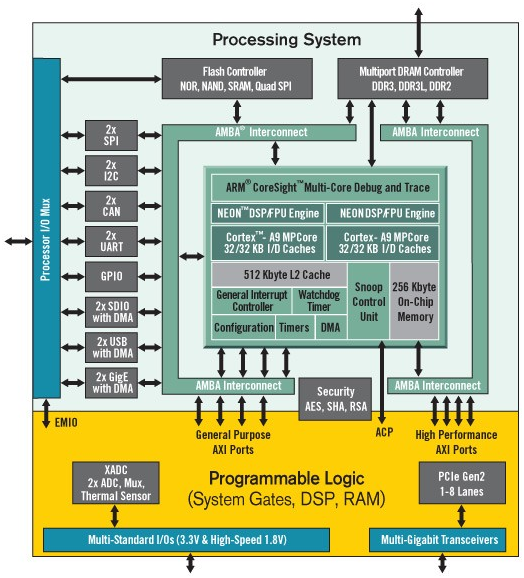
\includegraphics[width=\textwidth]{zynq.png}
	\caption{Architektura układu Zynq SoC \cite{zynq}.}
	\label{fig:zynq}
\end{figure}


\section{Moduł rejestrujący obraz}
\label{sec:pcam}

W~projekcie wykorzystano kolorową kamerę Digilent~PCAM~5C. 
Jest to~moduł przeznaczony do~użycia z~dedykowanymi płytkami rozwojowymi firmy Digilent. 
Jednym z~kompatybilnych układów jest ZYBO Z7-20. 
Podstawowe parametry modułu przedstawiono poniżej:
\begin{itemize}
	\item Rozdzielczość: 5 megapikseli,
	\item Matryca: OV5640,
	\item Interfejs danych: MIPI CSI-2,
	\item Złącze: 15-pinowe FFC.
\end{itemize}

%TODO2 Zdjęcie ? Ilustracja ? Może ew. obok tego Zybo, bo powinno się ładnie zmieścić.

Sposób podłączenia kamery i~układu ZYBO Z7-20 przedstawione zostały w~podrozdziale \ref{sec:integracja_uklad_kamera}.

\section{Platforma statku powietrznego}
\label{sec:platforma_statku_powietrznego}

W~projekcie wykorzystano dron sześciowirnikowy, znajdujący się na~wyposażeniu Studenckiego Koła Naukowego AVADER. 
Jego budowa była częścią innego projektu \cite{mgr}. 
Komponenty używanego bezzałogowago statku powietrznego to:
\begin{itemize}
	\item rama DJI F550,
	\item śmigła o średnicy równej 22,86~cm oraz skoku 12,7~cm,
	\item silniki DJI 2312/960KV z kontrolerami 420 LITE,
	\item czterokomorowa bateria LiPo o nominalnym napięciu 14,8~V i~pojemności 6450mAh, 
	\item nadajnik radiowy FrSky Taranis X9D Plus, odbiornik FrSky X8D,
	\item sterownik 3DR Pixhawk.
\end{itemize}

\section{Sterownik drona}
%TODO2 Fotos ?
\label{sec:autopilot}
Urządzeniem bezpośrednio komunikującym się z~kontrolerami silników jest sterownik. 
W~pracy wykorzystano urządzenie Pixhawk -- popularny kontroler lotu ogólnego przeznaczenia, który jest dostępny na~otwartej licencji. %TODO2 a nie raczej jego obprogramowanie
Jego główne parametry~to:
\begin{itemize}
	\item procesor Cortex-M4F z zegarem 168 MHz,
	\item czujniki: akcelerometr, żyroskop, kompas magnetyczny, barometr i~zewnętrzny moduł GPS,
	\item interfejsy: UART, CAN, I2C, SPI,
	\item wejście karty SD,
	\item zewnętrzny przełącznik bezpieczeństwa uzbrajania,
	\item wielokolorowa dioda pokazująca stan pracy.
\end{itemize}
Konfiguracja sterownika jest możliwa przy użyciu programu \textit{Mission Planner}. 
Jest to~aplikacja przeznaczona dla~stacji naziemnej umożliwiająca:
\begin{itemize}
	\item strojenie czujników autopilota,
	\item monitorowanie stanu sterownika (uzbrojenie silników, orientacja statku powietrznego),
	\item planowanie, zapisywanie i~wgrywanie planów autonomicznych misji statku powietrznego,
	\item pobieranie i~analizowanie dzienników misji.
\end{itemize} 

Po~instalacji oprogramowania ArduPilot sterownik umożliwia pracę w~różnych trybach. 
Dostępne są~23 tryby wbudowane, z~czego 5 jest rekomendowanych \cite{pixhawk_modes}. 
Istnieją tryby wspierające różne poziomy i~typy stabilizacji, a~zadania wykonywane przez autopilota w~każdym z~nich nieco się różnią. 
Poniżej przedstawiono podsumowanie najważniejszych cech rekomendowanych trybów:
\begin{itemize}
	\item \textit{Stablize} -- pozwala operatorowi na~manualne sterowanie dronem, stabilizując jego pochylenie i~przechylenie,
	\item \textit{Alt Hold} -- kontroluje ustawienie mocy silników w~celu utrzymania wysokości,
	\item \textit{Loiter} --  utrzymuje aktualną pozycję drona, jeśli operator nie wydaje żadnych poleceń,
	\item \textit{Return-To-Launch} --  dron unosi się na~domyślną wysokość 15~metrów, a~następnie powraca do~miejsca, w~którym został uzbrojony. Tryb ten wymaga sygnału GPS,
	\item \textit{Auto} --  dron realizuje zaprogramowaną wcześniej misję, poruszając się po~zdefiniowanych punktach. Wymagany jest sygnał GPS.
\end{itemize}

Z~punktu widzenia autonomicznego lądowania, odpowiednim trybem do~sterowania dronem jest tryb \textit{Guided}.
Umożliwia on~bowiem wysyłanie dronowi komend dotyczących zmiany szybkości i~lotu w~określonym kierunku. %TODO2 nieco niejasna konstrukcja może szybkości i kierunku lotu ?
Zazwyczaj wykorzystywana jest komunikacja ze~stacją naziemną drogą radiową (przy użyciu programu Mission Planner), lecz wysyłanie komend przez urządzenie umieszczone na~platformie drona również jest możliwe.
Komunikacja taka przebiega z~wykorzystaniem protokołu MAVLink (ang. \textit{Micro Air Vehicle Link}).
Umożliwia on~przesyłanie danych i~komend z~wykorzystaniem prawie każdego rodzaju transmisji szeregowej \cite{mavlink_basics}. 
W~tabeli \ref{tab:frame} przedstawiono opis ramki protokołu.
\begin{table}[]
	\caption{Opis ramki protokołu MAVLink}
	\label{tab:frame}
	\begin{tabular}{|l|l|l|l|}
		\hline
		Indeks bajtu & Zawartość                                                                         & Wartość        & Uwagi                                                                                                                            \\ \hline
		0            & Znak początku pakietu                                                             & 0xFE           & Wskazuje na początek nowego pakietu.                                                                                             \\ \hline
		1            & Długość danych                                                                    & n (0-255)      & Informuje o liczbie przesyłanych danych.                                                                                          \\ \hline
		2            & Sekwencja pakietu                                                                 & 0-255          & \begin{tabular}[c]{@{}l@{}}Wartość zwiększana przy każdej transmisji.\\ Umożliwia detekcję utraty pakietów.\end{tabular}         \\ \hline
		3            & ID systemu                                                                        & 1-255          & \begin{tabular}[c]{@{}l@{}}ID systemu wysyłającego. Umożliwia odróżnienie\\ różnych sieci.\end{tabular}                          \\ \hline
		4            & ID komponentu                                                                     & 0-255          & \begin{tabular}[c]{@{}l@{}}ID komponentu wysyłającego. Umożliwia \\ odróżnienie różnych komponentów w jednej sieci.\end{tabular} \\ \hline
		5            & ID wiadomości                                                                     & 0-255          & \begin{tabular}[c]{@{}l@{}}Oznacza typ wiadomości i umożliwia jej\\ zdekodowanie.\end{tabular}                                   \\ \hline
		6--n+6      & Dane                                                                              & (0-255) bajtów & Zawartość wiadomości. Zależy od jej ID.                                                                                          \\ \hline
		n+7--n+8    & \begin{tabular}[c]{@{}l@{}}Suma kontrolna\\ (młodszy i starszy bajt)\end{tabular} & \multicolumn{2}{l|}{Umożliwia wykrycie błędów transmisji}                                                                                         \\ \hline
	\end{tabular}
\end{table}

Kwestię połączenia autopilota i układu ZYBO~Z7-20 opisano w~podrozdziale \ref{sec:integracja_plytka_autopilot}.

\section{Laserowy czujnik wysokości}
\label{sec:laser}
W~projekcie do~pomiaru wysokości wykorzystano urządzenie Garmin Lidar Lite v3. 
Jego główne parametry~to:
\begin{itemize}
	\item Napięcie zasilania -- 5 V,
	\item Zasięg pomiaru -- 40 m,
	\item Dokładność -- 2,5 cm (pomiar do 5 m), 
	\item Wykorzystywana długość fali -- 905 nm,
	\item Interfejsy -- I2C, PWM z~zewnętrznym wyzwalaniem pomiaru.
\end{itemize}

%TODO2 Zdjęcie.

%TODO2 Proszę jeszcze opisać to radio (i zdjęcie) - nie zaszkodzi, że tam będzie. Nawet jeśli nie działa.

\chapter{Implementacja i ewaluacja modelu programowego}
\label{cha:implementacja_modelu}

\iffalse
W~rozdziale szczegóły związane z~implementacją systemu. 
Ważną rolę w~tworzeniu kolejnych modułów odegrał model programowy, czyli program napisany w~dowolnym języku programowania i~wykonywany na~komputerze~PC, którego działanie oddaje funkcjonalność modułu tworzonego w~sprzęcie.
Porównanie wyników działania modelu programowego i~symulacji modułu daje informację o~poprawności implementacji. 
Model programowy, wraz z~uzasadnieniem użycia poszczególnych modułów, przedstawiono na~początku rozdziału.
Następnie opisano wszystkie wykonane komponenty, od~przesłania obrazu przez kamerę, do~wysyłania komend do~autopilota.
\fi
%TODO2 Modyfikacja opisu(wykonane)
Ważną rolę w~tworzeniu kolejnych modułów odegrał model programowy, czyli program napisany w~dowolnym języku programowania i~wykonywany na~komputerze~PC, którego działanie oddaje funkcjonalność modułu tworzonego w~sprzęcie.
Porównanie wyników działania modelu programowego i~symulacji modułu daje informację o~poprawności implementacji. 
Model programowy, wraz z~uzasadnieniem użycia poszczególnych operacji, przedstawiono na~początku rozdziału.
Następnie skupiono się na~wyborze kształtu i~koloru znacznika umieszczonego na~lądowisku.
Na~koniec przedstawiono opis badań związanych z~kątem widzenia kamery przy~różnych ustawieniach rozdzielczości.

\section{Opis zastosowanych operacji przetwarzania wizyjnego}
\label{sec:opis_operacji}
Model programowy został napisany w pakiecie Matlab przy wykorzystaniu funkcji dostępnych w~bibliotece \textit{Image Processing Toolbox}. 
Pozwoliło to~na~szybkie prototypownie systemu wizyjnego, składającego się~z:
\begin{itemize}
	\item konwersji z~przestrzeni RGB do YCbCr,
	\item binaryzacji ze~stałymi progami,
	\item mediany,
	\item otwarcia,
	\item indeksacji jednoprzebiegowej wyznaczającej pole powierzchni i~prostokąt otaczający obiektów.
\end{itemize}

Piksel w~przestrzeni barw YCbCr opisują trzy składowe: Y (luminancja), Cb (chrominancja, która wyraża różnicę między luminancją, a~kolorem niebieskim) oraz Cr (chrominancja, która wyraża różnicę między luminancją,~a~kolorem czerwonym). 
Zaletą stosowania tej przestrzeni barw jest oddzielenie sygnału luminancji od~sygnałów chrominancji, co pozwala na realizację przetwarzania sygnału przy mniejszej zależności od~oświetlenia.
Zastosowanie binaryzacji pozwala na~oddzielenie znacznika od~tła. 
Na~wyjściu modułu znajdują się tylko dwa rodzaje pikseli: należące i~nienależące do~obiektu (rys. \ref{fig:bin_1}).

Na~obrazie często znajdują się jednak inne niewielkie obszary (zakłócenia), które zostały błędnie wykryte. Pozostawienie ich na~wejściu modułu indeksacji zwiększyłoby niepotrzebnie liczbę nadawanych etykiet, która w~rozwiązaniach sprzętowych jest zwykle ograniczona (podrozdział \ref{subsec:indeksacja}).
Częściowym rozwiązaniem problemu jest zastosowanie mediany. 
Jest to~operacja kontekstowa, w~której pikselowi wyjściowemu przypisuje się wartość środkową uporządkowanego zbioru wartości pikseli z~otoczenia piksela wejściowego. 
Wykorzystanie mediany powoduje znaczne zmniejszenie błędnych obszarów, jednakże niekiedy na~obrazie obecne są~nadal małe grupy białych pikseli nienależących do~obiektu (rys. \ref{fig:median_1}).

Z~tego powodu zdecydowano się na~wykorzystanie operacji morfologicznych. 
Erozja i~dylatacja to~operacje, w~których pikselowi wyjściowemu przypisuje się wartość odpowiednio najmniejszego i~największego piksela w~sąsiedztwie piksela wejściowego. 
Sąsiedztwo piksela określa kształt i~rozmiar elementu strukturalnego.  
Zastosowanie morfologicznego otwarcia, składającego się z~erozji i~dylatacji, pozwala niekiedy na~całkowite wyeliminowanie błędnych białych pikseli (rys. \ref{fig:opened_1}).
W~projekcie założono jednak, że błędne piksele mogą nie zostać całkowicie usunięte i~powzięto próbę poradzenia sobie z~tym problemem.
Indeksacja jednoprzebiegowa to~operacja pozwalająca na wyodrębnienie z~obrazu cech poszczególnych obiektów. Obiekty rozumiane są~jako grupy połączonych ze~sobą pikseli. 
Ze~względu na~wykorzystywany w~dalszej analizie współczynnik kształtu, obliczano prostokąt otaczający i~pole obiektów. 
%TODO2 Dalej nie ma informacji dlaczego to jest potrzebne. W sensie, że zakłada Pan obecnośc więcej niż jednego obiektu !(wykonane)

\begin{figure}
	\centering
	\begin{subfigure}{0.4\textwidth}
		\centering
		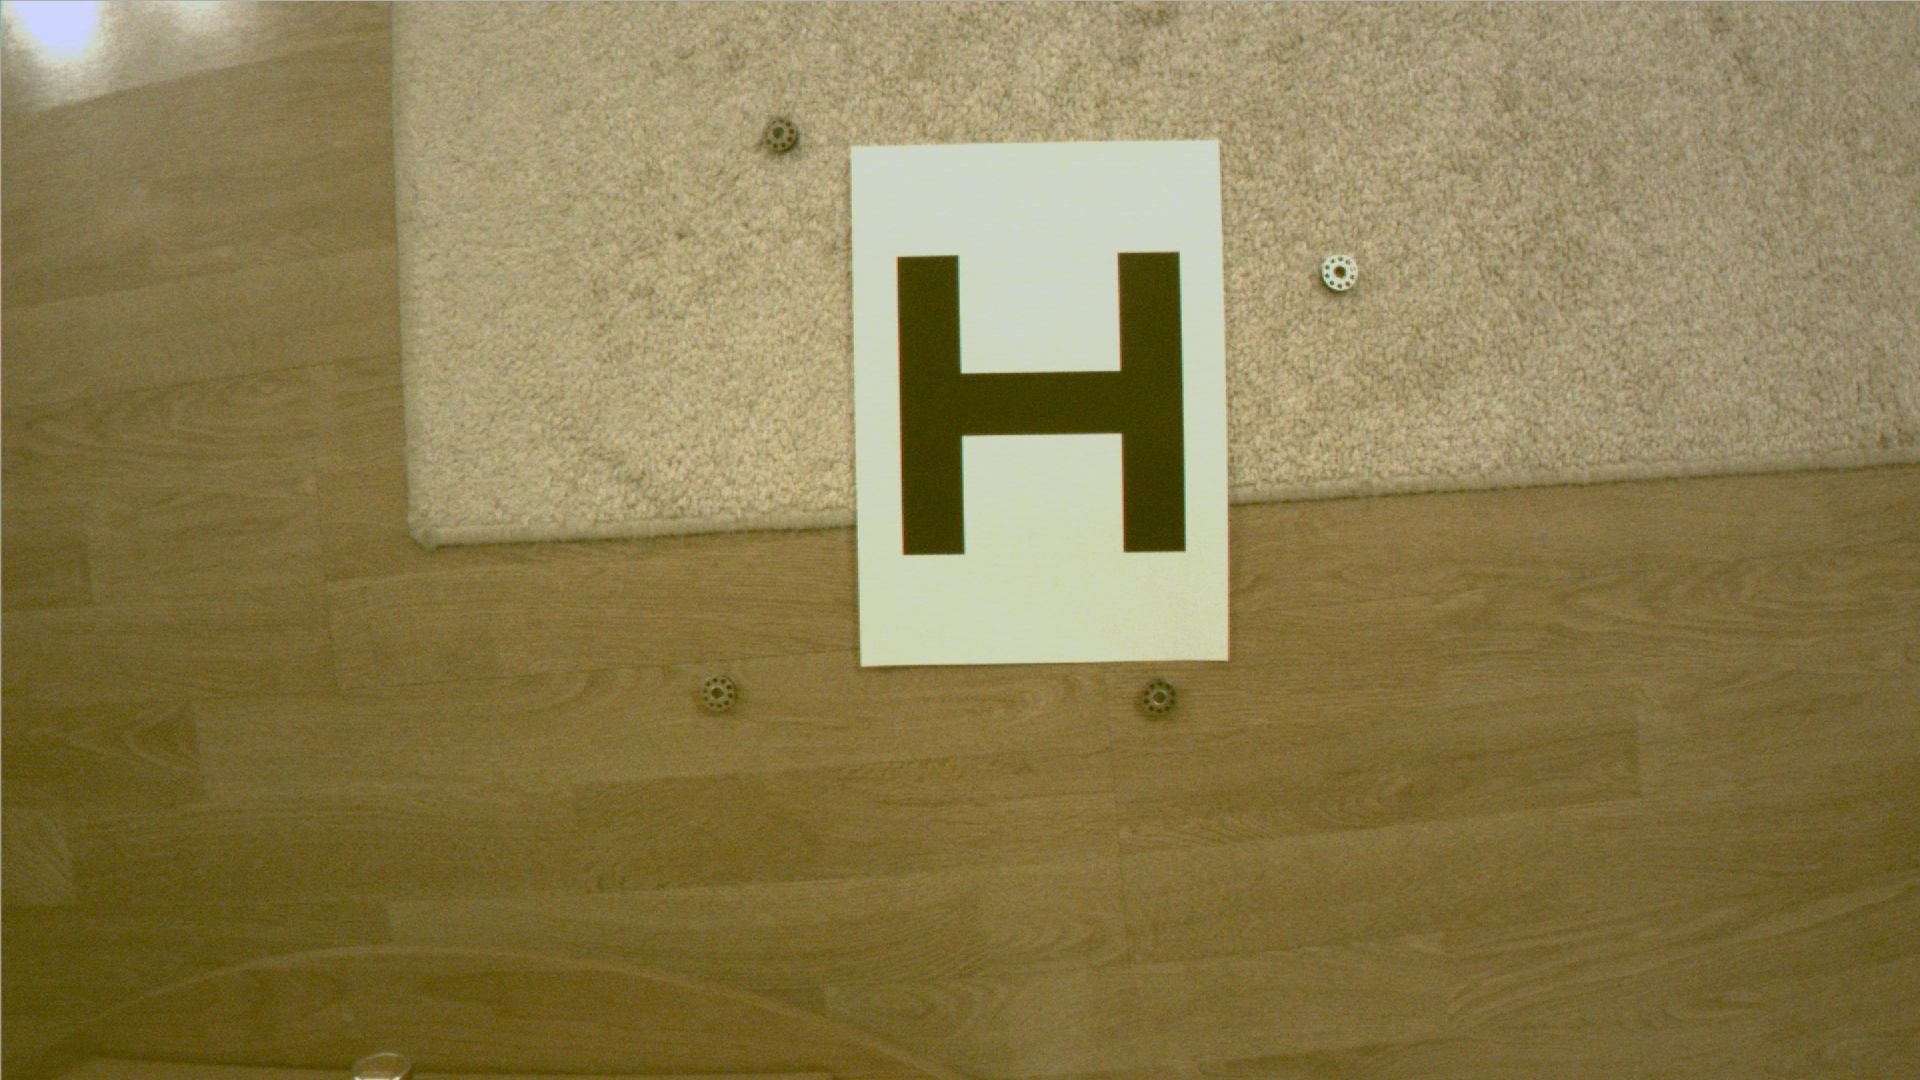
\includegraphics[width=\textwidth]{h.jpg}
		\caption{Obraz wejściowy.}
		\label{fig:h}
	\end{subfigure}
	\begin{subfigure}{0.4\textwidth}
		\centering
		
\includegraphics[width=\textwidth]{bin.jpg}
		\caption{Rezultat binaryzacji.}
		\label{fig:bin_1}
	\end{subfigure}\\
	\begin{subfigure}{0.4\textwidth}
		\centering
		
\includegraphics[width=\textwidth]{median.jpg}
		\caption{Obraz po medianie}
		\label{fig:median_1}
	\end{subfigure}
	\begin{subfigure}{0.4\textwidth}
		\centering
		
\includegraphics[width=\textwidth]{opened.jpg}
		\caption{Wynik otwarcia}
		\label{fig:opened_1}
	\end{subfigure}
	\caption{Przykładowe rezultaty binaryzacji, mediany i~otwarcia obrazu.}
	\label{fig:operacje}
\end{figure}

%TODO2 Przydałby się obraz wejściowy. I nie ma potrzeby dawać tego takiego dużego. 4 obrazy w układzie 2x2 wystarczą.(wykonane)


\section{Wybór znacznika} 
\label{sec:wybor_znacznika}

Autonomiczne lądowanie drona w~oparciu o~system wizyjny wymaga wyposażenia lądowiska w~marker. 
Jego wygląd musi umożliwiać łatwą detekcję miejsca lądowania. 
Z~powodu wykonywania operacji na~zewnątrz, znacznik powinien również ułatwiać znalezienie go~w~zmiennych warunkach (zachmurzenie, cień).

\subsection{Kształt}
\label{subsec:ksztalt} 
Detekcja kształtów może być realizowana na~różne sposoby. 
Najprostszym jest progowanie współczynników kształtu, do~bardziej zaawansowanych należy wyspecjalizowana deskrypcja cech (SIFT (ang. \textit{Scale-Invariant Feature Transform}), SURF (ang. \textit{Speeded-Up Robust Features}), HOG (ang. \textit{Histogram of Oriented Gradients})) i~użycie klasyfikatorów (kNN (ang. \textit{k Nearest Neighbours}), SVM (ang. \textit{Support Vector Machine}), sieci neuronowe). %TODO2 skróty trzeba rozwinąć(wykonane)
W~implementowanej pierwszej wersji systemu zdecydowano się na~klasyfikację przy użyciu współczynnika kształtu.

Cechami obiektu łatwymi do~wyliczenia w~systemie potokowym są~pole figury i~najmniejszy prostokąt, w~którym figura się mieści (prostokąt otaczający). 
Postanowiono zatem wykorzystać współczynnik kształtu przedstawiony we~wzorze \ref{eq:wspolczynnik}.\\
\begin{equation} \label{eq:wspolczynnik}
W=\frac{P_p}{P_o}
\end{equation}
Gdzie:
\begin{eqwhere}[2cm]
	\item[$W$] współczynnik kształtu,
	\item[$P_p$] pole prostokąta otaczającego,
	\item[$P_o$] pole obiektu.
\end{eqwhere}
Aby~taki współczynnik umożliwiał detekcję należało dobrać odpowiedni kształt znacznika. 
Zdecydowano się na~krzyż, gdyż przy każdej jego orientacji pole prostokąta jest znacznie większe od~pola obiektu. Dodatkowo, zastosowanie krzyża wydłużonego może dostarczyć informacji o~orientacji znacznika.
%TODO2 Nic nigdzie nie pisze Pan o orientacji. Wiem, że nie ma detekcji, ale jakieś zdanie komentarza ?(wykonane)
\subsection{Kolor}
\label{subsec:kolor}

Kolor znacznika powinien umożliwiać jego łatwą segmentację. 
Z~tego powodu pożądane jest silne skontrastowanie figury i~tła. 
Najbardziej naturalnym rozwiązaniem jest rozważenie kontrastu w~przestrzeni barw RGB, gdyż taki sygnał jest dostarczany przez kamerę.

\begin{figure}[h]
	\centering
	\begin{subfigure}{0.4\textwidth}
		\centering
		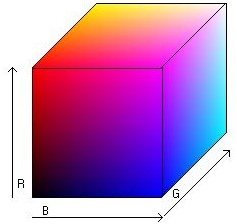
\includegraphics[width=0.5\textwidth]{szescian_rgb.jpg}
		\caption{Przedstawienie przestrzeni barw RGB w~postaci sześcianu \cite{obrazek_rgb}}
		\label{fig:szescian_rgb}
	\end{subfigure}%
	\begin{subfigure}{0.4\textwidth}
		\centering
		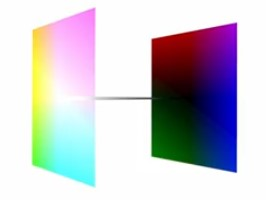
\includegraphics[width=0.5\textwidth]{szescian_ycbcr.jpg}
		\caption{Przekroje sześcianu przestrzeni YCbCr \cite{obrazek_ycbcr}}
		\label{fig:szescian_ycbcr}
	\end{subfigure}%
	\caption{Modele przestrzeni RGB i YCbCr}
	\label{fig:modele_przestrzeni}
\end{figure}

W~przestrzeni RGB każdy piksel opisywany jest przez trzy składowe: czerwoną, zieloną i~niebieską. 
Możliwe jest przedstawienie tego systemu w~formie sześcianu (rys. \ref{fig:szescian_rgb}). 
Można wyznaczyć przekątną łączącą punkty, dla których wszystkie współrzędne są~identyczne. 
Rozciąga się ona od~koloru czarnego w~początku układu współrzędnych, do~białego dla~maksymalnych wartości składowych, przechodząc przez różne stopnie szarości. 
Wykorzystanie dużej odległości między kolorami i~użycie czarno-białego znacznika wydaje się zatem najprostszym pomysłem.

W~pierwszym kroku do testów przygotowano czarny znacznik na~białym tle. 
Kamerą PCAM 5C wykonano trzy zdjęcia przy różnym poziomie oświetlenia (Rys. \ref{fig:osw1}, \ref{fig:osw2}, \ref{fig:osw3}). Wykonanie takich zdjęć było możliwe po implementacji akwizycji ramek na~kartę~SD \ref{sec:image_sd}. %TODO2 tu odnośnik do dalszej części pracy(wykonane)
Po~przejściu na~obraz w~skali szarości, posługując się narzędziem \textit{roipoly} w~programie Matlab, obliczono histogramy obszaru znacznika (rys. \ref{fig:bw_hist1}, \ref{fig:bw_hist2}, \ref{fig:bw_hist3}).\\
\begin{figure}
	\centering
	\begin{subfigure}{0.4\textwidth}
		\centering
		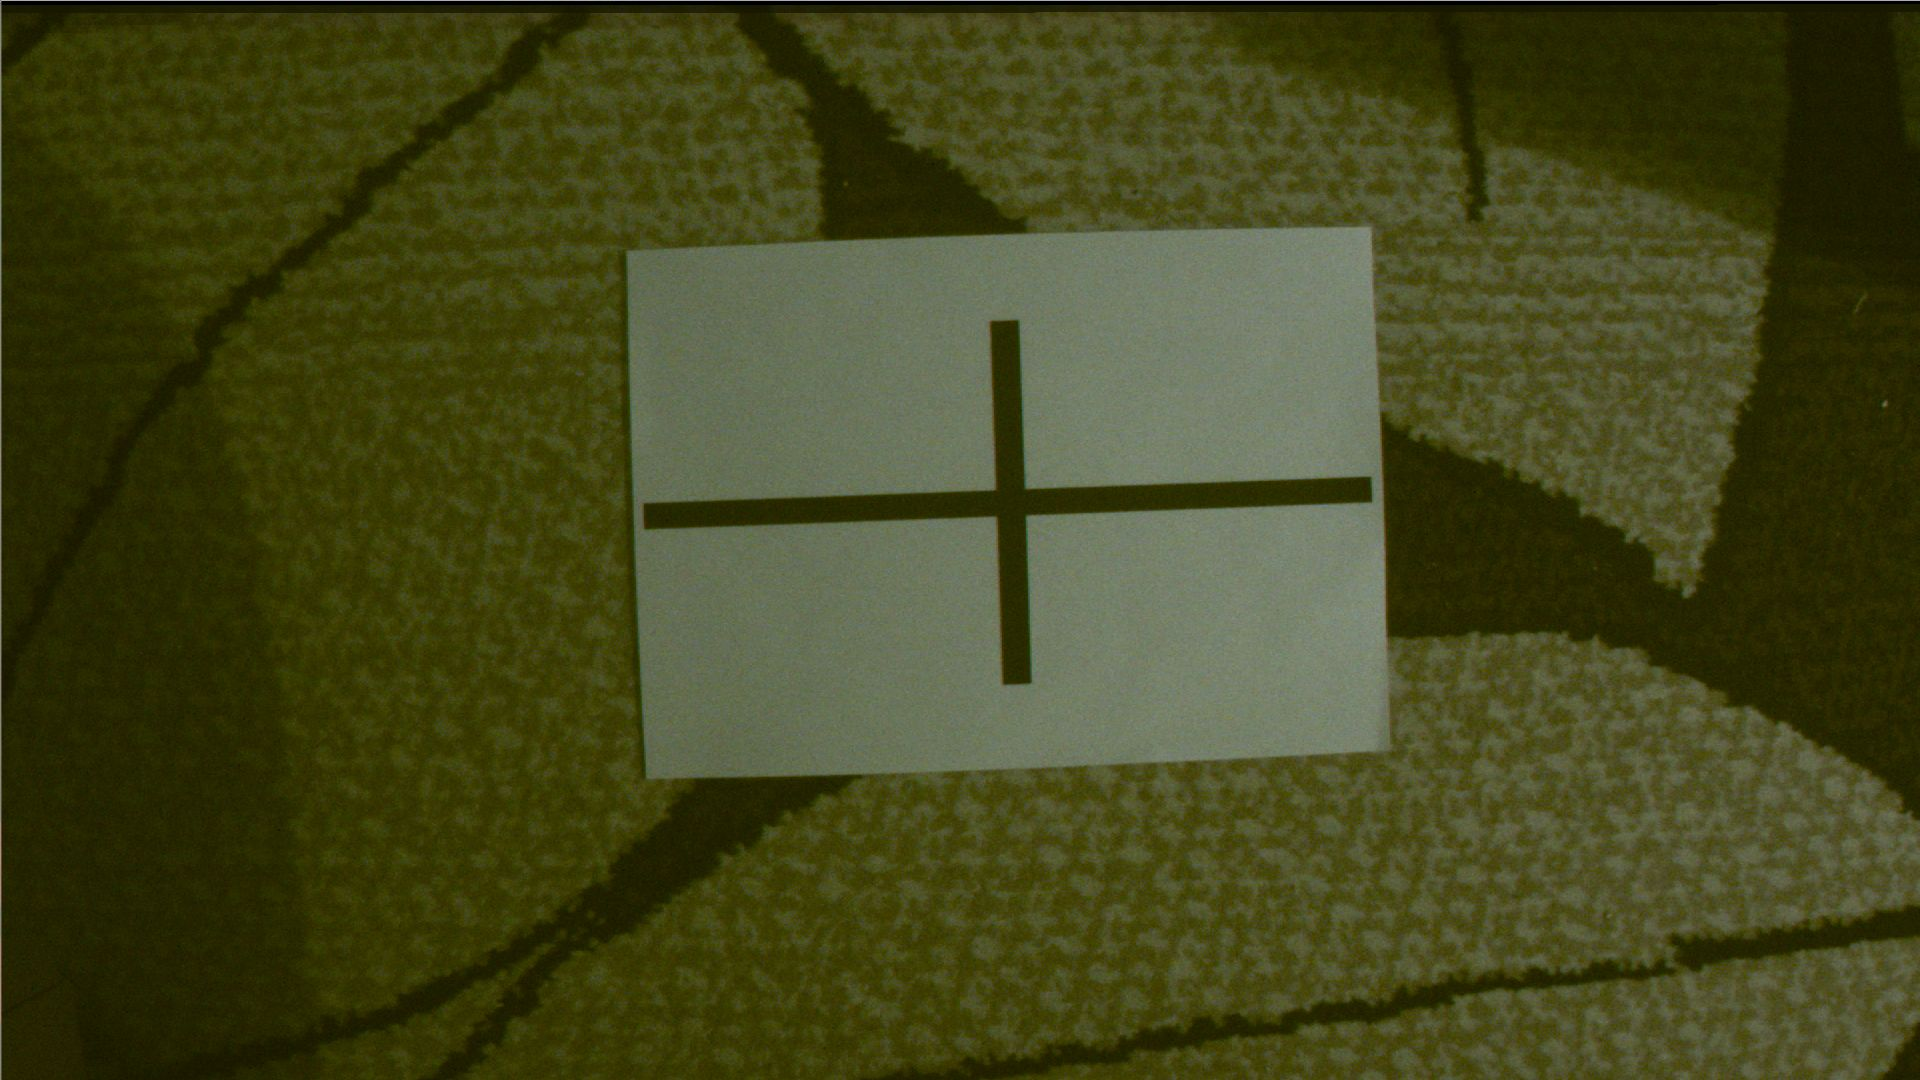
\includegraphics[width=0.98\textwidth]{rgb_ciemny.jpg}
		\caption{}
		\label{fig:osw1}
	\end{subfigure}%
	\begin{subfigure}{0.55\textwidth}
		\centering
		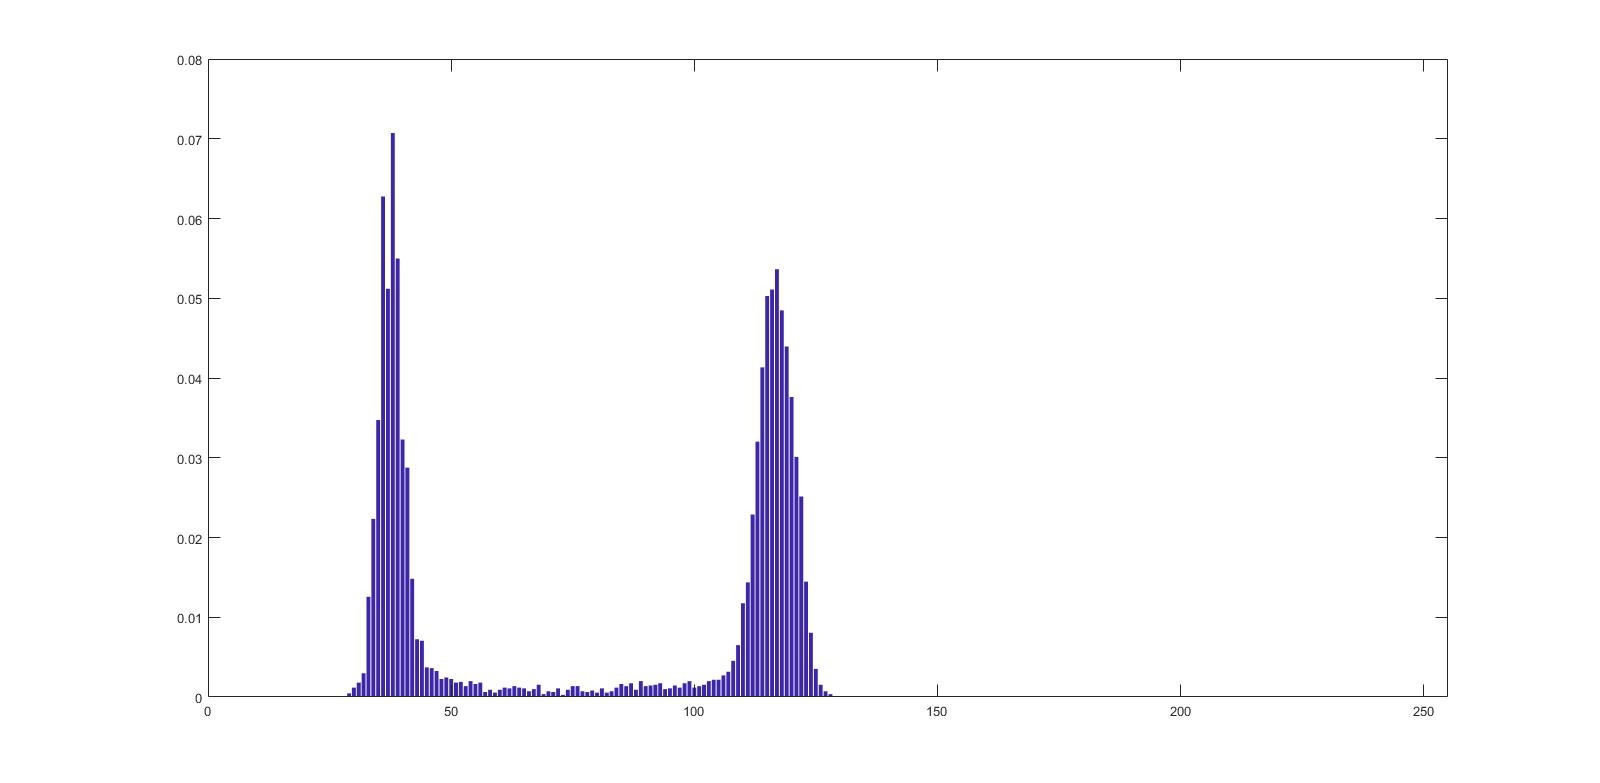
\includegraphics[width=0.98\textwidth]{bw_hist1.jpg}
		\caption{}
		\label{fig:bw_hist1}
	\end{subfigure}\\
	\begin{subfigure}{0.4\textwidth}
		\centering
		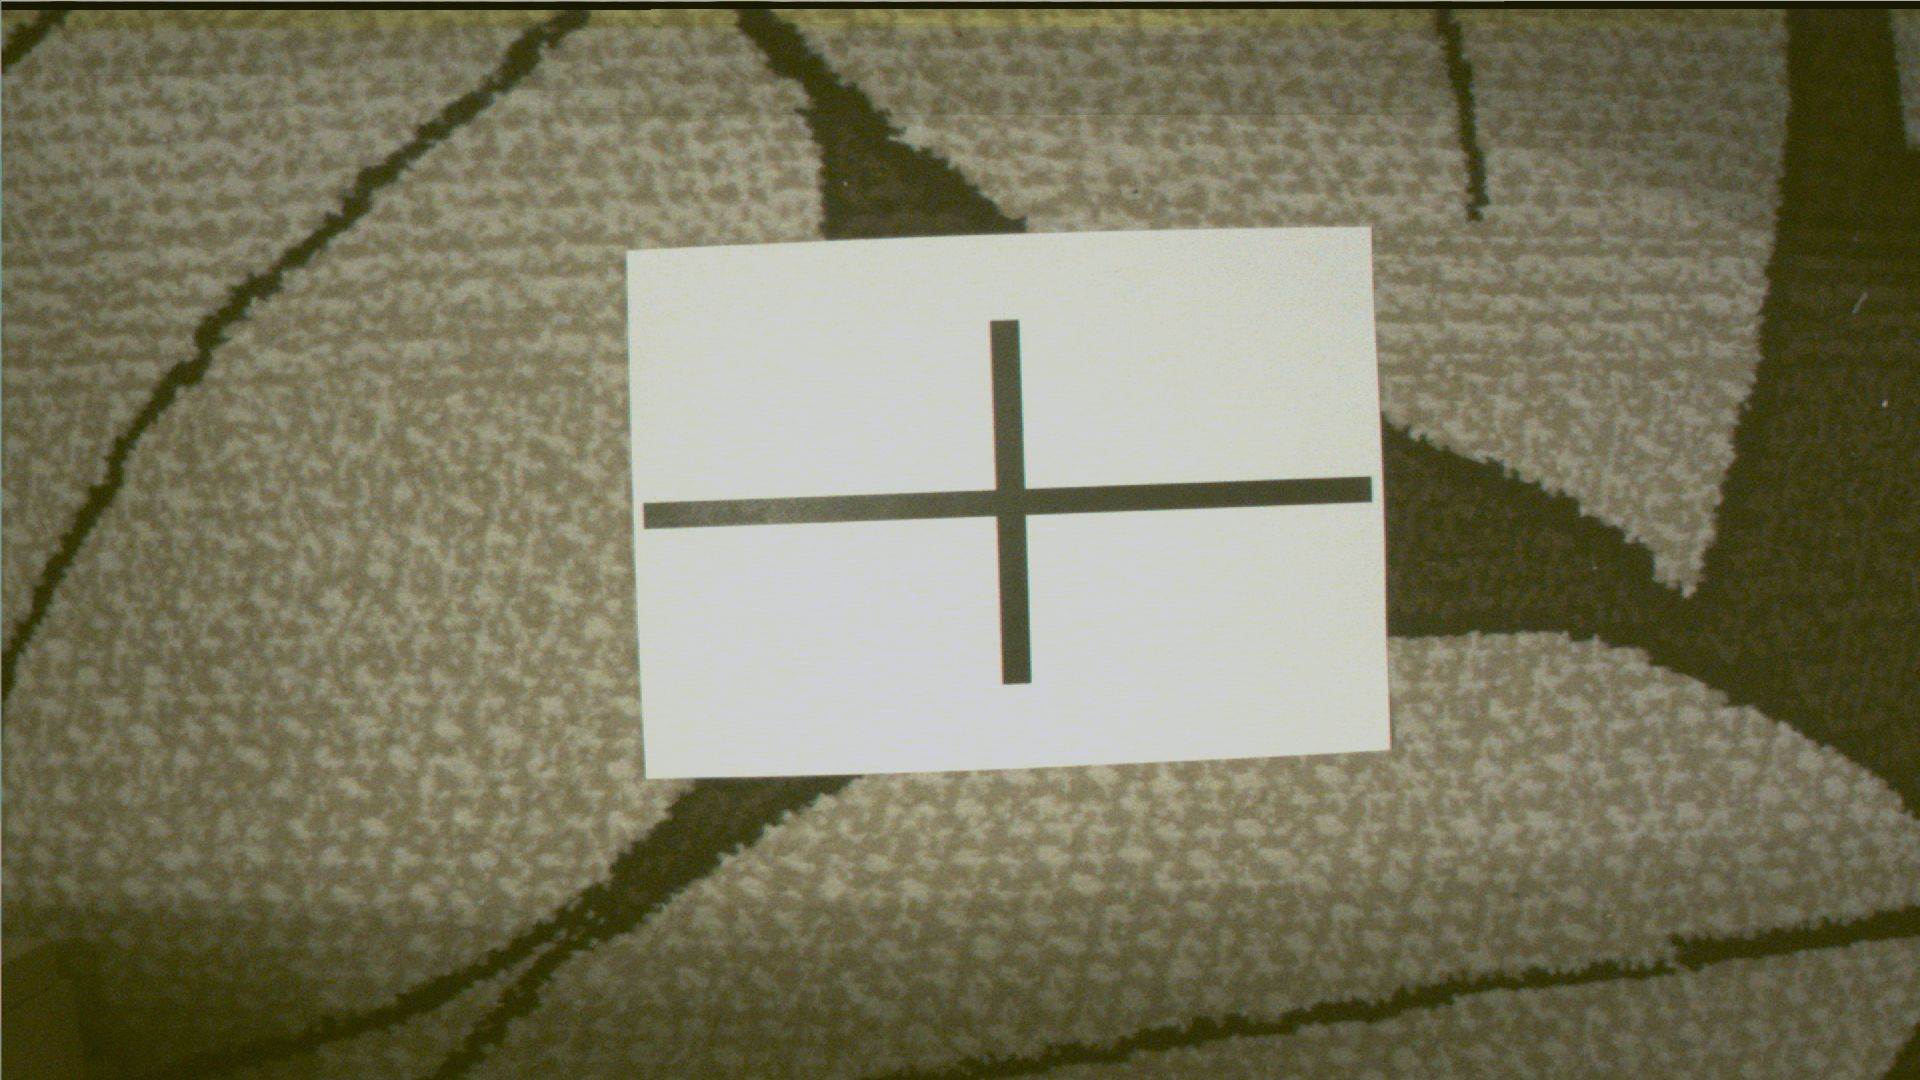
\includegraphics[width=0.98\textwidth]{rgb_sredni.jpg}
		\caption{}
		\label{fig:osw2}
	\end{subfigure}
	\begin{subfigure}{0.55\textwidth}
		\centering
		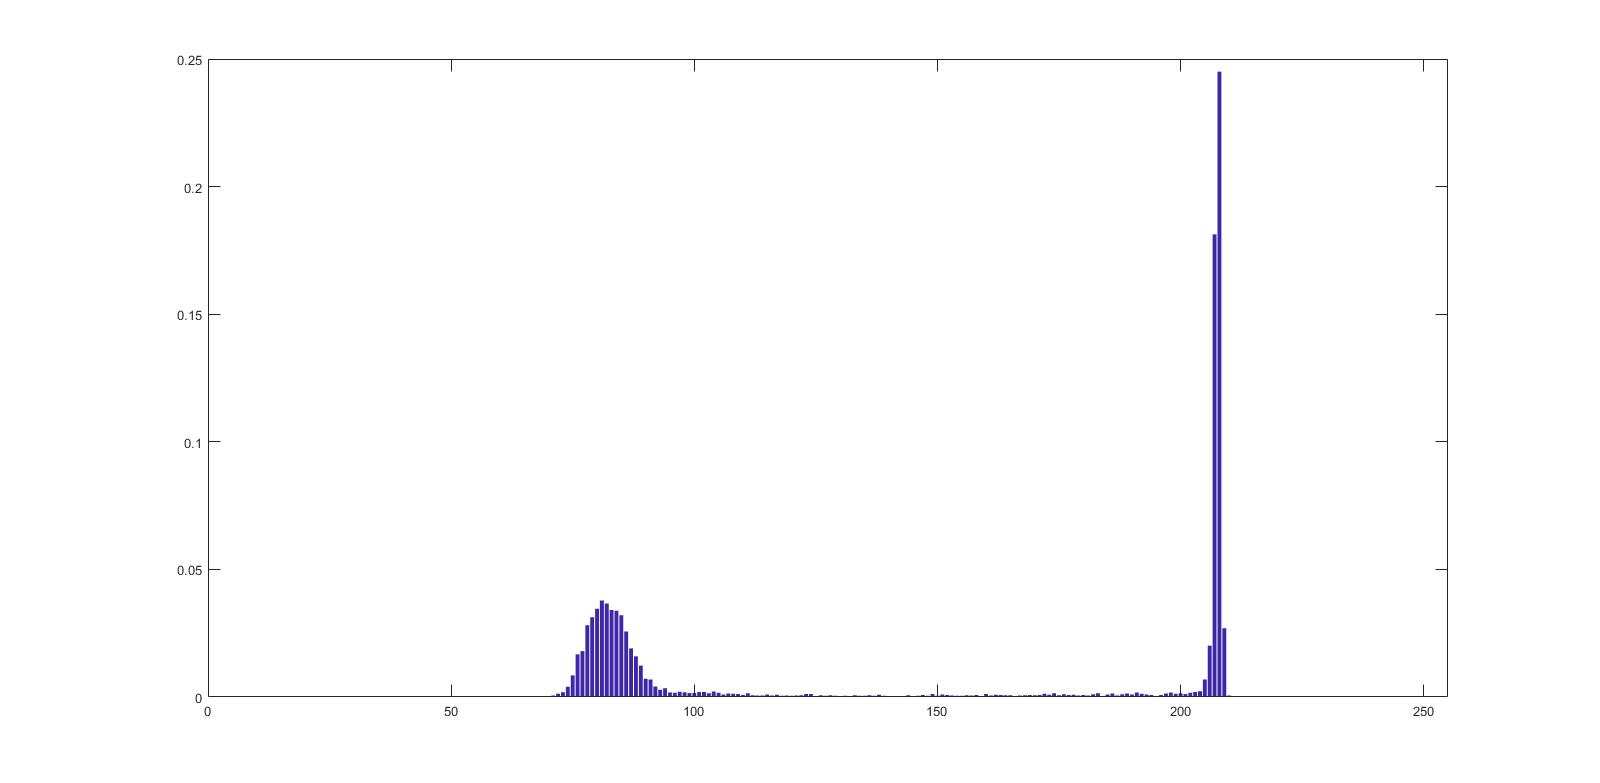
\includegraphics[width=0.98\textwidth]{bw_hist2.jpg}
		\caption{}
		\label{fig:bw_hist2}
	\end{subfigure}\\
	\begin{subfigure}{0.4\textwidth}
		\centering
		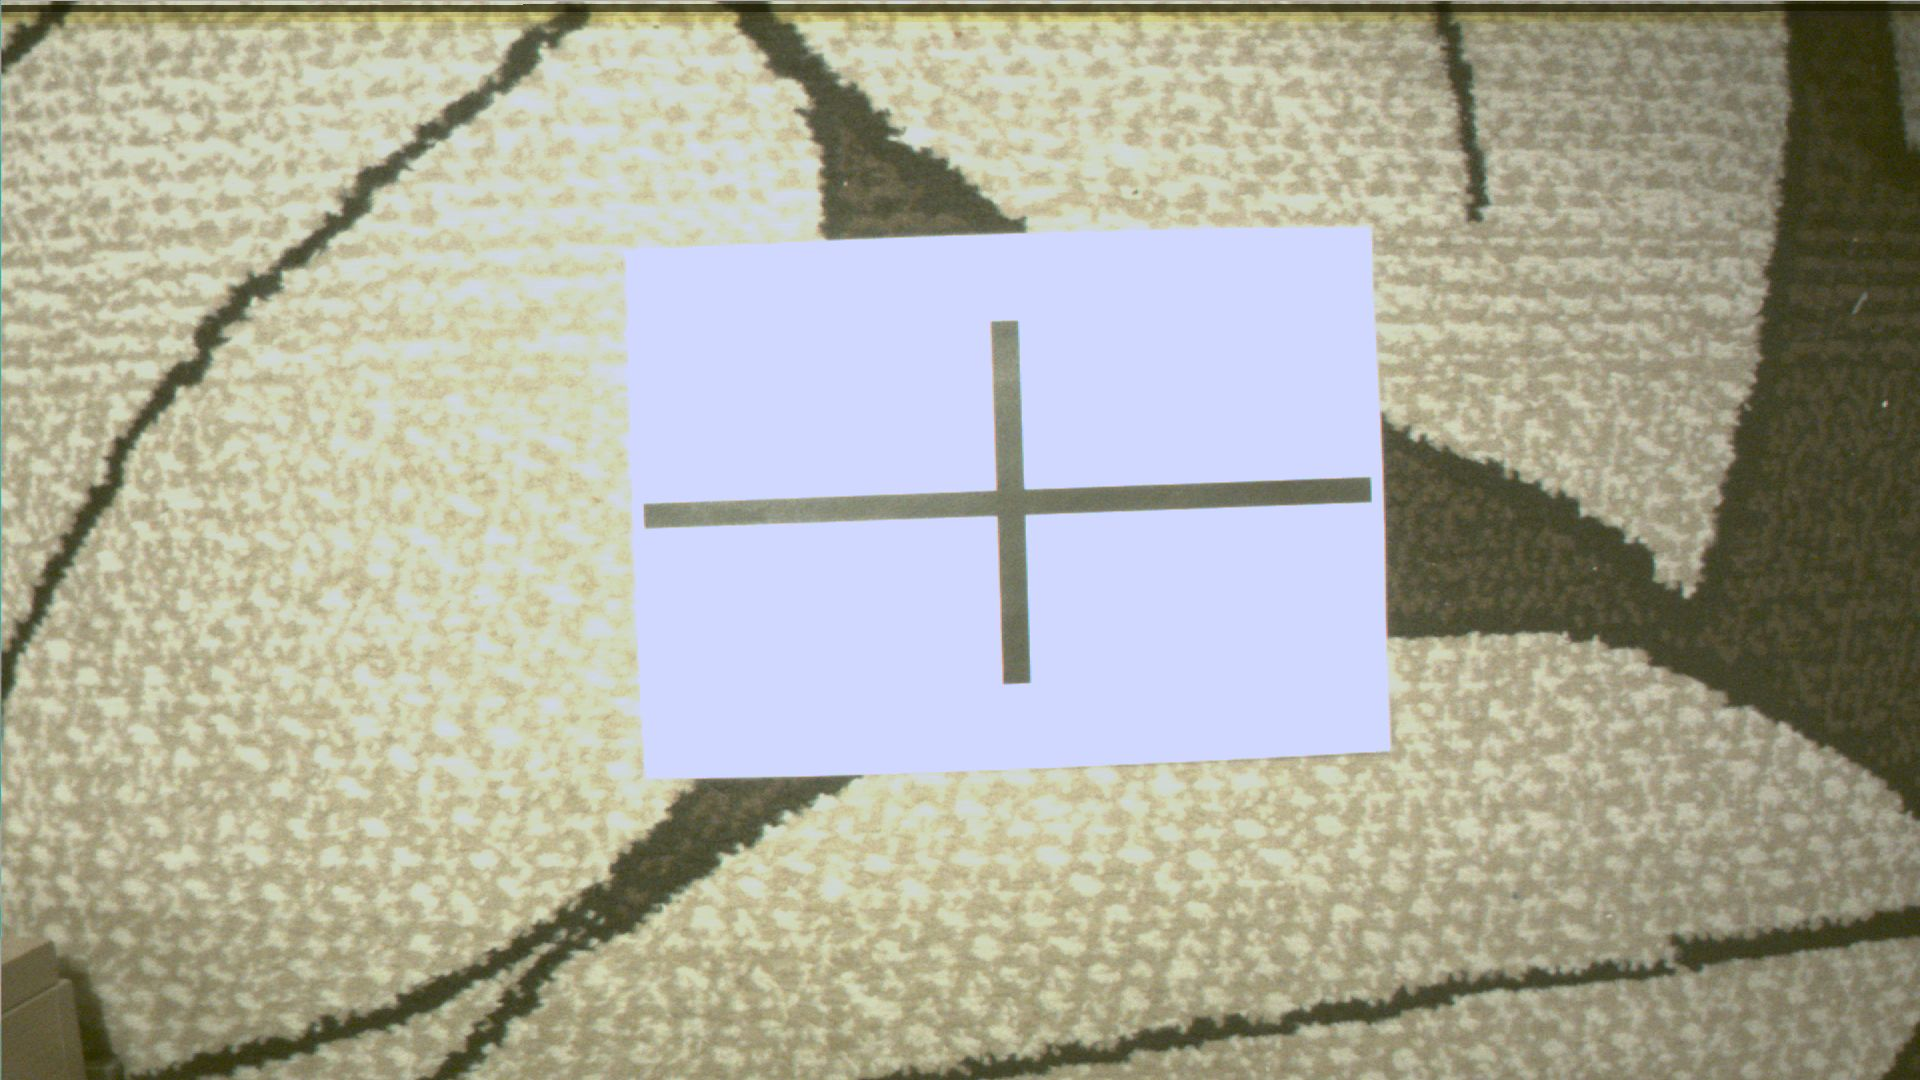
\includegraphics[width=0.98\textwidth]{rgb_jasny.jpg}
		\caption{}
		\label{fig:osw3}
	\end{subfigure}
	\begin{subfigure}{0.55\textwidth}
		\centering
		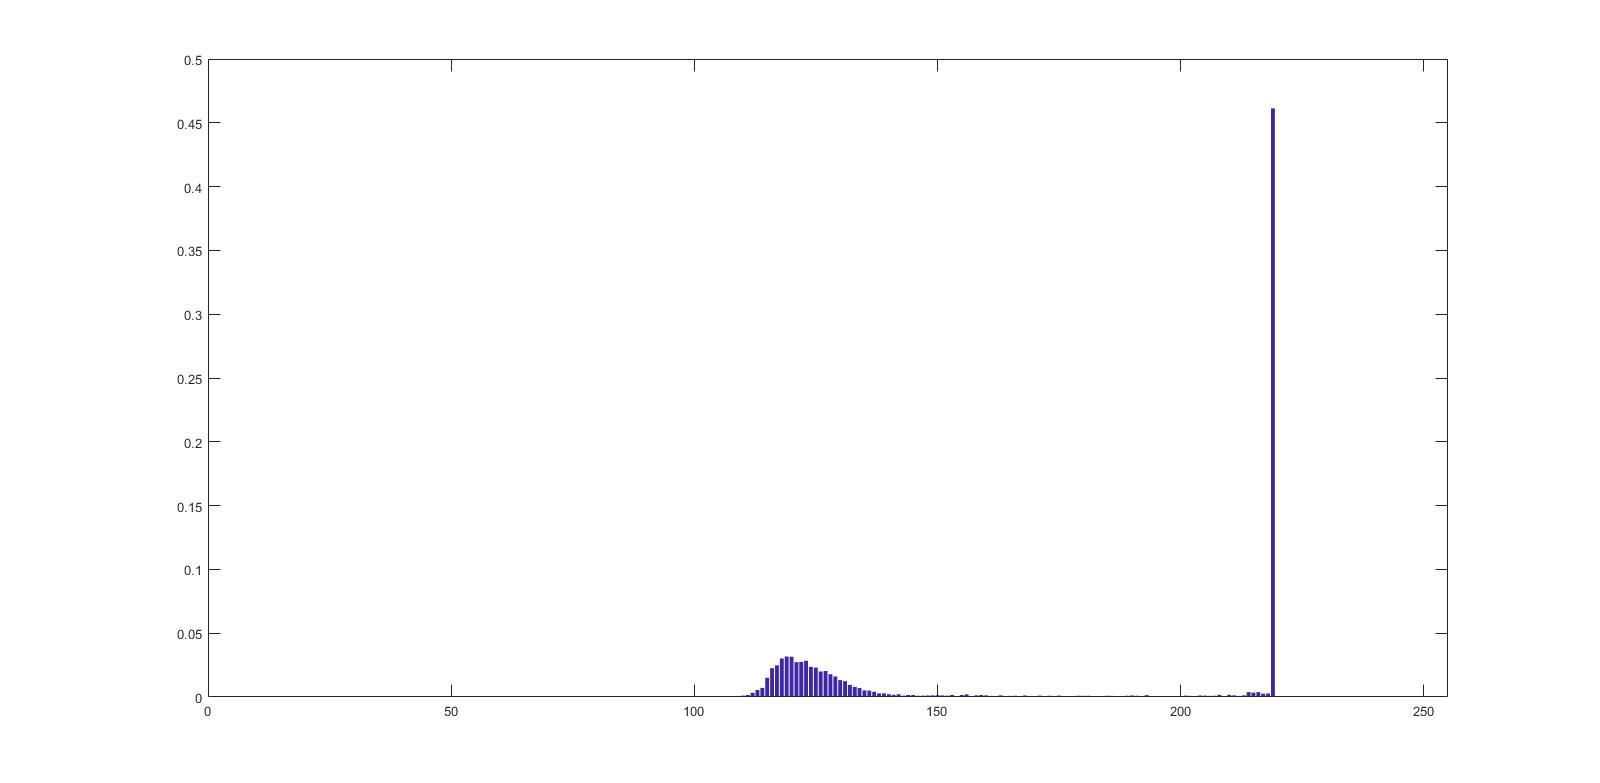
\includegraphics[width=0.98\textwidth]{bw_hist3.jpg}
		\caption{}
		\label{fig:bw_hist3}
	\end{subfigure}
	\caption{Zdjęcia pierwszej wersji znacznika wraz z~histogramami obszaru znacznika}
	\label{fig:zdjecia_wejsciowe}
\end{figure}

Analiza histogramów wskazuje na~silne uzależnienie położenia maksimów odpowiadających tłu i~znacznikowi od~oświetlenia.  %TODO2 raczej położenia maksimów odpowiadających tłu i znacznikowi.(wykonane)
Dla kolejnych obrazów, wartości progów binaryzacji mogłyby zawierać się w~zakresach: 50-100, 100-200, 150-210. Poziom białego tła dla obrazka najsłabiej oświetlonego jest mniejszy niż wartość czarnego koloru znacznika najlepiej oświetlonego. 
W~takiej sytuacji niemożliwy jest dobór stałego progu umożliwiającego skuteczną binaryzację.

Z~tego powodu zdecydowano się na~powtórzenie eksperymentu w~przestrzeni YCbCr. 
Tak jak opisano w~rozdziale \ref{sec:opis_operacji}, piksel w~tej przestrzeni opisuje współrzędna luminancji i~dwie składowe chrominacji. 
Podobnie jak w~przypadku RGB, przestrzeń YCbCr również da~się przedstawić w~postaci sześcianu. 
Tym razem skala szarości przebiega przez środek płaszczyzn Cb-Cr i~za zmianę poziomu szarości odpowiada współrzędna luminancji (rys. \ref{fig:szescian_ycbcr}). 
Dla~każdej wartości piksela informacja o~jasności oddzielona jest od~barwy.

Kolor znacznika określono jako czerwony, natomiast tło niebieskie, gdyż te~barwy znajdują się na~przeciwnych stronach płaszczyzny Cr-Cb. 
Zdjęcia wykonano przy takich samych poziomach oświetlenia jak poprzednio. 
Histogramy kolejnych obrazów przedstawiono na~rysunku \ref{fig:ycbcr_hist1}, \ref{fig:ycbcr_hist2}, \ref{fig:ycbcr_hist3}. 
\begin{figure}
	\centering
	\begin{subfigure}{0.45\textwidth}
		\centering
		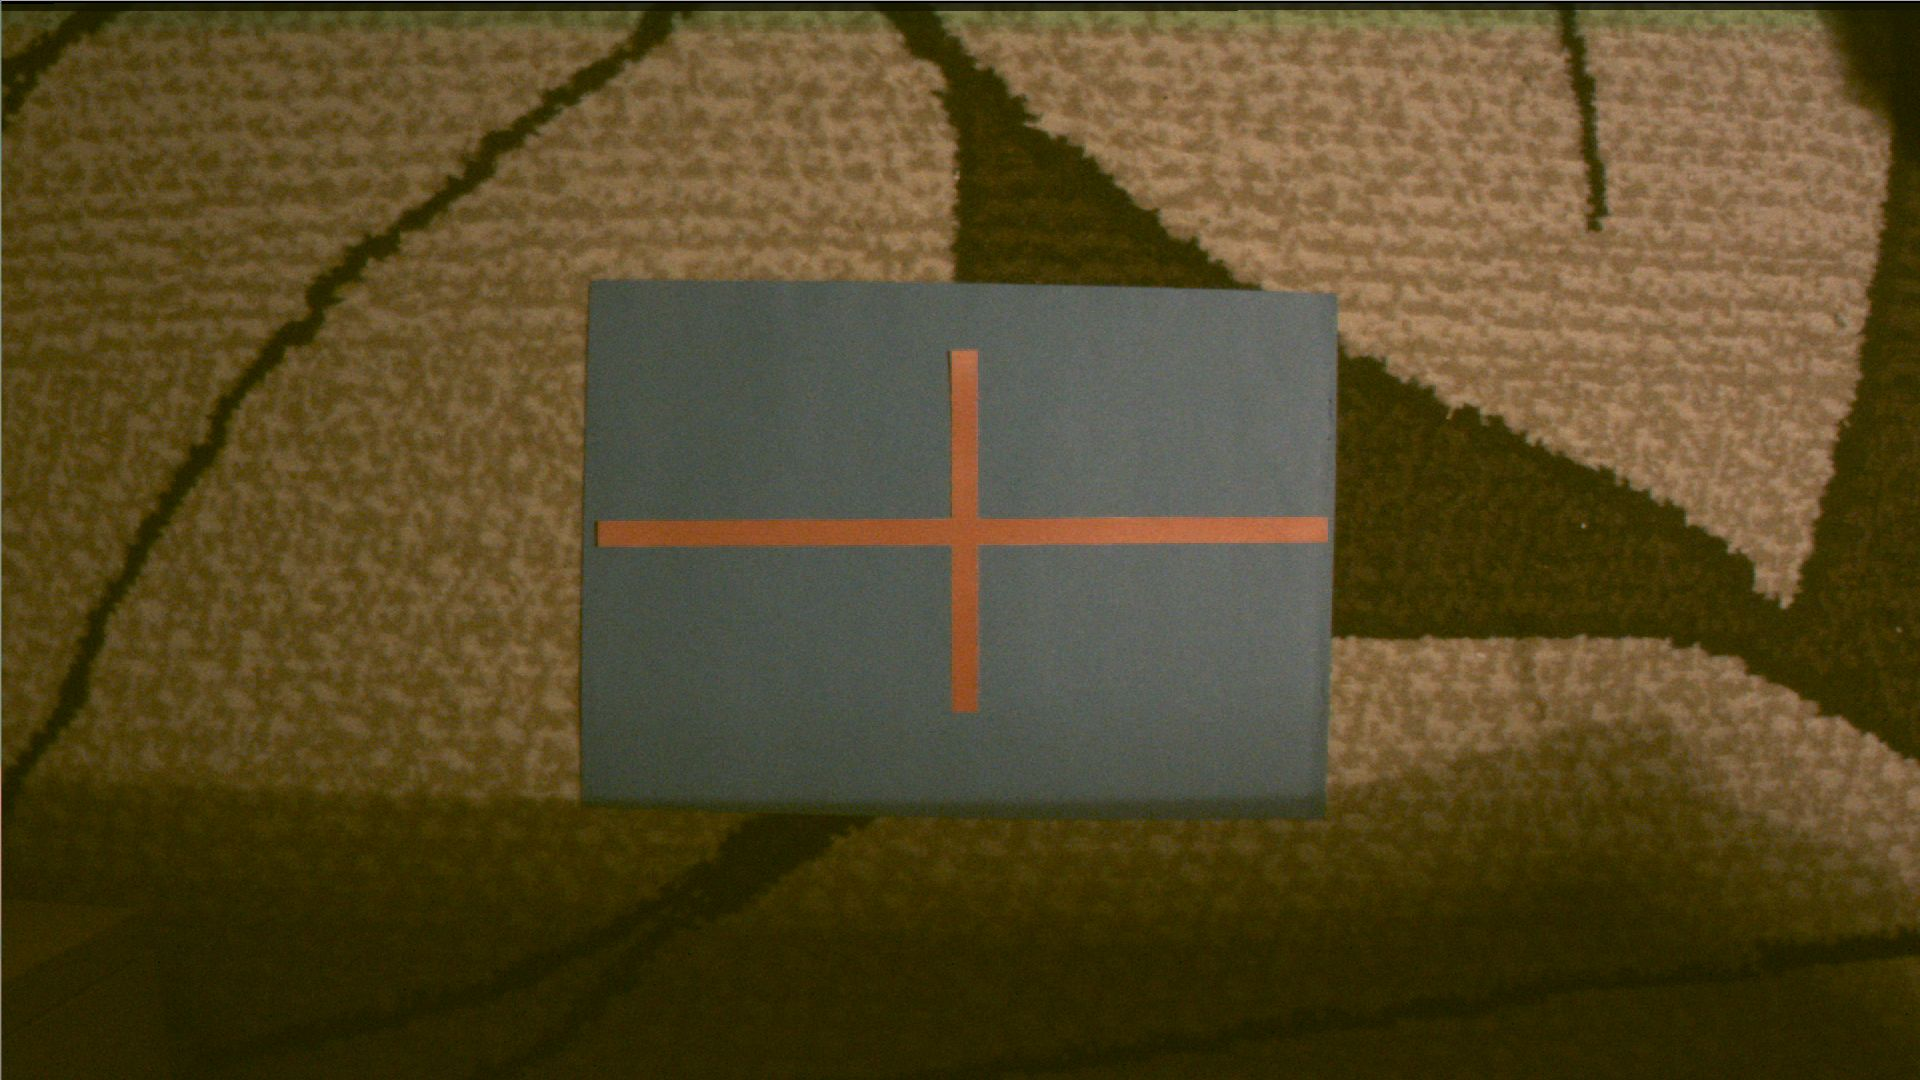
\includegraphics[width=0.9\textwidth]{ycbcr_ciemny.jpg}
		\caption{}
		\label{fig:ycbcr_1}
	\end{subfigure}
	\begin{subfigure}{0.45\textwidth}
		\centering
		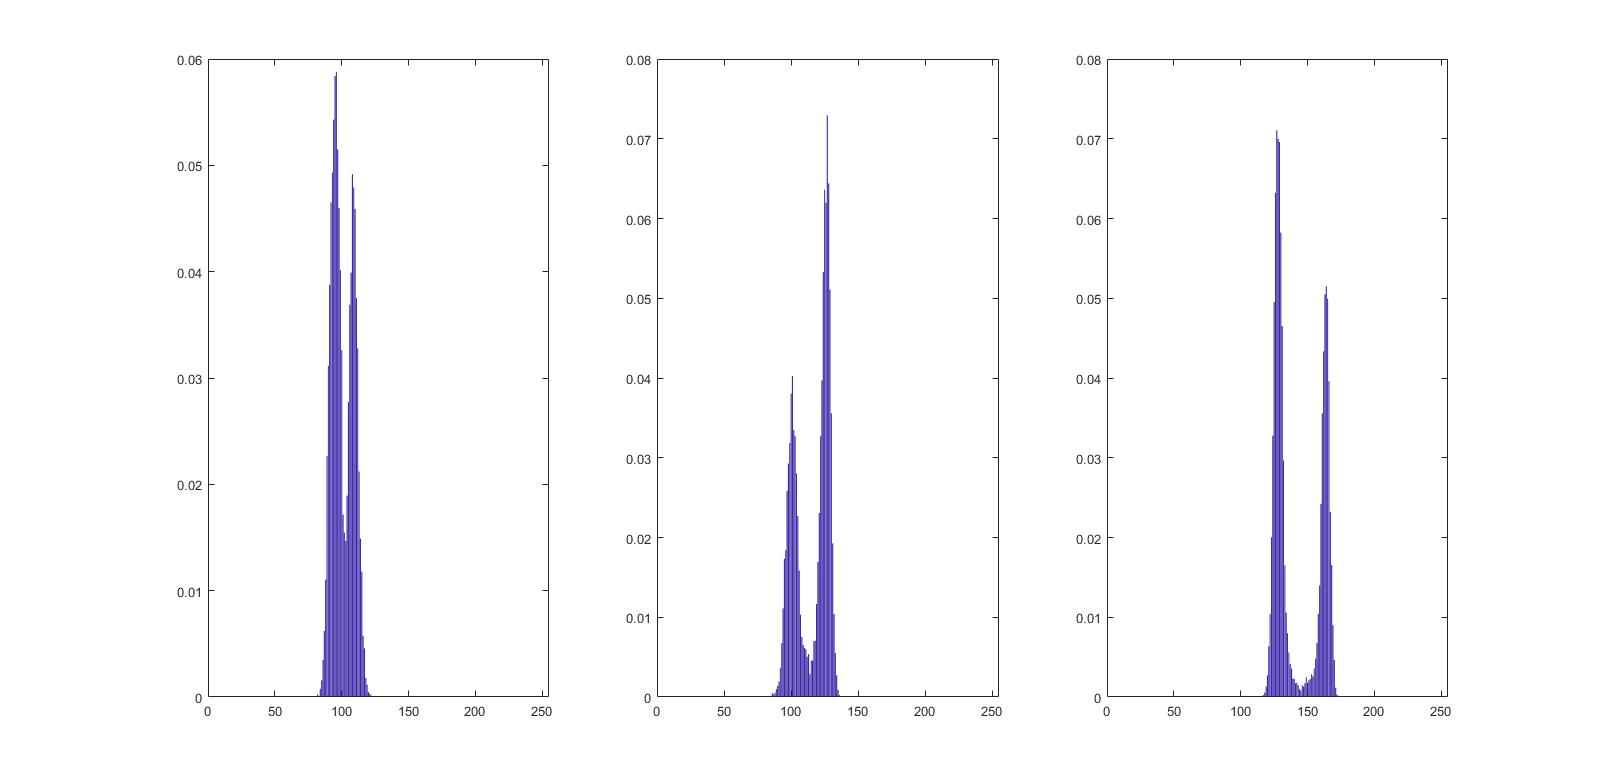
\includegraphics[width=0.9\textwidth]{ycbcr_hist1.jpg}
		\caption{}
		\label{fig:ycbcr_hist1}
	\end{subfigure}\\
	\begin{subfigure}{0.45\textwidth}
		\centering
		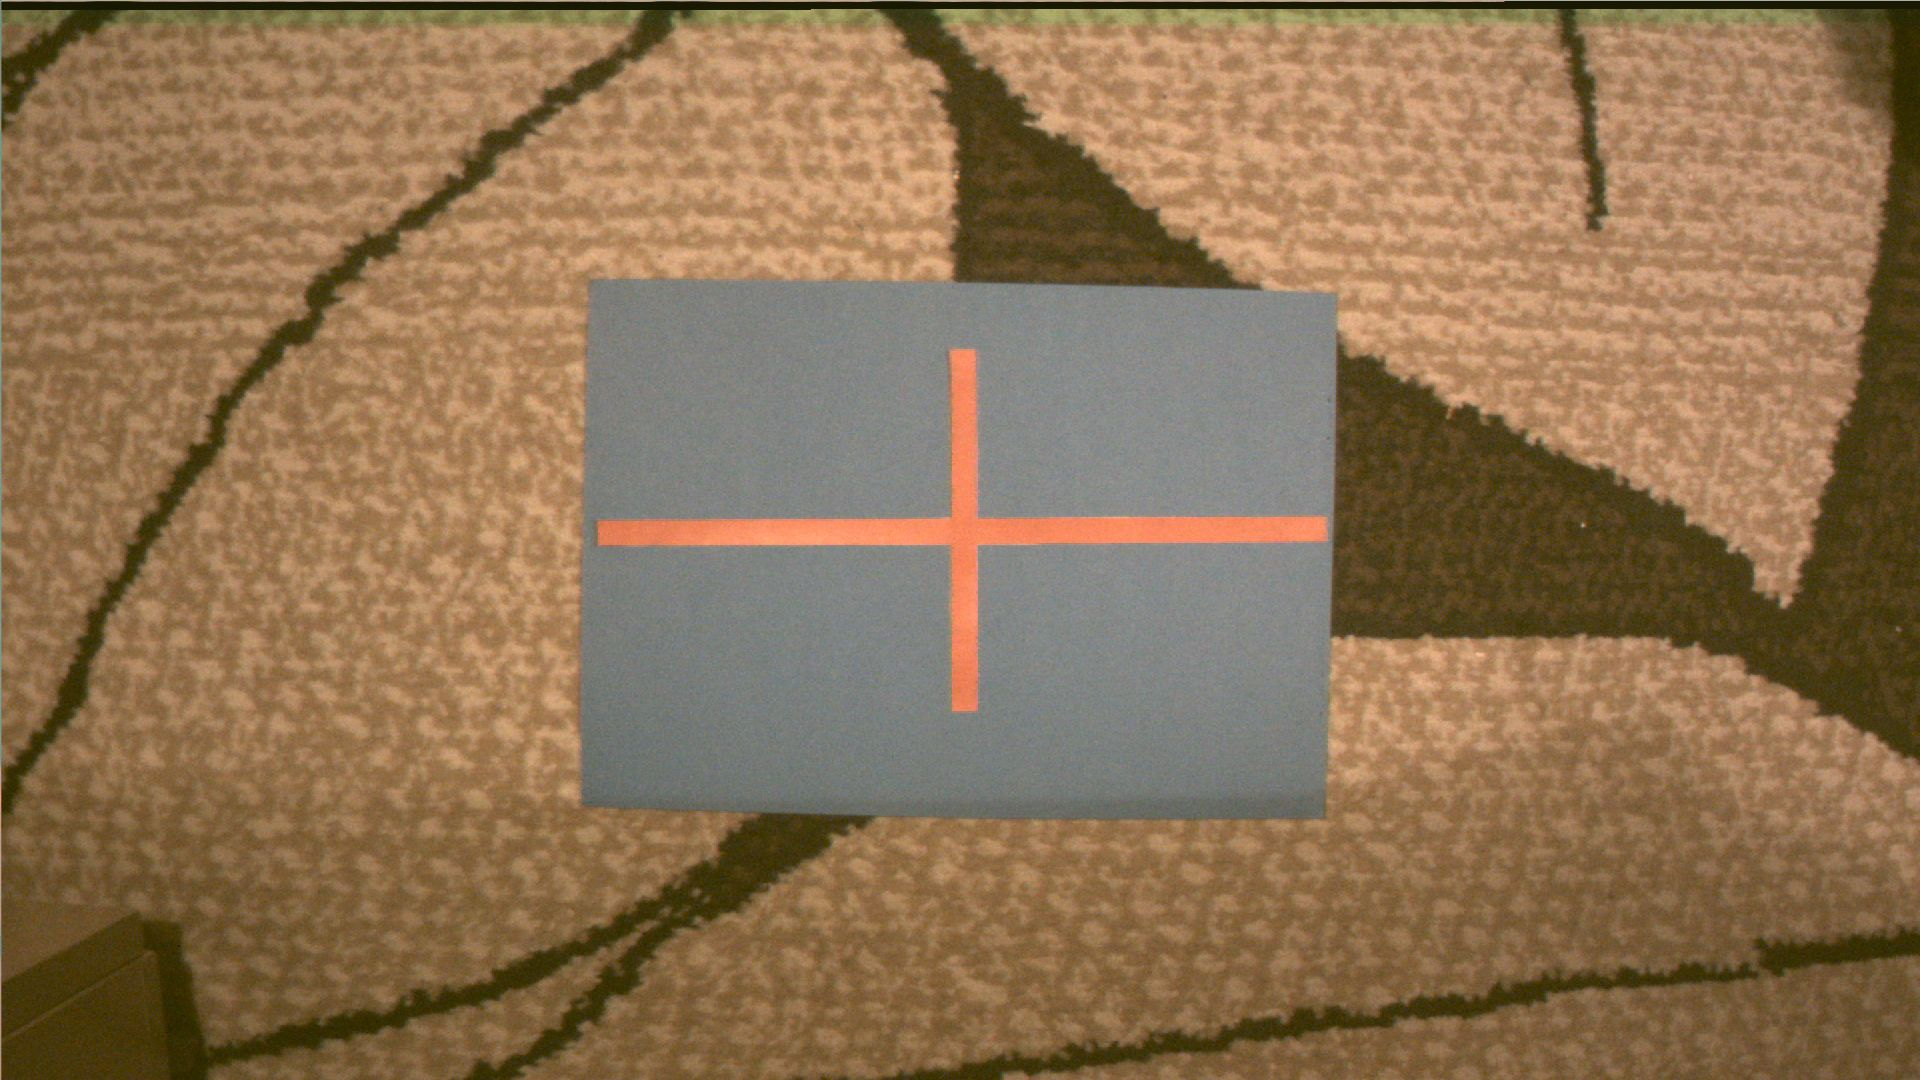
\includegraphics[width=0.9\textwidth]{ycbcr_sredni.jpg}
		\caption{}
		\label{fig:ycbcr_2}
	\end{subfigure}
	\begin{subfigure}{0.45\textwidth}
		\centering
		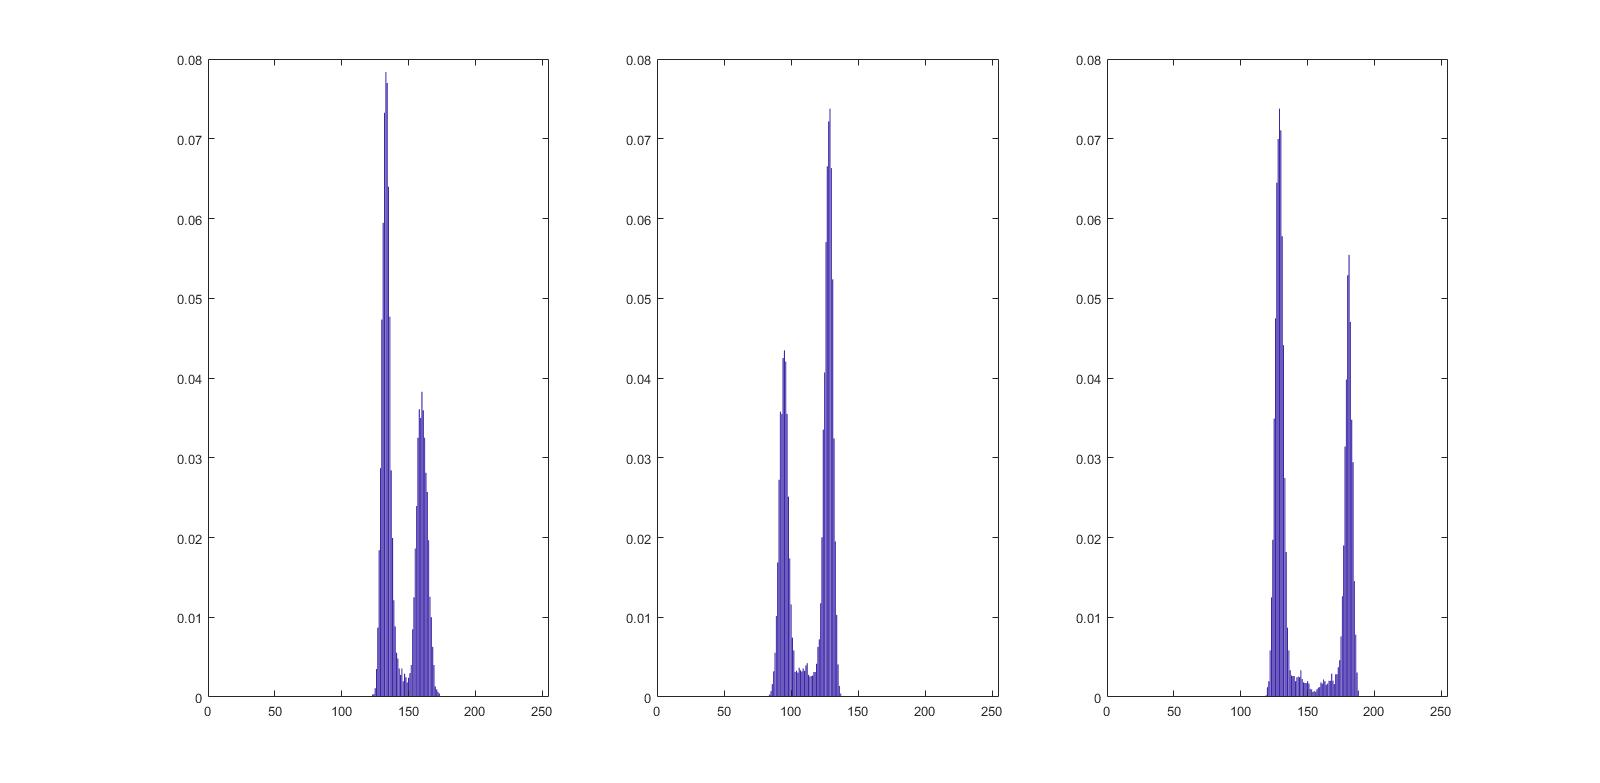
\includegraphics[width=0.9\textwidth]{ycbcr_hist2.jpg}
		\caption{}
		\label{fig:ycbcr_hist2}
	\end{subfigure}\\
	\begin{subfigure}{0.45\textwidth}
		\centering
		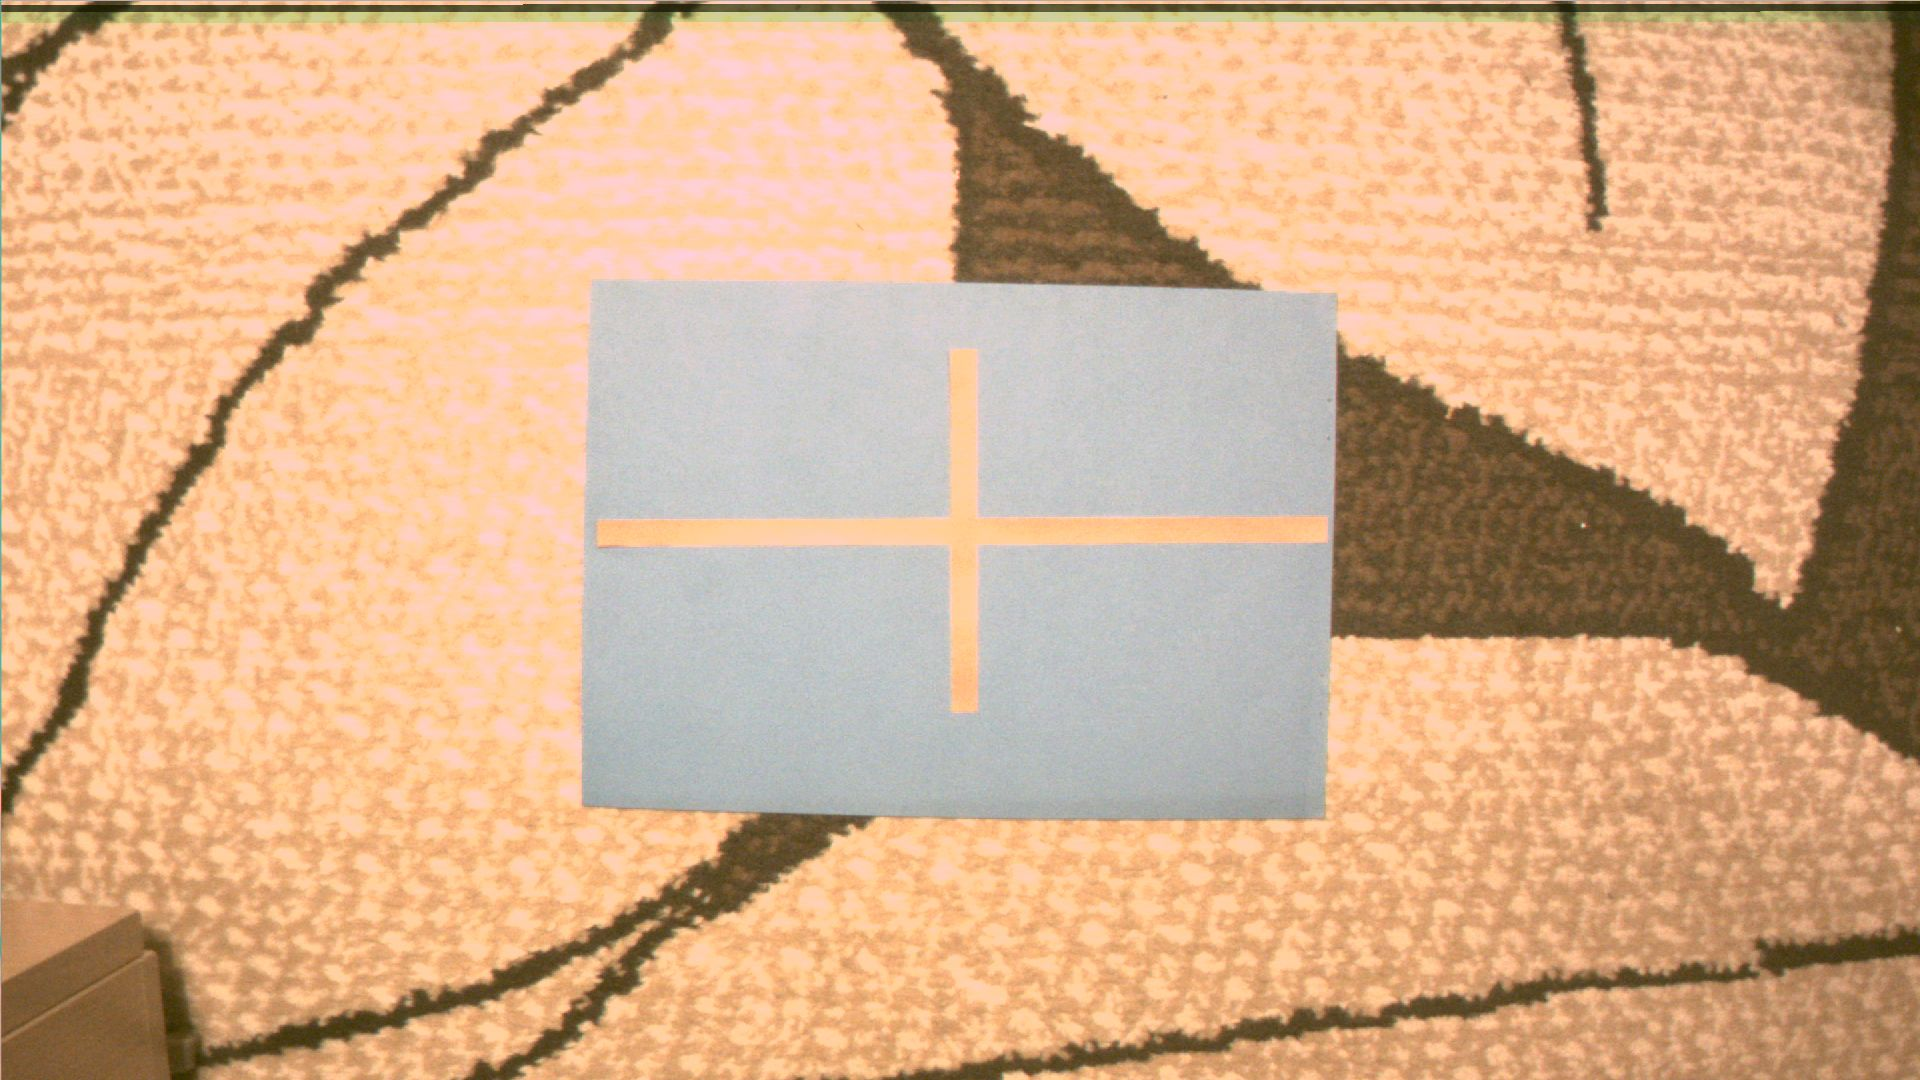
\includegraphics[width=0.9\textwidth]{ycbcr_jasny.jpg}
		\caption{}
		\label{fig:ycbcr_3}
	\end{subfigure}
	\begin{subfigure}{0.45\textwidth}
		\centering
		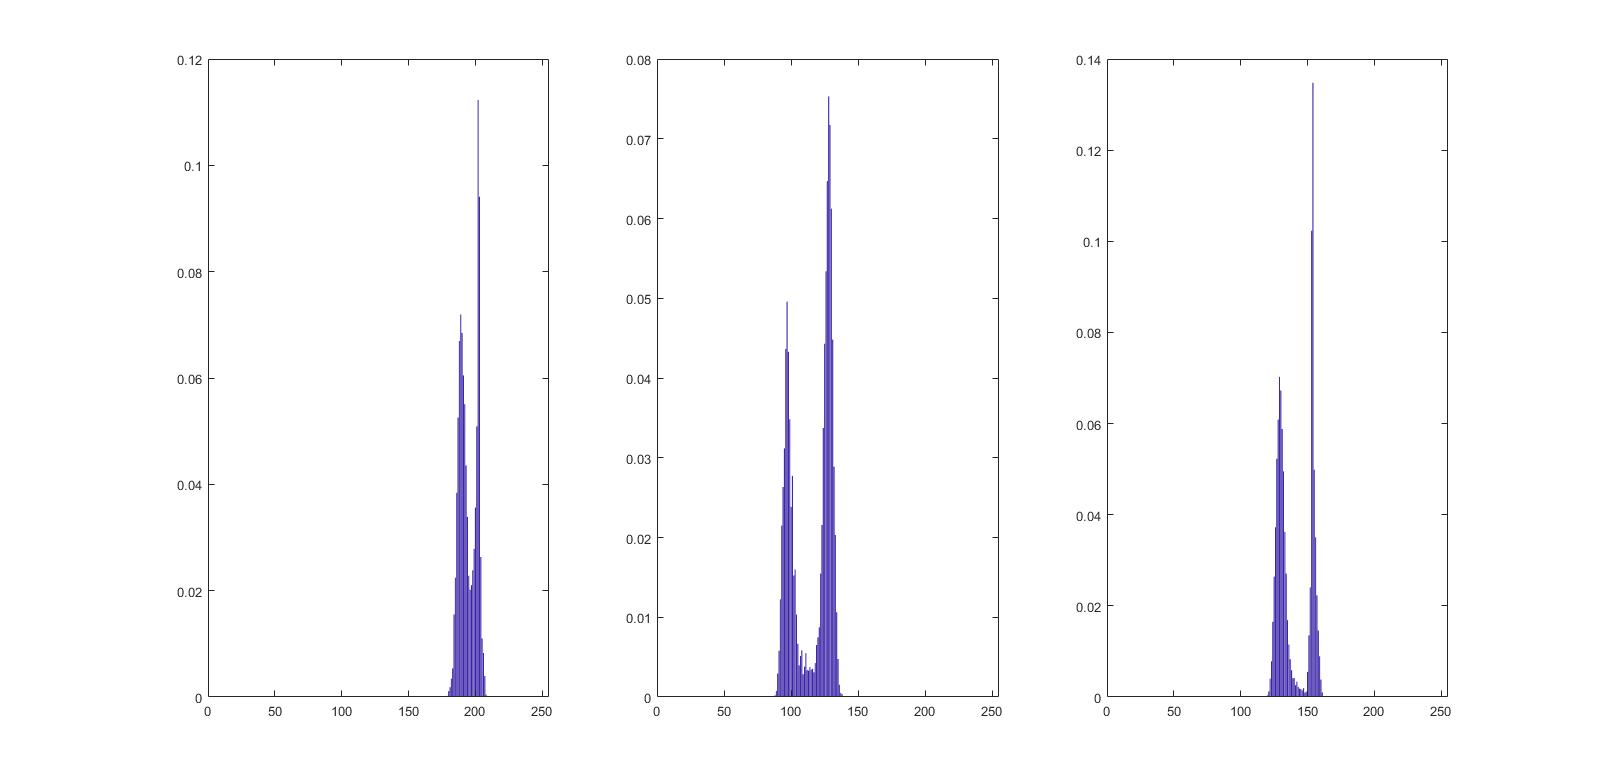
\includegraphics[width=0.9\textwidth]{ycbcr_hist3.jpg}
		\caption{}
		\label{fig:ycbcr_hist3}
	\end{subfigure}
	\caption{Obrazy i histogramy obszarów znacznika w~przestrzeni YCbCr.}
	\label{fig:histogramy_ycbcr}
\end{figure}
%TODO2 Super by było jakby jednak na rysunku pojawiły się obrazy wejściowe.(wykonane)

Zgodnie z~oczekiwaniami, zmiana poziomu oświetlenia przełożyła~się na~zmianę wartości luminancji, natomiast składowe chrominancji nie zmieniały się znacząco. 
Każdy z~obrazów może być skutecznie zbinaryzowany przy użyciu stałych progów: górnego 120 dla składowej Cb i~dolnego 150 dla składowej Cr. 
Różnice pomiędzy wartościami składowych dla znacznika i~tła nie są jednak duże -- wynoszą około 30 poziomów. 
Ostatecznie zdecydowano się na~znacznik przedstawiony na~rys. \ref{fig:znacznik}.
\begin{figure}[h]
	\centering
	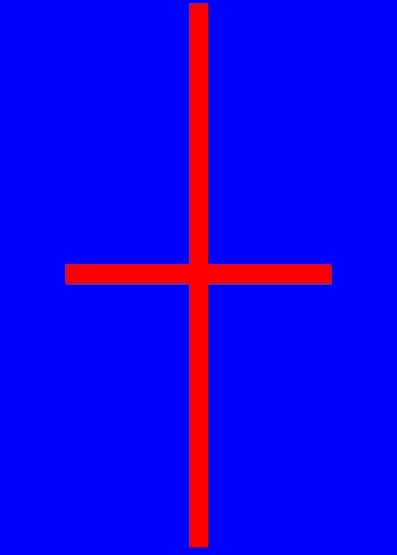
\includegraphics[width=0.3\textwidth]{znacznik.jpg}
	\caption{Wybrana postać znacznika}
	\label{fig:znacznik}
\end{figure}




\section{Analiza kąta widzenia kamery przy różnych ustawieniach rozdzielczości}
\label{sec:wyznaczenie_kata_widzenia_kamery_przy_roznych_ustawieniach}
W~celu zbadania kąta widzenia kamery stworzono moduł nakładający na~obraz prostopadłe linie przecinające się w~jego środku. %TODO2 to znowu odniesienie do tego rozdziału o SD (to było odczytane z monitora)
Następnie umieszczono kamerę na wysokości 49 cm i~skierowano ją w~dół. 
Odczytanie odległości od~środka obrazu do~jego krawędzi w~poziomie i~pionie pozwoliło na wyznaczenie kątów widzenia kamery. 
Skorzystano ze wzoru \eqref{eq:kat}.
\begin{equation}
\label{eq:kat}
\alpha=2\arctan{\frac{l}{h}}
\end{equation}
gdzie:
\begin{eqwhere}[2cm]
	\item[$\alpha$] kąt widzenia kamery,
	\item[$h$] wysokość, na jakiej umieszczona jest kamera,
	\item[$l$] odległość środka obrazu od jego krawędzi.
\end{eqwhere}
Na podstawie obrazu przedstawionego na rysunku \ref{fig:1080p} obliczono kąty widzenia kamery w~pionie i~poziomie dla rozdzielczości 1920 x 1080. 
Dla rozdzielczości 1280 x 720 skorzystano z~obrazu pokazanego na rysunku \ref{fig:720p}. 
Korzystając ze wzoru \eqref{eq:kat} otrzymano przybliżone wyniki, przedstawione w tabeli \ref{tab:rozdzielczosc}.
\begin{table}[]
	\caption{Wartości kąta widzenia kamery w zależności od rozdzielczości}
	\label{tab:rozdzielczosc}
	\centering
	\begin{tabular}{|c|c|c|}
		\hline
		\begin{tabular}[c]{@{}c@{}}Rozdzielczość\end{tabular} &  Kąt widzenia kamery w pionie w stopniach  &  Kąt widzenia kamery w poziomie w stopniach  \\ \hline
		1920 x 1080                                                                          & 28 & 54 \\ \hline
		1280 x 720                                                                         & 38 & 76 \\ \hline
	\end{tabular}
\end{table}

\begin{figure}
	\centering
	\begin{subfigure}{0.7\textwidth}
		\centering
		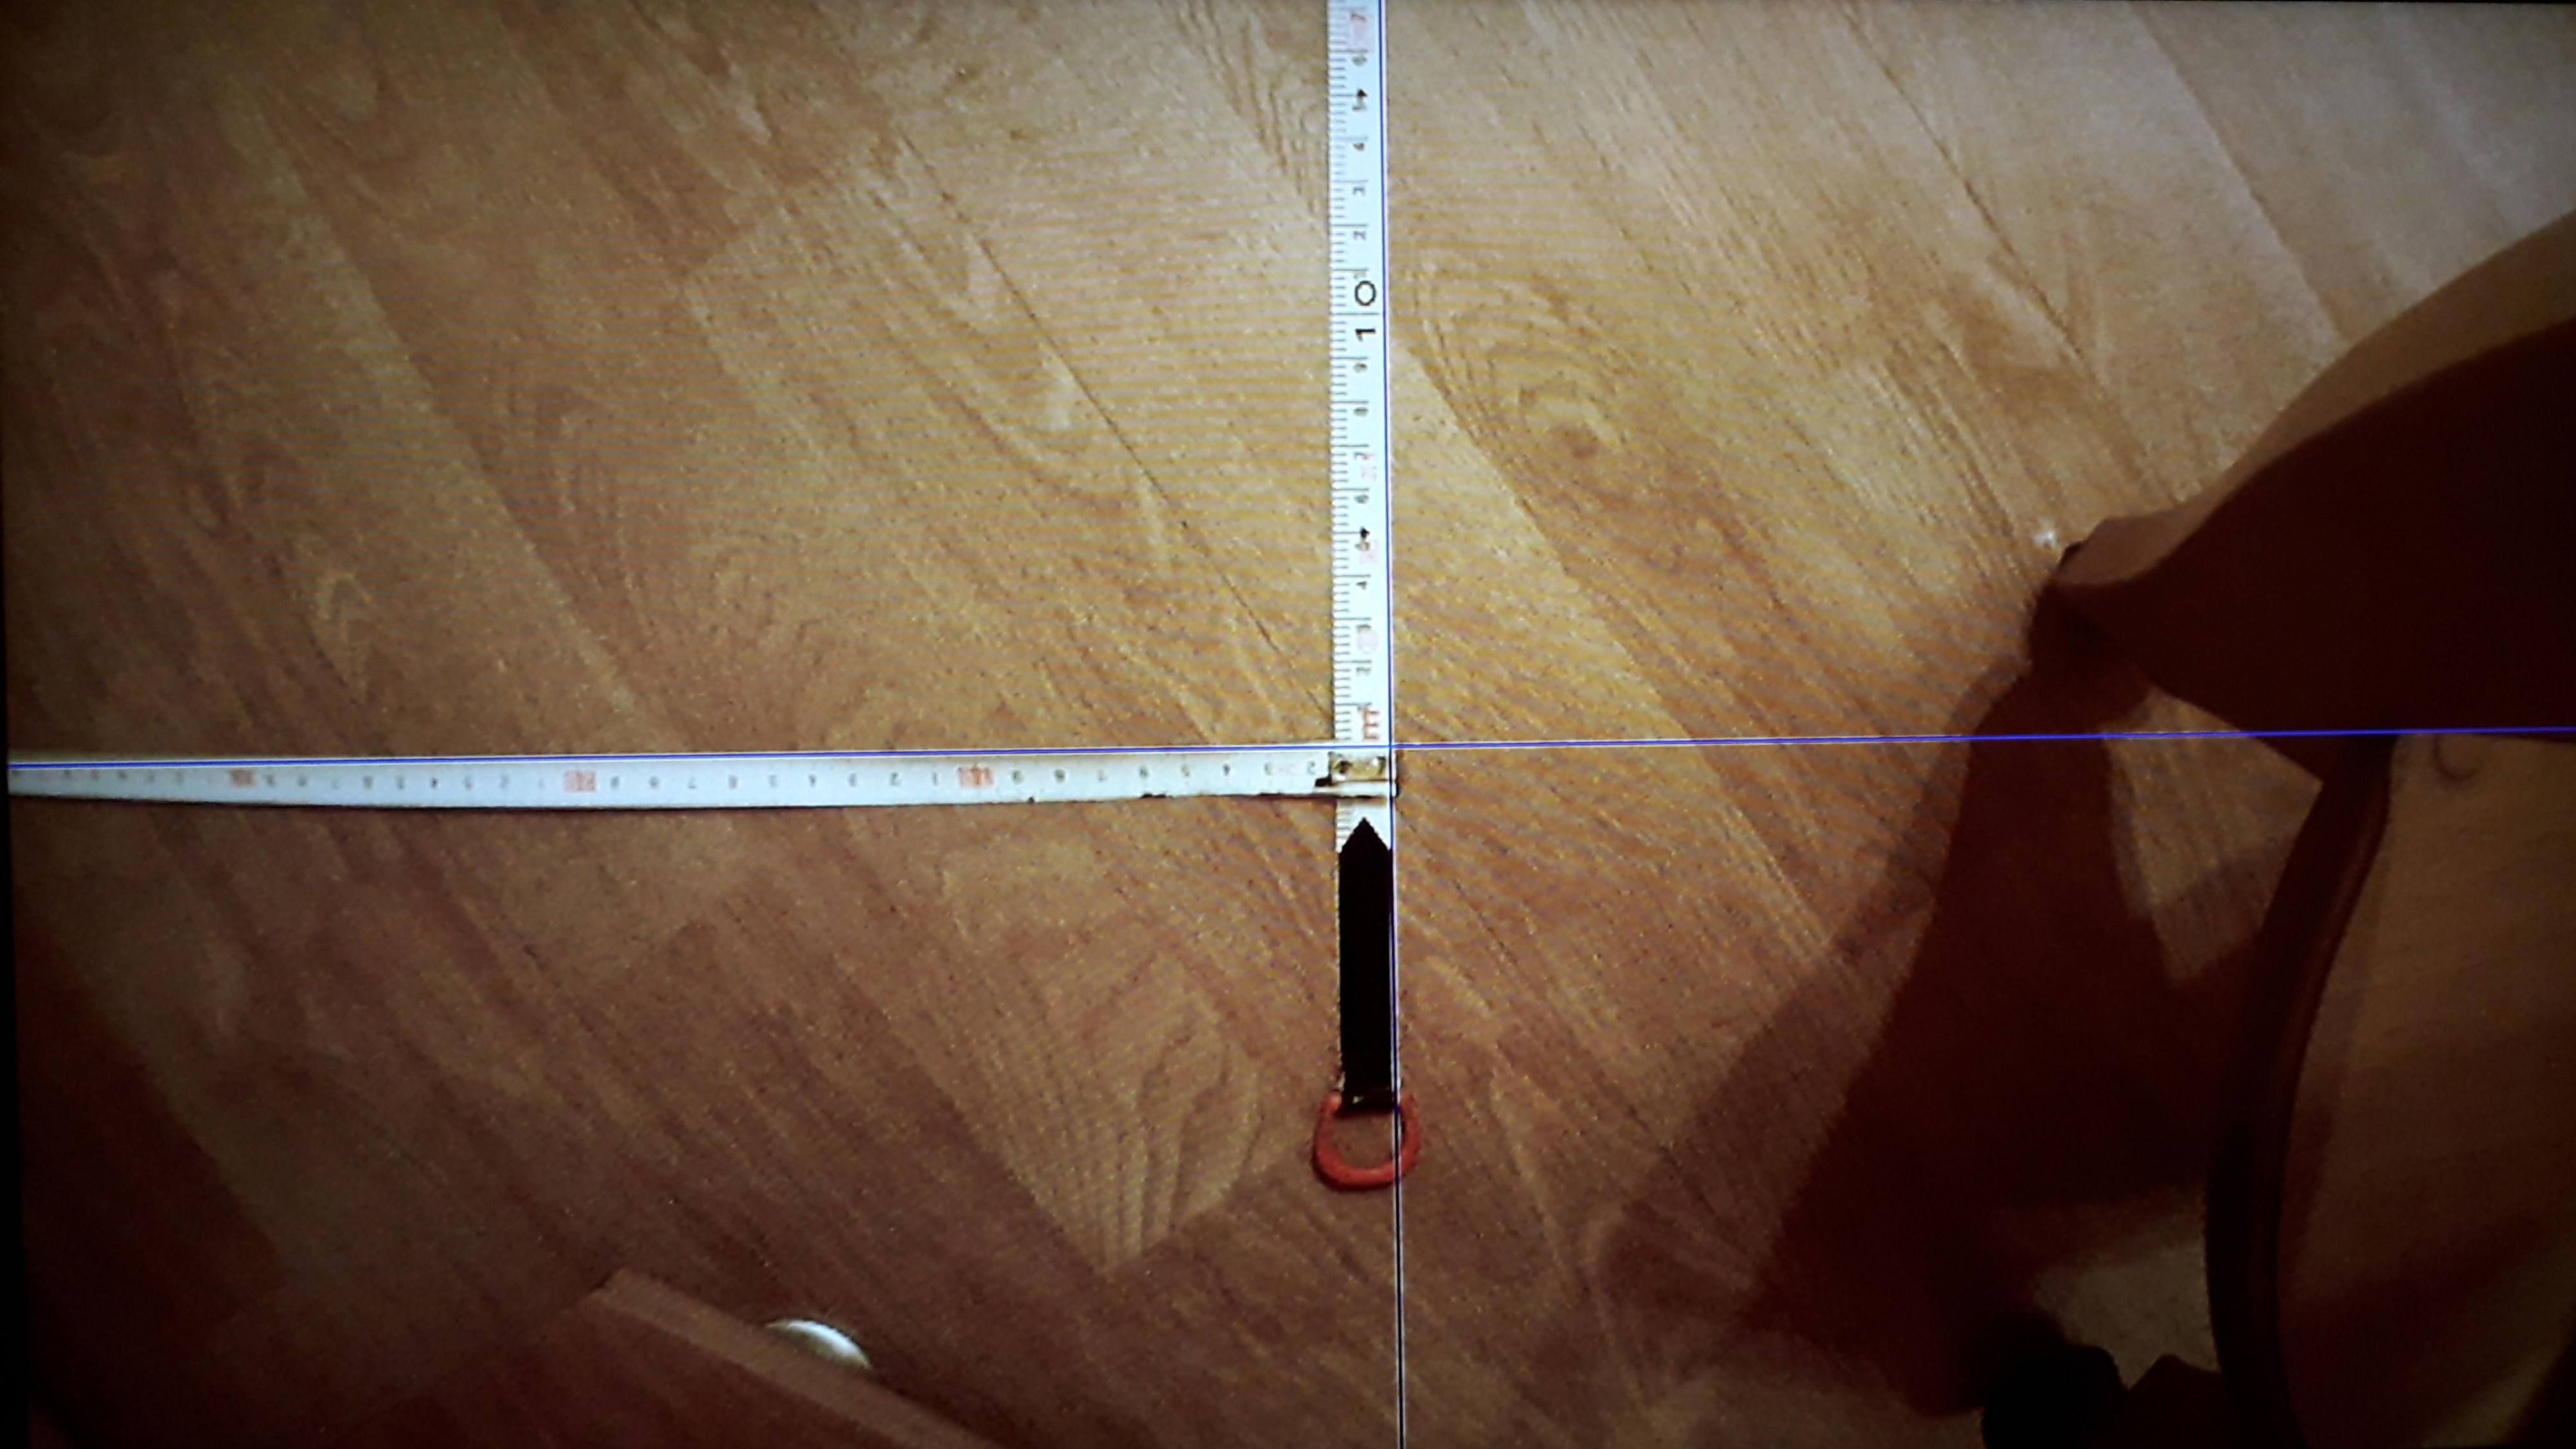
\includegraphics[width=0.9\textwidth]{720p.jpg}
		\caption{Rozdzielczość 1280 x 720.}
		\label{fig:1080p}
	\end{subfigure}
	\begin{subfigure}{0.7\textwidth}
		\centering
		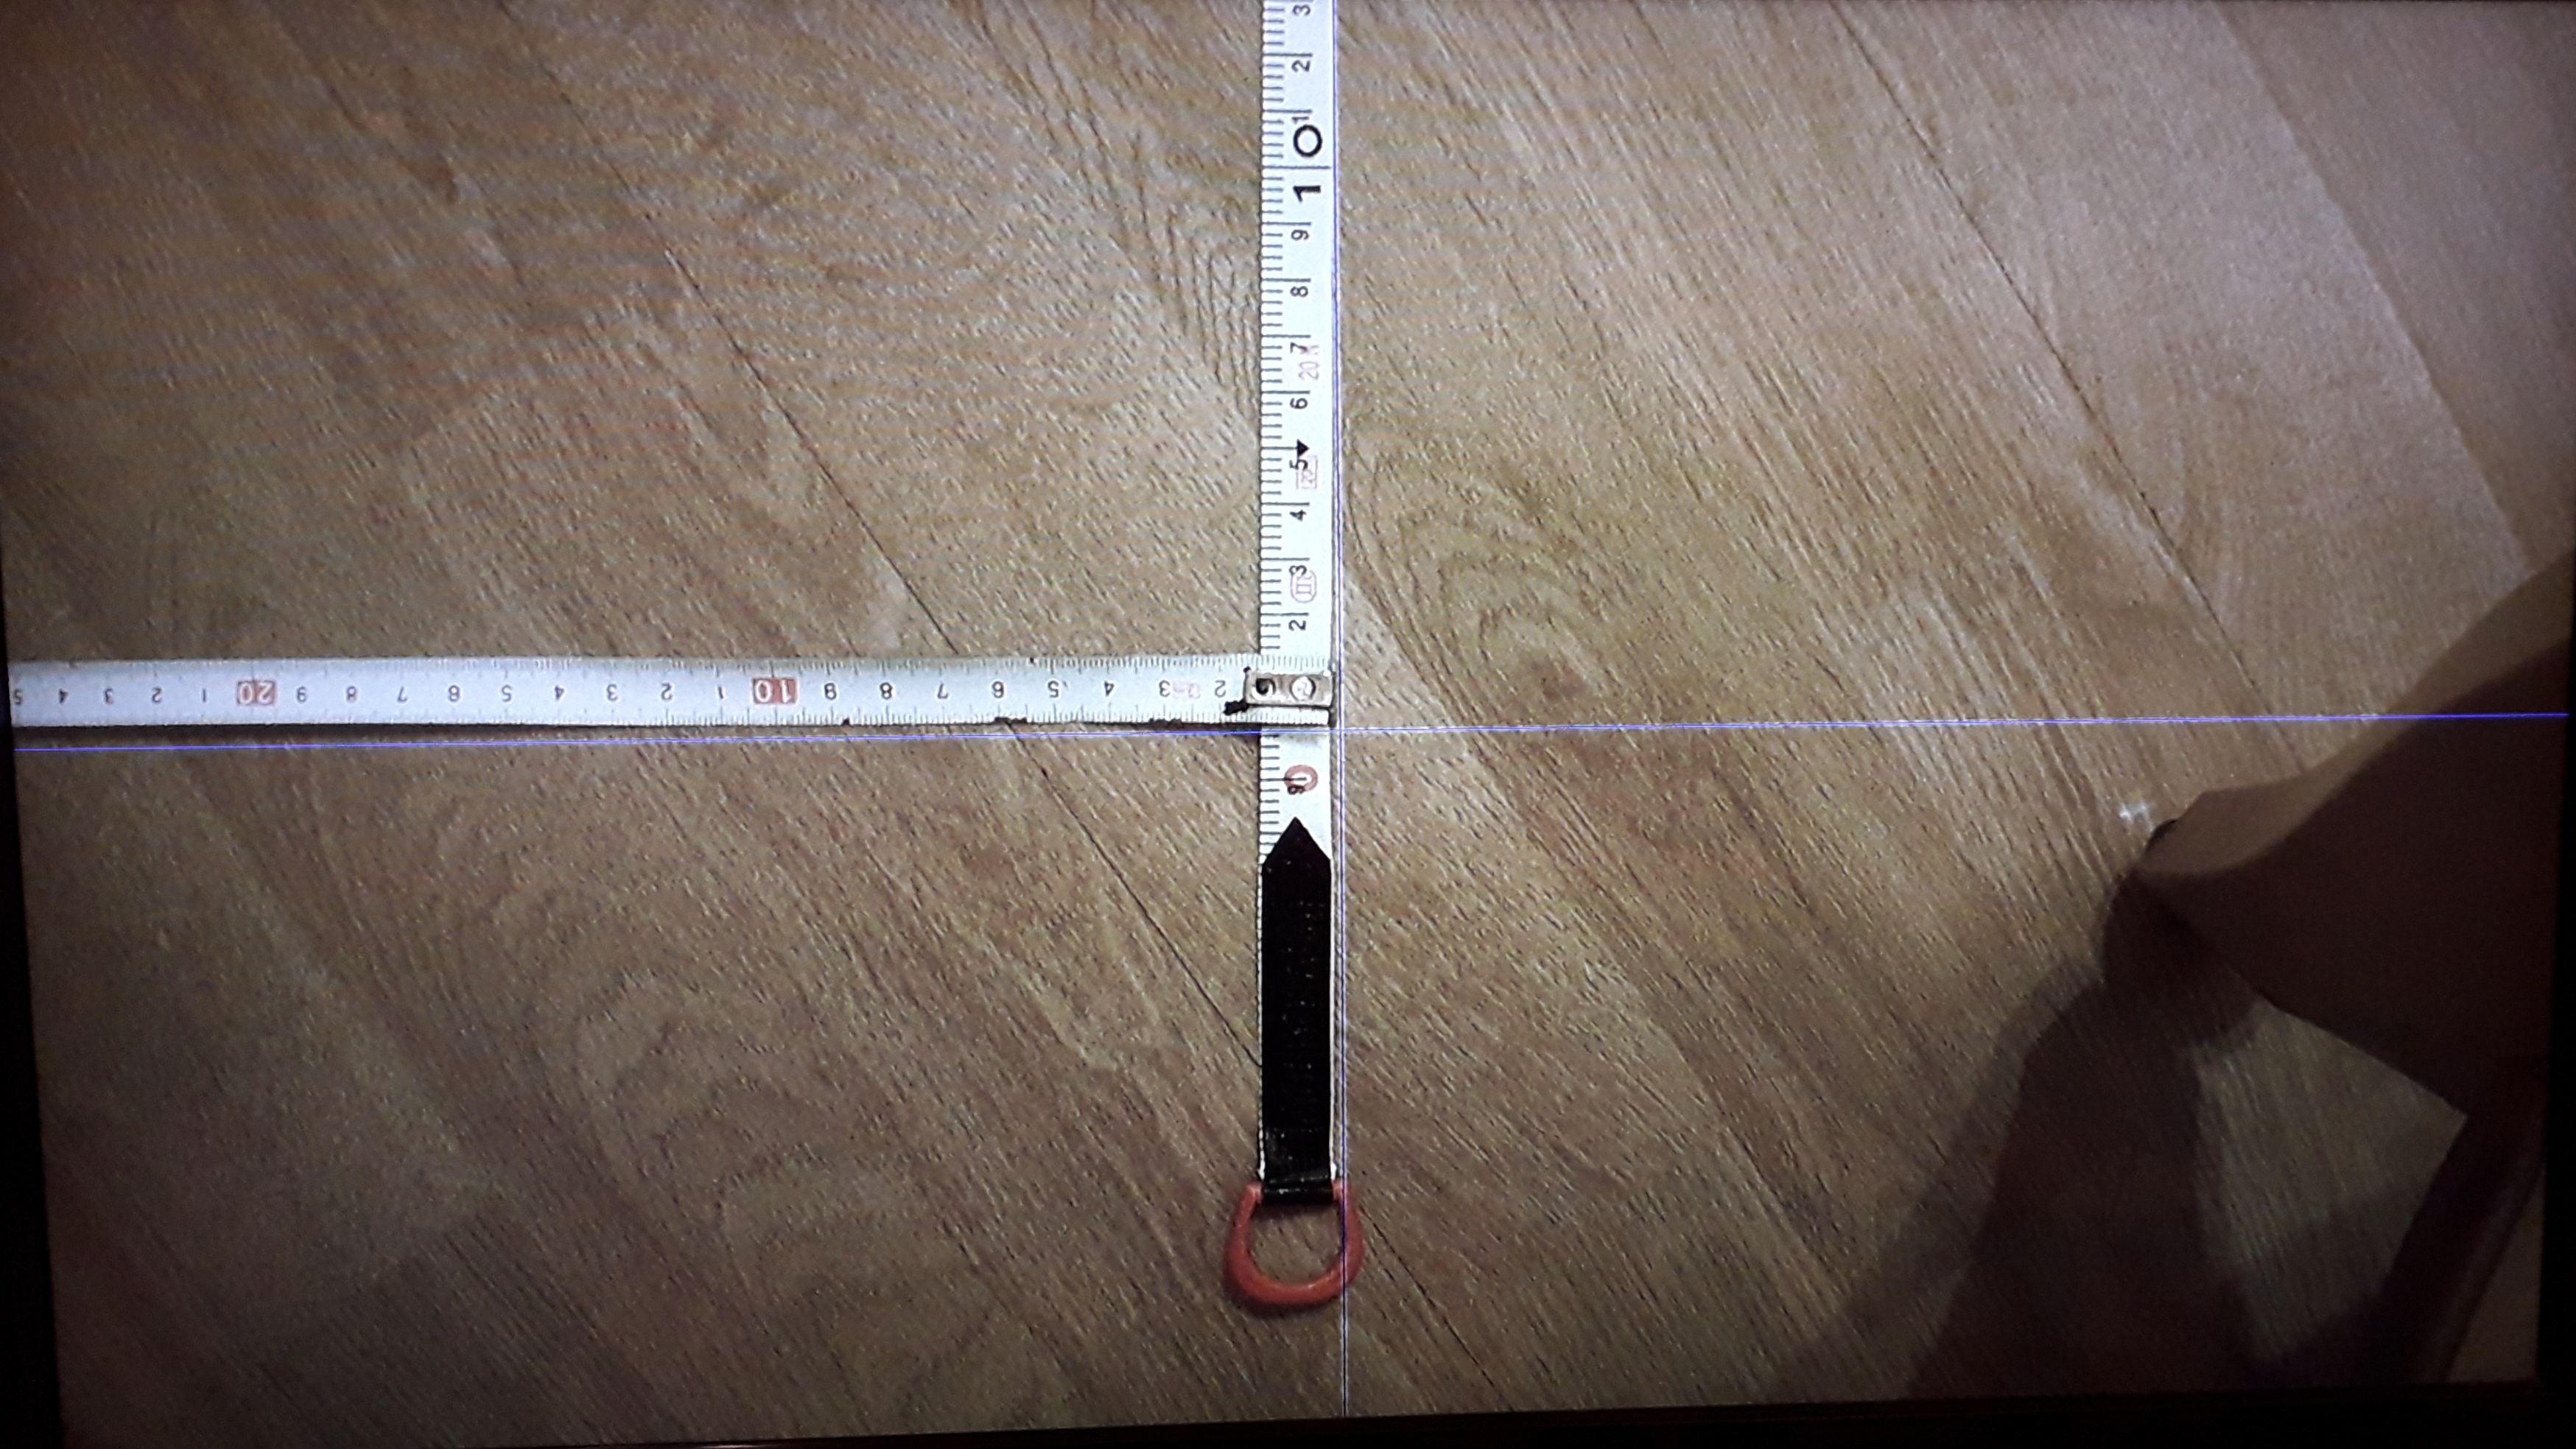
\includegraphics[width=0.9\textwidth]{1080p.jpg}
		\caption{Rozdzielczość 1920 x 1080.}
		\label{fig:720p}
	\end{subfigure}
	\caption{Obrazy służące do wyznaczenia kąta widzenia kamery.}
	\label{fig:rozdzielczosc}
\end{figure}
%TODO Jakieś wnioski...
Tak jak napisano w~podrozdziale \ref{sec:akwizycja}, dla rozdzielczości 1280~x~720 kąt widzenia kamery jest większy, co w~połączeniu z~mniejszą liczbą pikseli do~przetworzenia zdecydowało o~wyborze tej rozdzielczości.
Uzyskane wyniki oznaczają również, że~z~wysokości 1~m dron byłby w~stanie wykryć obiekty w~odległości 34~cm z~przodu i~z~tyłu, oraz 78~cm po~bokach.

\section{Podsumowanie}

%TODO Kilka zdań o tym modelu...
Implementacja modelu programowego umożliwiła przetestowanie działania poszczególnych modułów przetwarzania wizyjnego. Narzędzia programu Matlab okazały się również bardzo pomocne w~analizie koloru znacznika. Sprawdzenie kąta widzenia kamery pozwoliło zorientować się, z~jakiej odległości lądowisko będzie dla drona widoczne.

%TODO2 !!!! Bardzo nie lubię się potwarzać ! I jak dyplomant ignoruje moje uwagi ! To nie może tak być. Tu proszę przekopiować treść rozdziału testy - wybór znacznika i kąta widzenia. Ale nie tylko skopiować, ale też połączyć i uzupełnić zgodnie z uwagami. Natomiast w takim układzie implementacja sprzętowa + te dwa testy (bardziej sprzętowe) do nowego rozdziału (tzn. nowy \chapter). A ten "Test" znika !!!. I stosowana korekta treści we wstępie.




%TODO2 To co niżej to nowy rodział (chapter)
%TODO2 Proszę to jeszcze raz wszystko przeczytać !! Bo ja trochę poprzestawiałem....
\chapter{Implementacja i ewaluacja systemu sprzętowo-programowego}
\label{cha:implementacja_systemu}

Na rysunku \ref{fig:system} przedstawiono ogólny schemat zaimplementowanego systemu. 
Na~niebiesko zaznaczone zostały wykorzystywane urządzania, na~żółto oznaczono moduły zaimplementowane w~części rekonfigurowalnej, natomiast na~zielono zaznaczono system procesorowy. 
Sygnał wizyjny z~kamery trafia do~części reprogramowalnej i~jest następnie przetwarzany przez poszczególne moduły. 
Po~wyborze znacznika informacja o~jego pozycji i~uchybie regulacji trafia do~procesora. 
System procesorowy wysyła komendy sterujące do~kontrolera drona. 
Zadaniem układu regulacji jest przesunięcie drona nad~lądowisko, umożliwiając wykonanie lądowania.
W~dalszej części rozdziału omówiono poszczególne komponenty systemu. 

\begin{figure}[h]
	\centering
	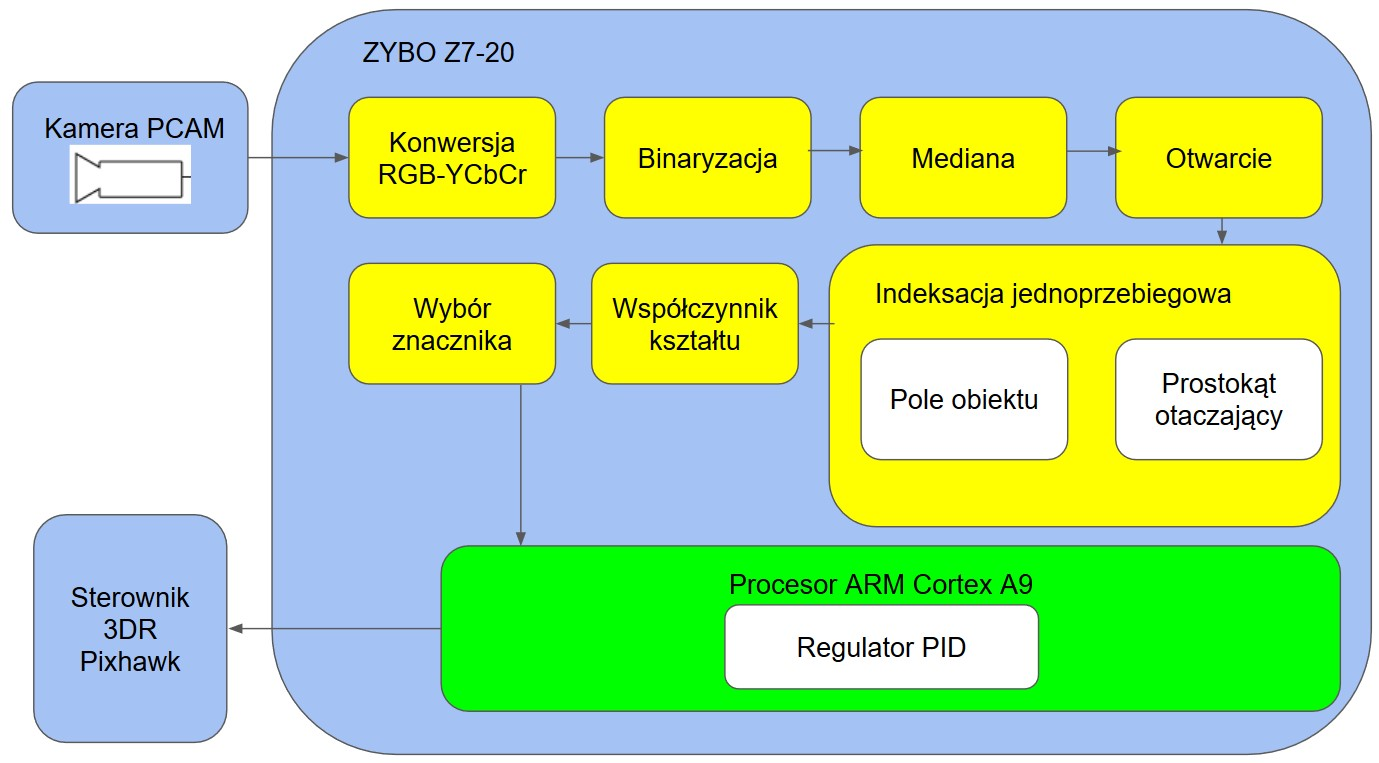
\includegraphics[width=\textwidth]{system.jpg}
	\caption{Schemat przedstawiający zaimplementowany system.}
	\label{fig:system}
\end{figure} 

\section{Akwizycja obrazu}
\label{sec:akwizycja}
Firma Digilent, na swojej stronie internetowej, zapewnia projekt demonstracyjny połączenia kamery i~płytki~\cite{projektPCAM}. 
Pozwala on pobrać obraz z~kamery oraz wyświetlić go na monitorze.
Ponadto, przez port szeregowy możliwa jest zmiana rozdzielczości, szybkości akwizycji ramek, współczynnika korekcji gamma oraz ustawień balansu bieli. 
Możliwe są~następujące opcje dotyczące dwóch pierwszych parametrów:
\begin{itemize}
	\item 1280 x 720, 60 fps,
	\item 1920 x 1080, 15 fps,
	\item 1920 x 1080, 30 fps.
\end{itemize}

Przeprowadzone eksperymenty pokazały, że przy rozdzielczości 1280 x 720 kąt widzenia kamery jest większy. 
Ze tego względu zdecydowano się użyć tej rozdzielczości w~docelowym systemie.
Przeprowadzanie syntezy i~implementacji projektu możliwe było przy użyciu darmowego oprogramowania Vivado oraz SDK w~wersji WebPack (w wersji~2018.2). 
Opisany projekt stanowił bazę do dalszych prac.

\subsection{Zapis ramek na kartę SD}
\label{sec:image_sd}
%TODO2 Do tego ma się znaleźć link w tej części o modelu !!!(wykonane)
Aby możliwe było użycie ramek z kamery w~modelu programowym, należało zaimplementować akwizycję obrazów na~kartę~SD. 
W~użytym projekcie bazowym zastosowano połączenie toru wizyjnego AXI z~zewnętrzną pamięcią RAM dostępną na karcie Zybo poprzez moduł \textit{AXI Video Direct Memory Access}. 
%Informacja o~adresie pamięci, gdzie zapisywane są~ramki, podawana jest przy inicjalizacji połączenia na~terminal. 
%TODO2 to jest niejasne.(poprawione poniżej)
Szesnastkowy adres miejsca w~pamięci, gdzie znajduje się wartość składowej R pierwszego piksela ramki, przesyłany jest do~użytkownika przy inicjalizacji połaczenia. Możliwe jest jego odczytanie i~dotarcie do~zawartości pamięci przy wykorzystaniu wskaźnika w~języku~C++.

W~celu umożliwienia komunikacji z~kartą SD uaktywniono interfejs procesora SD0. 
Następnie do~projektu w~SDK dodano bibliotekę ,,xilffs'' i~korzystając z~funkcji systemu plików opisanych w~\cite{xilffs}, zaimplementowano zapis ramek obrazu do~pliku. 
Ze~względu na~prostotę pliku zdecydowano~się na~format ppm. 
W~formacie tym nie występuje kompresja i~przez to jest on~nieefektywny pod~względem zapotrzebowania na pamięć.
Niemniej jednak, dysponując odpowiednio dużą ilością miejsca na~karcie i~chcąc w~łatwy sposób zapisać dane, warto zastosować właśnie ten format. 
Zapis danych w~formacie ppm jest prosty, gdyż plik składa się jedynie z~nagłówka (typ pliku, rozmiary obrazka, maksymalna wartość składowych) oraz kolejnych wartości w~formie pojedynczych bajtów (jeśli maksymalna wartość jest mniejsza niż 256).  



\section{Podłączenie laserowego czujnika wysokości}
\label{subsec:podlaczenie_lasera}

Czujnik wysokości podłączono z~zastosowaniem wyjścia PWM (ang. \textit{Pulse-Width Modulation}). %TODO2 a) rozwinąć skrót, b) w opisie sprzętu zaznaczyć, że są dwie możliwości (wykonane)
W~tym trybie czujnik ustawia stan wysoki na~wyjściu przez czas proporcjonalny do~zmierzonej odległości. 
Stan wysoki trwa 10~\si{\micro\second} na~każdy zmierzony centymetr. 
Pin wyzwalania zwarto na~stałe do~masy, powodując ciągłe wykonywanie pomiaru. 
Wyjście PWM podłączono do~trzeciego pinu portu Pmod~JB układu ZYBO. %TODO2 skoro tak, to znowu w opisie sprzętu trzeba zaznaczyć, co to jest PMod (wykonane)
Okazało się, że~możliwe jest działanie modułu przy zasilaniu bezpośrednio z~płytki z napięciem 3,3~V.

Moduł odczytujący wysokość zaimplementowany został jako maszyna stanów. 
Stan pierwszy to~oczekiwanie na~pojawienie się stanu wysokiego. 
Po~wykryciu zbocza narastającego następuje zerowanie rejestrów oraz przejście do~stanu drugiego. 
W~tym stanie liczony jest czas trwania stanu wysokiego. 
Wywoływanie procesu z~częstotliwością 1~MHz, czyli co~1~\si{\micro\second} pozwala na~łatwą konwersję zmierzonego czasu na~odległość. 
Odczytana wysokość jest następnie przesyłana do~procesora z~użyciem rejestrów~AXI.


\section{Konwersja z przestrzeni barw RGB do YCbCr}
\label{subsec:konwersja}
Konwersję z przestrzeni barw RGB do YCbCr wykonano zgodnie ze wzorem \ref{eq:ycbcr}. 
Przy implementacji wykorzystano sprzętowe mnożarki oraz sumatory. 
Na~rysunku \ref{fig:drzewo_ycbcr} przedstawiono schemat operacji arytmetycznych dla jednej ze~składowych. 
Aby możliwe było prowadzenie obliczeń, wszystkie stałe należało przedstawić w~postaci liczb stałoprzecinkowych. 
Do~reprezentacji stałoprzecinkowej użyto rejestrów o~szerokości 18~bitów.
\begin{equation}
\label{eq:ycbcr}
\begin{bmatrix} Y \\ 
Cb\\
Cr
\end{bmatrix}=
\begin{bmatrix} 0,299 & 0,587 & 0,114\\ 
-0,168736 & -0,331264 & 0,5\\
0,5 & -0,418688 & 0,081312
\end{bmatrix}
\begin{bmatrix} R\\
G\\
B
\end{bmatrix}+
\begin{bmatrix} 0\\
128\\
128
\end{bmatrix}
\end{equation}


\begin{figure}[h]
	\centering
	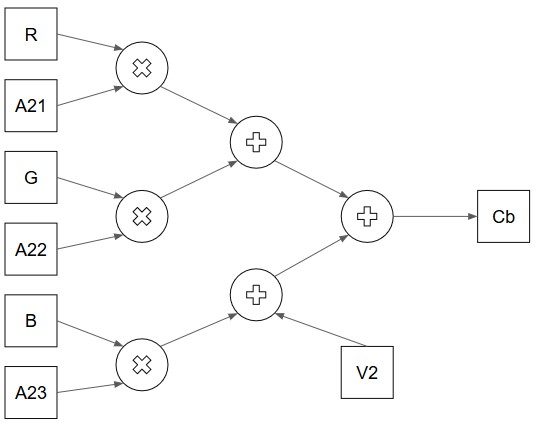
\includegraphics[width=0.7\textwidth]{drzewo_ycbcr.jpg}
	\caption{Schemat wyznaczania składowej Cb. $A21=-0,168736, A22=-0,331264, A23=0,5, V2=128$.}
	\label{fig:drzewo_ycbcr}
\end{figure} 

\section{Binaryzacja}
\label{subsec:Binaryzacja}
% dobieranie progu: 2 multiplekser sterowany buttonem?
Piksel wyjściowy otrzymywał wartość maksymalną (kolor biały), jeśli wartości Cb i~Cr mieściły się pomiędzy wyznaczonymi eksperymentalnie progami.  
W~innym przypadku pikselowi przypisywana była wartość 0 (kolor czarny). 
Do~szybkiej zmiany progów wykorzystano komunikację PS-PL z~użyciem rejestrów AXI -- progi mogły być zmieniane z~poziomu terminala i~testy nie wymagały ponownych implementacji projektu.  


\section{Mediana}
\label{subsec:Mediana}
% obrazek wyznaczania kontekstu
% obrazek drzewa sumacyjnego

W~przypadku działania na~obrazie binarnym operacja mediany może być przeprowadzona przez obliczenie sumy wartości pikseli wewnątrz kontekstu, a~następnie porównanie jej z~połową maksymalnej wartości tej sumy. 
Ze względu na łatwość implementacji oraz zadowalające wyniki filtracji, zdecydowano się na~rozpatrywanie kontekstu w~kształcie kwadratu o~boku 5~pikseli. 
Spowodowało to~konieczność zapamiętywania kontekstu piksela w~25 rejestrach oraz 4~linii obrazu w~długich liniach opóźniających zbudowanych w~oparciu o~pamięć BRAM.
Schemat wyznaczania kontekstu przedstawiono na rysunku \ref{fig:kontekst}. 
Sygnały synchronizacji zostały doklejone do wartości piksela i~w~przedstawionej strukturze przesuwają się razem z~nim. 
Sumę wyliczano w~2~etapach, dodając najpierw elementy w~wierszach, potem sumując wyniki (Rys. \ref{fig:drzewo_sumacyjne}).

\begin{figure}[h]
	\centering
	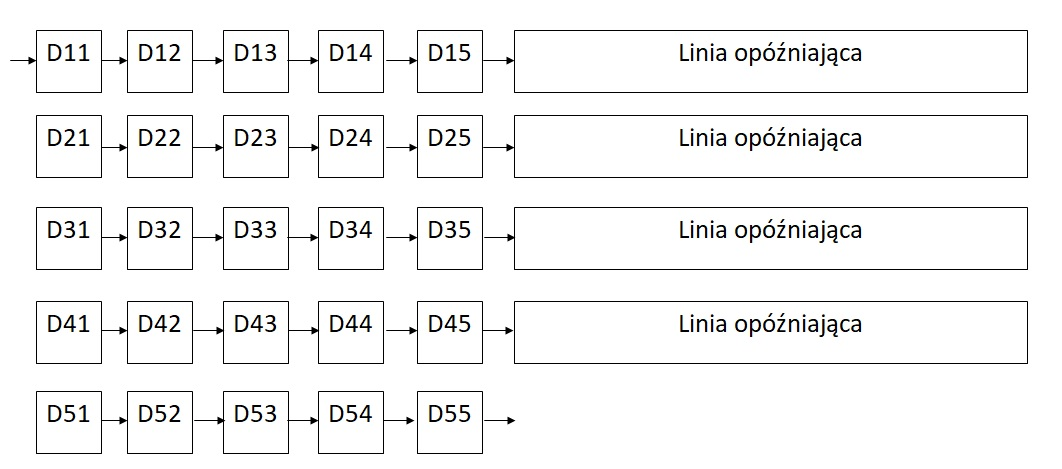
\includegraphics[width=0.8\textwidth]{kontekst.jpg}
	\caption{Schemat wyznaczania kontekstu dla mediany, erozji i dylatacji.}
	\label{fig:kontekst}
	%TODO2 nieco mniejszy ten rysunek (wykonane)
\end{figure}  

\begin{figure}[h]
	\centering
	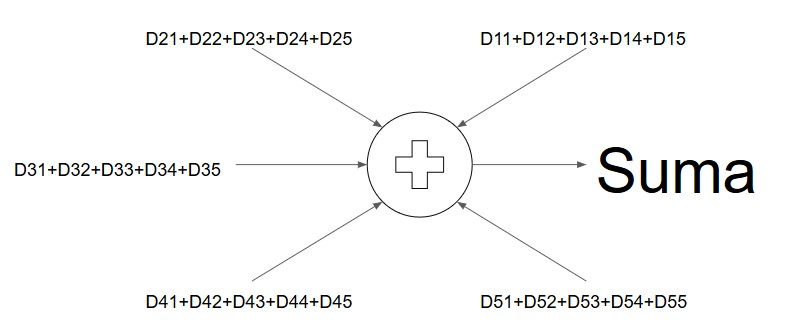
\includegraphics[width=\textwidth]{drzewo_sumacyjne.jpg}
	\caption{Schemat wyznaczania sumy otoczenia piksela.}
	\label{fig:drzewo_sumacyjne}
\end{figure}  

\subsection{Otwarcie}
\label{subsec:erozja}

Moduł erozji ustawia wartość piksela wyjściowego na~maksymalną wartość, gdy~w~sąsiedztwie znajdują się same białe piksele. 
W~module dylatacji zwracana jest wartość maksymalna, gdy~przynajmniej jeden piksel w~sąsiedztwie ma~wartość maksymalną.
Podobnie jak w~przypadku mediany, jako element strukturalny zdecydowano się na~kwadrat o~boku 5~pikseli i~zastosowano rozwiązanie podobne jak przy medianie (Rys. \ref{fig:kontekst}).
%TODO2 Tu jakieś zdanie, że zostaosowano podobne rozwiązanie jak przy medianie (wykonane)

%TODO2 Teraz patrząc na schemat to indeksacja.
\subsection{Indeksacja}
\label{subsec:indeksacja}

Zazwyczaj na wejście modułu indeksacji podawany jest obraz zbinaryzowany, natomiast na~wyjściu pojawia się obraz, na którym  wartość  pikseli odpowiada przypisanej do~danego obiektu etykiecie. 
Rozważane jest otoczenie każdego piksela, składające się z trzech pikseli nad nim oraz jednego po~lewej stronie, tak jak zostało to przedstawione na rysunku \ref{fig:ind_sasiedztwo}. 
Indeksacji dokonuje się bezpośrednio na~obrazie wejściowym. 
Podczas iteracji po wszystkich pikselach, w~przypadku znalezienia piksela należącego do któregoś z~obiektów, może zajść jeden z~trzech przypadków:
\begin{enumerate}[label=(\alph*)]
	\item w~otoczeniu piksela znajdują się tylko piksele należące do tła,
	\item otoczenie zawiera jeden lub więcej pikseli, którym została wcześniej przypisana taka sama etykieta~$L$,
	\item w~otoczeniu znajdują się piksele posiadające różne etykiety (np. $L1$ i $L2$).
\end{enumerate} 
\begin{figure}[h]
	\centering
	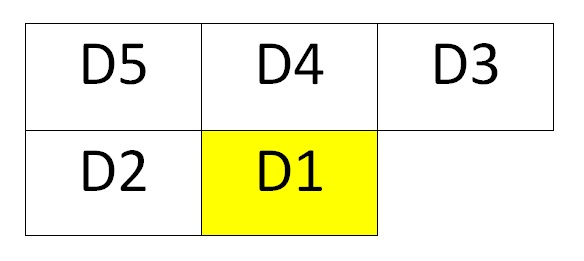
\includegraphics[width=0.5\textwidth]{ind_sasiedztwo.jpg}
	\caption{Sąsiedztwo piksela brane pod uwagę przy indeksacji}
	\label{fig:ind_sasiedztwo}
\end{figure}

W~pierwszym przypadku pikselowi zostaje przypisana nowa etykieta. 
Gdy spełniony jest warunek $b$, punkt otrzymuje etykietę $L$, natomiast jeśli zachodzi przypadek $c$, przypisywana jest mniejsza z~etykiet. 
W~ten sposób otrzymuje się obraz wstępnie poetykietowany. 
Najczęściej posiada on więcej przypisanych etykiet, niż obiektów. 
Dlatego istnieje konieczność złączenia ze~sobą pewnych etykiet przy użyciu tablicy sklejeń. 
Tablica ta zawiera informację, które etykiety powinny zostać złączone. 
W~przypadku~$a$ do tablicy sklejeń na~pozycji odpowiadającej etykiecie zapisywana jest etykieta, natomiast gdy zachodzi opcja~$c$ etykietę mniejszą zapisuje się pod indeksem większej. 
Należy zaznaczyć, że opisana wersja obsługi sklejeń działa poprawnie tylko w~przypadku braku tzw. ,,łańcuchów sklejeń'' tj. dla uproszczonych kształtów. %TODO2 Proszę mieć tego świadomość !
Do sklejenia etykiet potrzebna jest druga iteracja, tym razem po~obrazie wstępnie poetykietowanym.

Powyższy fakt jest główną przeszkodą w~łatwym wykonaniu takiego algorytmu w~systemie potokowym. 
Bez~zapamiętywania całej ramki, w~przypadku sklejania etykiet, niemożliwy jest powrót do~wcześniej przetwarzanych pikseli. 
Pomimo tego, możliwe jest obliczenie pewnych cech obiektów, takich jak: pole, współrzędne środka ciężkości, prostokąt otaczający. 
W~pracy \cite{COG} podano sposób, w~jaki można tego dokonać. 
Opiera się on~na~scaleniu nie samych wartości pikseli, ale~obliczanych na~bieżąco parametrów obiektu.
Implementacja indeksacji w~języku Verilog rodzi trudności związane z~określeniem przypadku istnienia tej~samej lub~różnych etykiet w~otoczeniu piksela. 

O~ile~wykrycie przypadku $a$ jest łatwe, to~przypadki $b$~i~$c$ wymagały rozważenia kilku możliwości. 
Zdecydowano się na~wykrywanie ich za~pomocą flag bitowych. 
Na~ich podstawie wnioskowano o~zachodzącym aktualnie przypadku oraz wskazywano, od~którego piksela z~otoczenia powinna zostać przepisana etykieta. 
Zgodnie z~opisanymi wcześniej zasadami uzupełniano również tablicę sklejeń.
Oprócz tego, na bieżąco obliczano prostokąt otaczający oraz liczbę pikseli należących do~każdego ze~znalezionych obiektów. 


Po poetykietowaniu całej ramki obrazu wykorzystano tablicę sklejeń do~złączenia obliczanych na~bieżąco cech. 
Ten~etap algorytmu zaimplementowano jako maszynę stanów:
\begin{itemize}
	\item Stan 0 -- Oczekiwanie na sygnał końca ramki wyznaczany na podstawie synchronizacji pionowej. W~momencie wykrycia sygnału następuje rejestrowanie tablicy sklejeń i~obliczonych parametrów (w~następnym takcie zostaną one zresetowane), zerowanie tablic wypełnianych w~kolejnym etapie oraz przejście do~stanu~1. 
	\item Stan 1 -- Iteracja po tablicy sklejeń i~uzupełnianie rzeczywistych wartości cech obiektów.
	\item Stan 2 -- Uporządkowanie tablic z~wyznaczonymi parametrami.
	\item Stan 3 -- Obliczenie pola prostokąta otaczającego dla każdego znalezionego obiektu. Wykorzystywana jest mnożarka o~latencji 3.
	\item Stan 4 -- Szukanie obiektu spełniającego warunki minimalnej wielkości pola powierzchni oraz stosunku pola prostokąta otaczającego do pola obiektu.
\end{itemize}
Schemat przetwarzania danych po~każdej ramce pokazano na rysunku \ref{fig:ind_schemat}.
\begin{figure}[h]
	\centering
	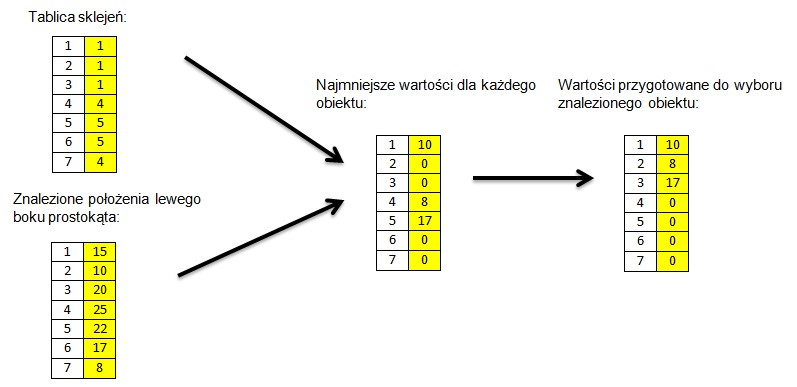
\includegraphics[width=\textwidth]{ind_schemat.jpg}
	\caption{Schemat procesu przetwarzania informacji po~każdej ramce obrazu przy zastosowaniu indeksacji z~przykładowymi danymi. Tablica sklejeń daje informację o~konieczności sklejenia etykiet 1, 2, 3. Ponieważ przykład dotyczy lewego boku prostokąta, spośród liczb 15, 10, 20 (odpowiadającym etykietom 1, 2, 3) wybierana jest najmniejsza. Ostatni krok przetwarzania to~usunięcie środkowych zer z~wektora.}
	\label{fig:ind_schemat}
\end{figure}


Główną trudnością w~implementacji opisanego algorytmu w~układzie FPGA jest stosunkowo duże zapotrzebowanie na~zasoby sprzętowe. 
Należy zarezerwować miejsce na~cechy każdego potencjalnego obiektu. 
Ogranicza to~liczbę możliwych etykiet. 
Zasoby części rekonfigurowalnej układu dostępnego na karcie ZYBO~Z7-20 pozwoliły na~zarezerwowanie miejsca dla~30~etykiet. 
Przy pewnej określonej orientacji znacznika nie jest to~niestety wystarczająca liczba etykiet (Rys. \ref{fig:rezultaty_ind}). %TODO2 może przykład (zdjęcie) i komentarz 
\begin{figure}
	\centering
	\begin{subfigure}{0.45\textwidth}
		\centering
		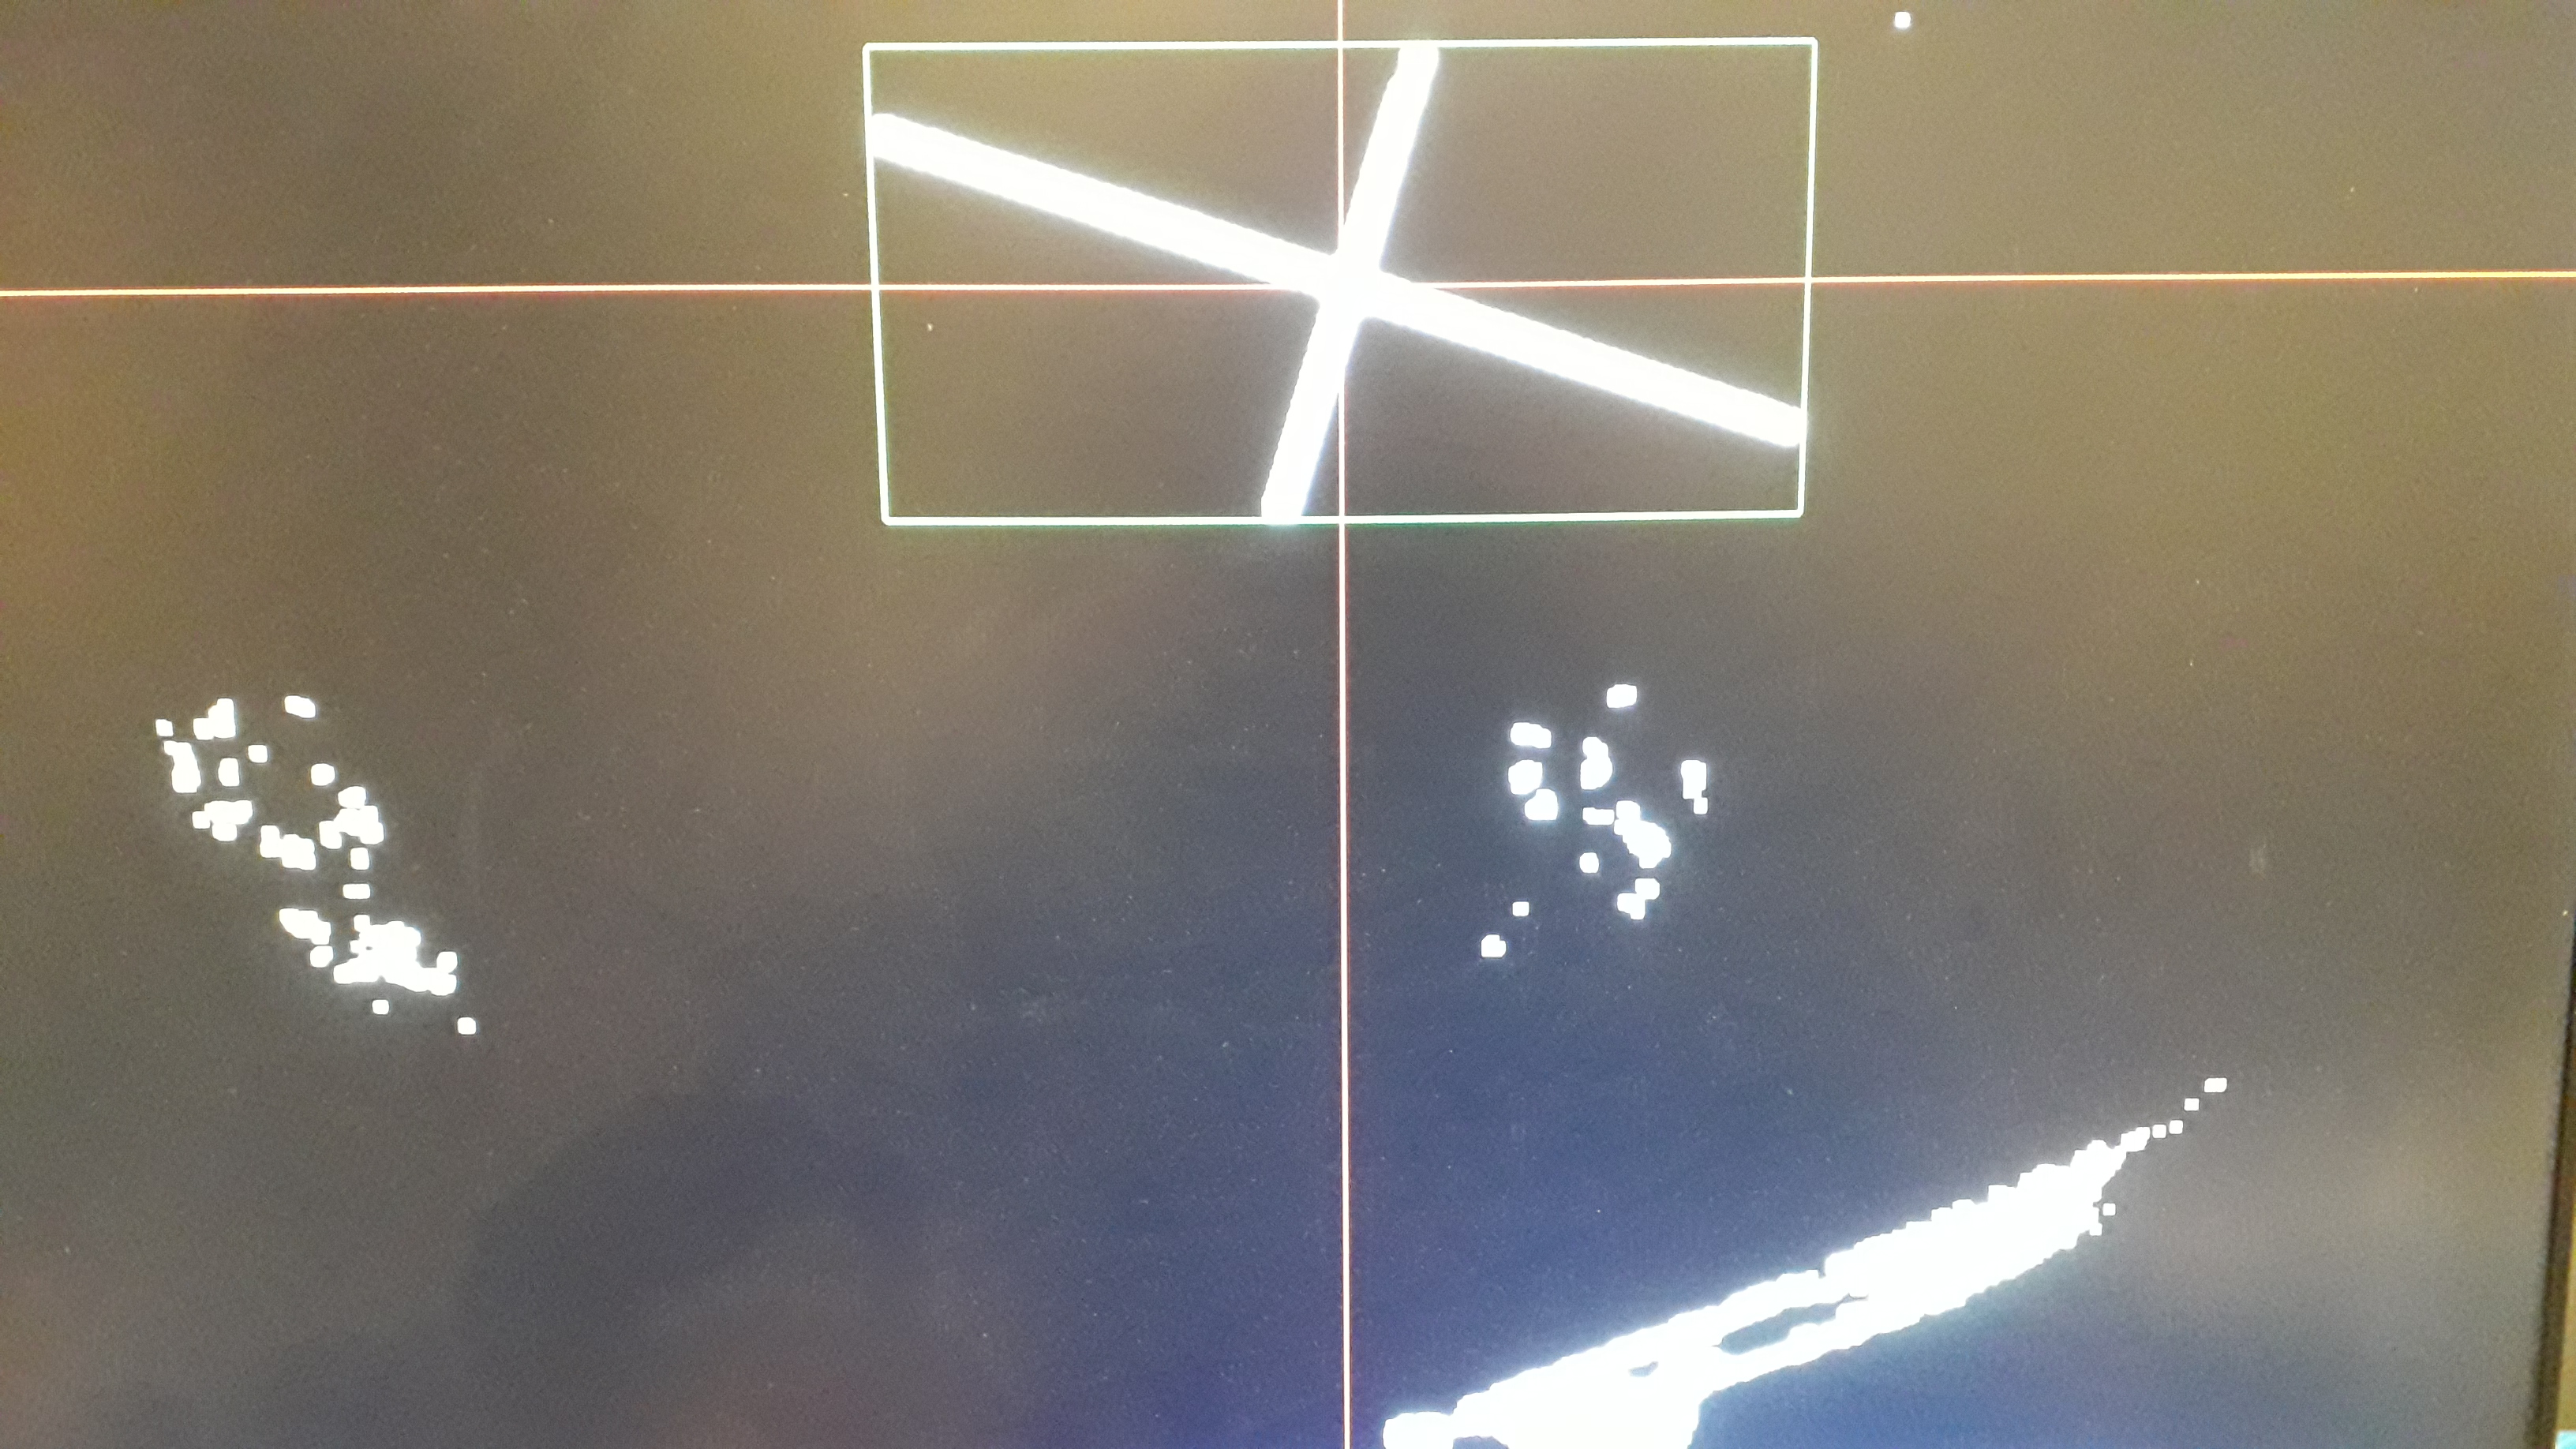
\includegraphics[width=\textwidth]{ind_poprawna.jpg}
		\caption{Poprawne wykrycie znacznika}
		\label{fig:ind_poprawna}
	\end{subfigure}
	\begin{subfigure}{0.45\textwidth}
		\centering
		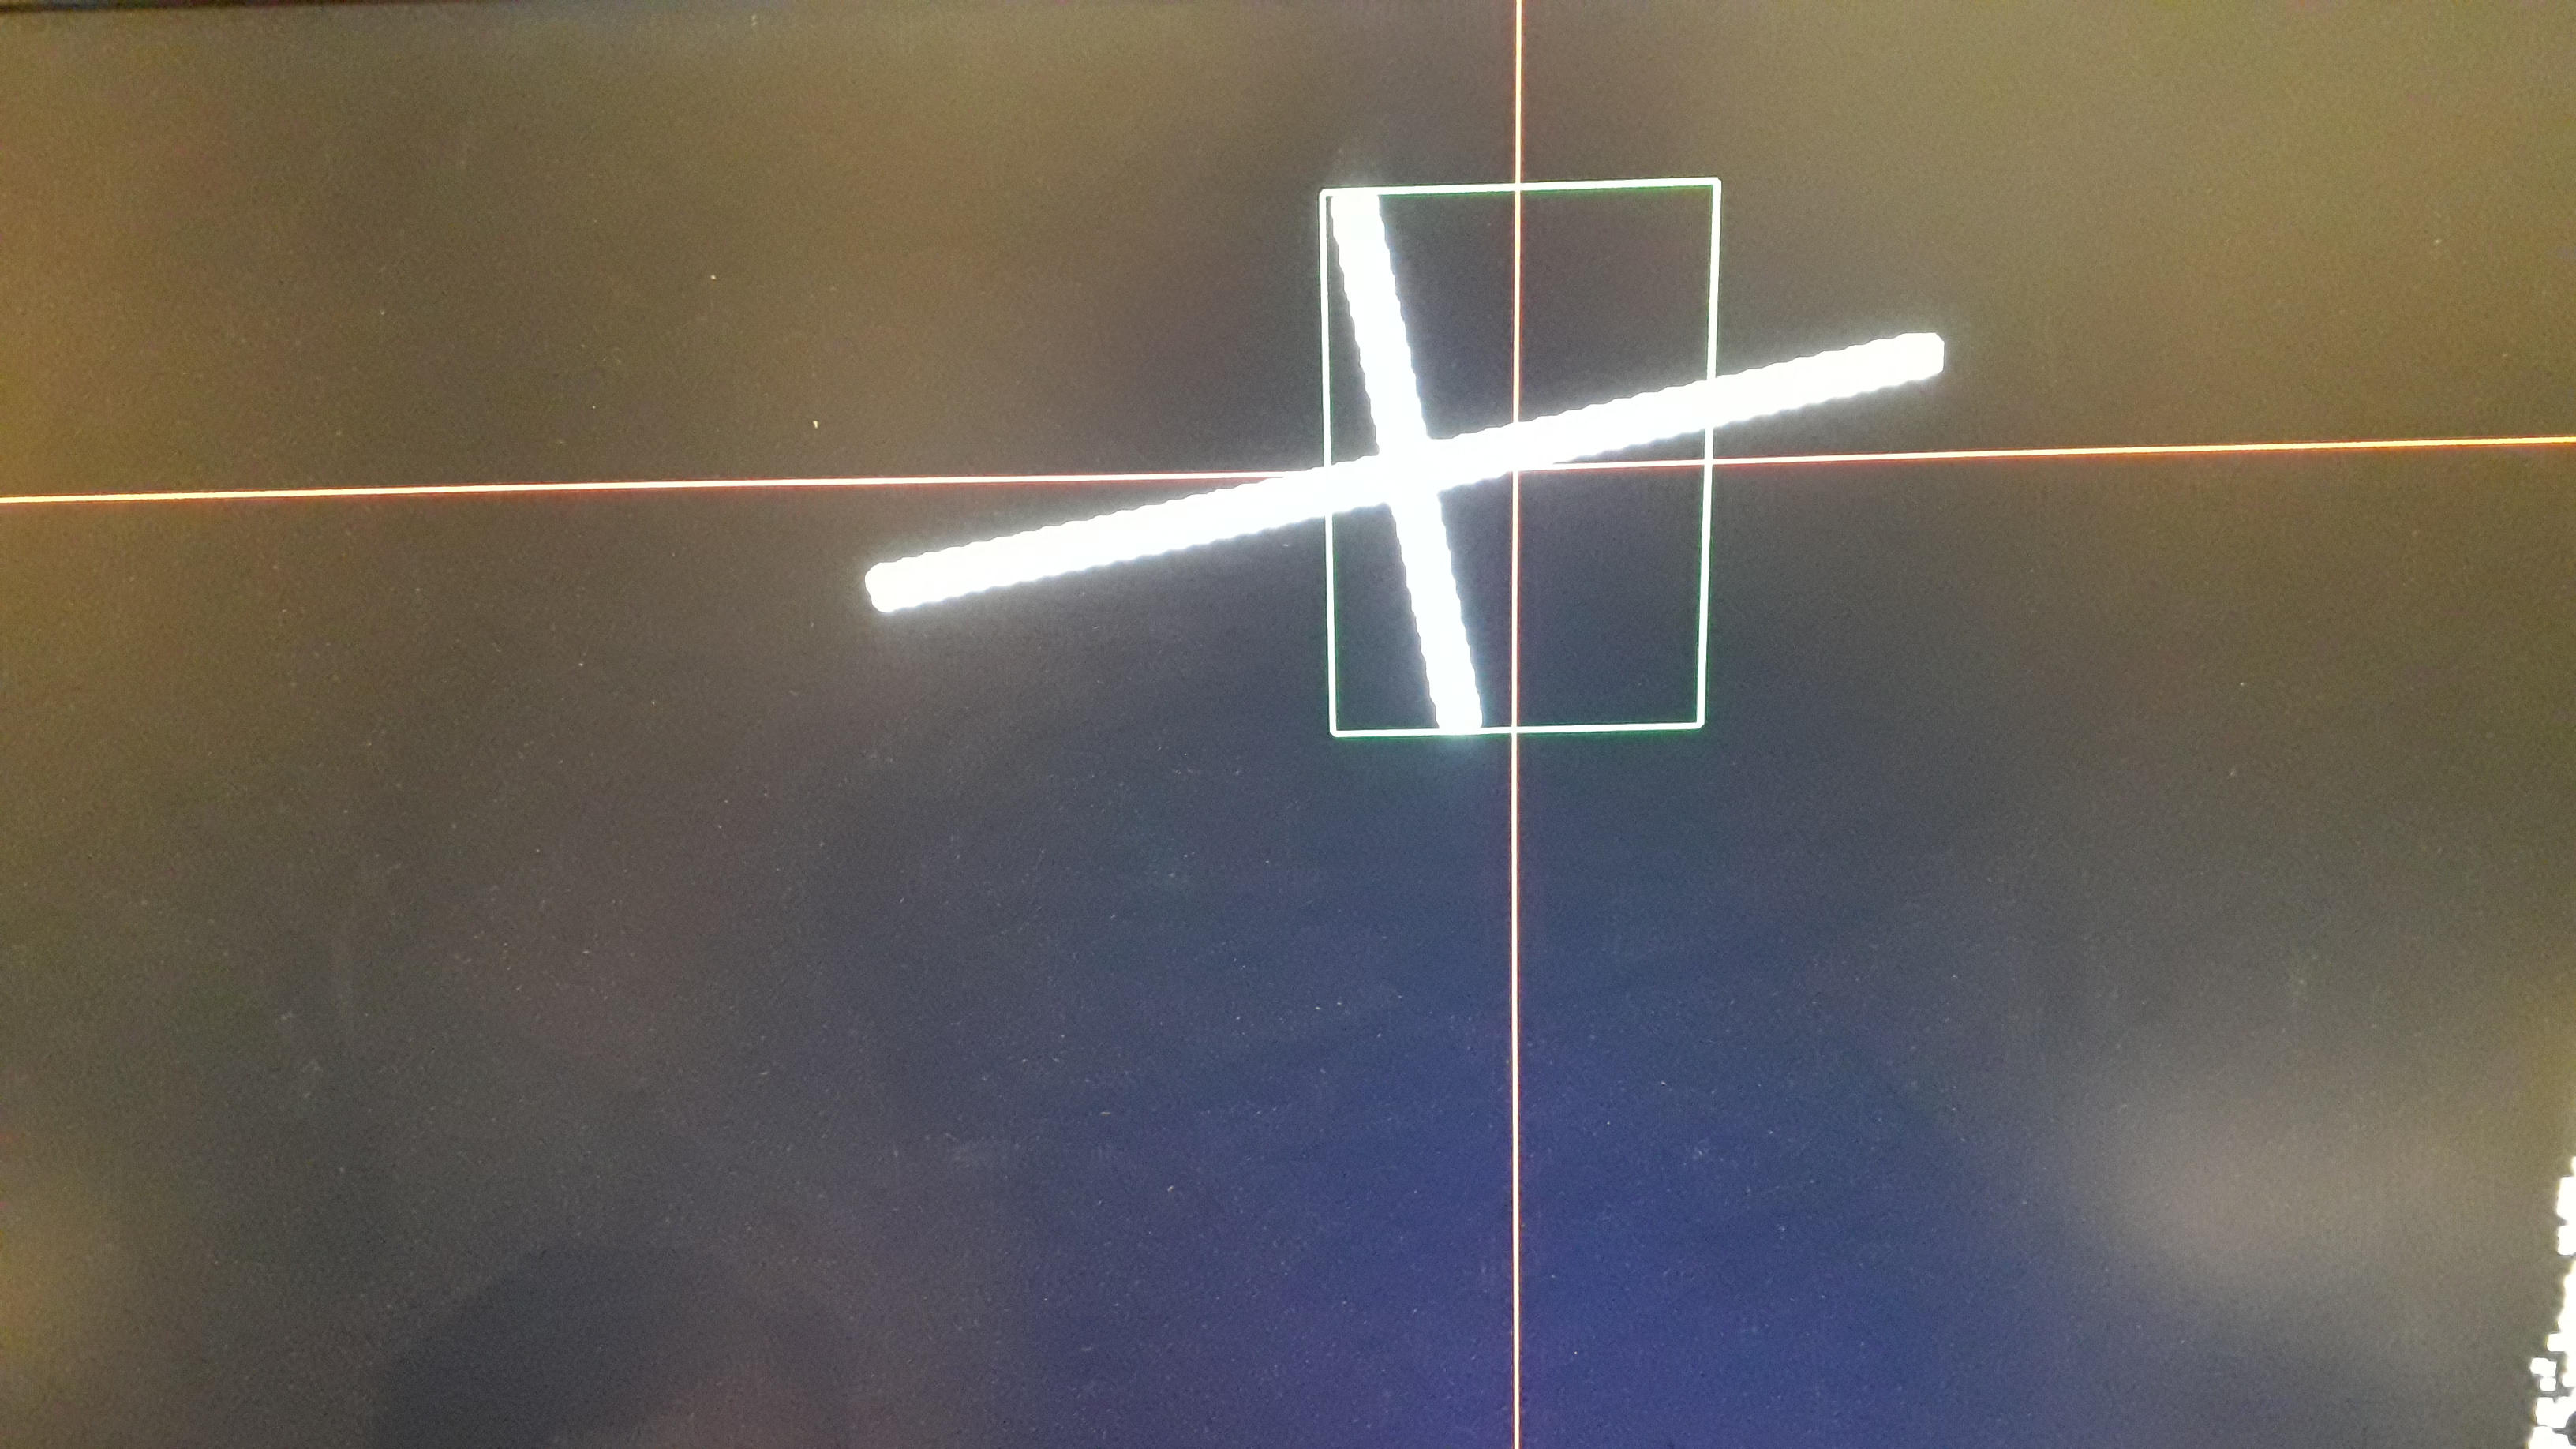
\includegraphics[width=\textwidth]{ind_niepoprawna.jpg}
		\caption{Obcięcie części znacznika ze~względu na brak etykiet}
		\label{fig:ind_niepoprawna}
	\end{subfigure}\\
	\caption{Rezultaty indeksacji w~zależności od~orientacji znacznika}
	\label{fig:rezultaty_ind}
\end{figure}
Aby możliwa była sprawna detekcja miejsca lądowania niezależnie od~orientacji markera, należało zmienić nieco koncepcję systemu. 
Innym podejściem było obliczanie środka ciężkości wszystkich białych pikseli. 
Eliminuje to~możliwość klasyfikacji obiektów ze~względu na~kształt (pozostaje klasyfikacja po~kolorze) i~tym samym czyni system podatnym na~zakłócenia. 
Pojawienie się w~kadrze innych grup pikseli o~tym samym kolorze spowoduje przesunięcie środka ciężkości.
Jednak w~warunkach testowych możliwe jest wypełnienie powierzchni kolorem silnie kontrastującym z~barwą znacznika. 
Z~tego powodu moduł wyznaczający środek ciężkości (podrozdział \ref{subsec:srodek_ciezosci}) był wykorzystywany podczas testowania rozwiązania.
Wyznaczanie pola figury i~prostokąta otaczającego (podrozdział \ref{subsec:prostokat_otaczajacy}) umożliwiało odrzucanie pewnych detekcji i~wysyłanie sygnału o~braku znalezienia znacznika. 
%TODO2 do tego akapitu powyżej proszę dopisać zdanie polu i prostokącie otaczającym oraz odwołać się do tych podrozdziałów poniżej. (wykonane)

\subsection{Wyznaczanie środka ciężkości}
\label{subsec:srodek_ciezosci}

Do wyznaczania środka ciężkości pikseli należących do~obiektu wykorzystano wzory \eqref{eq:m00}, \eqref{eq:m10} i~\eqref{eq:m01}.

\begin{equation}
\label{eq:m00}
m_{00}=\sum_{i=0}^{N-1}\sum_{j=0}^{M-1} x_{ij}
\end{equation}
\begin{equation}
\label{eq:m10}
m_{10}=\sum_{i=0}^{N-1}\sum_{j=0}^{M-1} i*x_{ij}
\end{equation}
\begin{equation}
\label{eq:m01}
m_{01}=\sum_{i=0}^{N-1}\sum_{j=0}^{M-1} j*x_{ij}
\end{equation}
gdzie:
\begin{eqwhere}[2cm]
	\item[$N$] szerokość obrazu w pikselach,
	\item[$M$] wysokość obrazu w pikselach,
	\item[$x_{ij}$] wartość piksela o~współrzędnych $i$, $j$ obrazu zbinaryzowanego.
\end{eqwhere}
Na ich podstawie obliczono środek ciężkości przy zastosowaniu wzorów \eqref{eq:xsc} i~\eqref{eq:ysc}.
\begin{equation}
\label{eq:xsc}
X_{sc}=\frac{m_{10}}{m_{00}}
\end{equation}
\begin{equation}
\label{eq:ysc}
Y_{sc}=\frac{m_{01}}{m_{00}}
\end{equation}
gdzie:
\begin{eqwhere}[2cm]
	\item[$X_{sc}$] współrzędna pozioma środka ciężkości,
	\item[$Y_{sc}$] współrzędna pionowa środka ciężkości.
\end{eqwhere}

W~module na podstawie sygnałów synchronizacji oraz wymiarów obrazka wyznaczono współrzędne aktualnie przetwarzanego piksela. 
Jeśli jest to piksel należący do obiektu, następuje zwiększenie wartości odpowiednich rejestrów zgodnie ze wzorami
\ref{eq:m00}, \ref{eq:m10} i~\ref{eq:m01}. 
Po przejściu przez całą ramkę obrazu wykonywane jest dzielenie na podstawie wzorów \ref{eq:xsc} i~\ref{eq:ysc}.

\subsection{Wyznaczanie prostokąta otaczającego i~pola powierzchni}
\label{subsec:prostokat_otaczajacy}

Znalezienie prostokąta otaczającego sprowadza się do wyznaczenia skrajnych jego punktów na górze, dole, po lewej oraz prawej stronie. 
Na podstawie sygnałów synchronizacji oraz wymiarów obrazka wyznaczano współrzędne aktualnie przetwarzanego piksela. 
Jeśli jest to piksel należący do obiektu, następuje inkrementacja jego pola powierzchni. 
Do~odpowiednich rejestrów trafiają wówczas również wartości współrzędnych piksela, jeśli wykraczają poza aktualną zawartość rejestrów:
\begin{itemize}
	\item do~rejestru zawierającego górny bok prostokąta trafi współrzędna wierszowa, jeśli będzie ona mniejsza od aktualnej,
	\item do~rejestru zawierającego dolny bok prostokąta trafi współrzędna wierszowa, jeśli będzie ona większa od aktualnej,
	\item do~rejestru zawierającego lewy bok prostokąta trafi współrzędna kolumnowa, jeśli będzie ona mniejsza od aktualnej,
	\item do~rejestru zawierającego prawy bok prostokąta trafi współrzędna kolumnowa, jeśli będzie ona większa od aktualnej,
\end{itemize}  
%Obliczeń pola powierzchni i~współrzędnych prostokąta otaczającego nie~wykonywano w~oddzielnym module, lecz stanowiły one część modułu indeksacji.
%TODO 2 indekacji czy tej analizy bez indekacji... bo teraz jest zamieszanie. 


\section{Algorytm sterowania}
\label{sec:algorytm_sterowania}

Informacjami o~detekcji lądowiska, koniecznymi do~realizacji algorytmu sterowania, są:
\begin{itemize}
	\item uchyb regulacji w~obu osiach, rozumiany jako odległość środka obrazu od~środka wykrytego lądowiska (centrum prostokąta otaczającego lub środka ciężkości),
	\item wiadomość o~znalezieniu znacznika. %TODO2 niestosowanie indeksacji nie wyklucza analizy kształtu (za małe pole, czy proporporcjie i może tego sygnału nie być)
\end{itemize}
%TODO2 tu jakaś informacja o tym, jak ta informacja jest przesyłana z PL do PS(wykonane)
Informacje te przesyłano z~części rekonfigurowalnej do~systemu procesorowego przy wykorzystaniu rejestrów AXI.

Dodatkowo, w~celu analiza działania systemu, istnieje możliwość podglądu przetworzonego obrazu na~monitorze, podłączonym poprzez port HDMI. 
Możliwy jest podgląd kolejnych etapów przetwarzania -- wybór etapu następuje przez zmianę ustawień przełączników na~płytce.

Algorytm sterowania bazuje na~dyskretnym regulatorze PID, zrealizowanym w~systemie procesorowym układu.
Regulacji podlegają składowe $x$ i~$y$ wektora położenia drona względem znacznika określającego lądowisko. 
Jeśli znacznik zostanie utracony z~pola widzenia kamery na~czas 1~sekundy, dron przechodzi w~tryb unoszenia się nad ziemią.

\section{Integracja płytki z autopilotem}
\label{sec:integracja_plytka_autopilot}

W~układzie Zynq z~karty ZYBO~Z7-20 wykorzystano interfejs UART0. 
Wyprowadzono piny TX i~RX z~systemu procesorowego i~podłączono je do~portu Pmod~JB. 
Po~stronie sterownika Pixhawk użyto portu TELEM~2. 
Szybkość transmisji to~115200~bodów.

Wysyłanie komend opiera się na~wykorzystaniu gotowych funkcji dostępnych w~sieci \cite{github_mavlink}.
Przygotowują one daną wiadomość zgodnie z~wymaganiami protokołu MAVLink. 
Następnie wywoływane są funkcje wysyłające przygotowaną tablicę bajtów przez odpowiedni UART. 
W~projekcie wykorzystano stworzone przy wykonywaniu pracy \cite{mgr} funkcje opakowujące kolejne etapy przetwarzania komend.
\section{Ewaluacja}
\label{sec:ewaluacja_sprzetu}
%TODO 2 Wtępniak
Zaimplementowane rozwiązania należało przetestować. Eksperymentem pozwalającym sprawdzić działanie laserowego czujnika odległości, przetwarzania wizyjnego i~algorytmu sterującego był test opisany w~podrozdziale \ref{sec:test_sterowania}. Test ten wymagał również integracji urządzeń na~platformie. Podrozdział \ref{sec:test_autopilota} opisuje natomiast test komunikacji karty i~sterownika drona. 
\subsection{Test sterowania}
\label{sec:test_sterowania}

Test ten polegał na ,,ręcznym'' wykonywaniu komend pochodzących z systemu procesorowego -- dron był trzymany w~ręce. 
Zaplanowano 3 fazy lotu: wznoszenie na określoną wysokość, kierowanie drona w~stronę znacznika oraz lądowanie.
Przy takim rozwiązaniu niemożliwe było zadawanie prędkości wynikającej z~regulacji PID. 
Ograniczono się do wysyłania komend: ,,w górę'', ,,w lewo'', ,,do przodu'' itp. 
Postarano się, aby podłoże miało kolor niebieski, kontrastujący z~czerwoną barwą znacznika. 
Zdjęcie z~eksperymentu przedstawiono na~Rys. \ref{fig:eksperyment}.\\
Test wykazał prawidłowe działanie laserowego czujnika odległości. 
Poprawnie podawane były również komendy dotyczące zmiany pozycji drona. 
\begin{figure}[h]
	\centering
	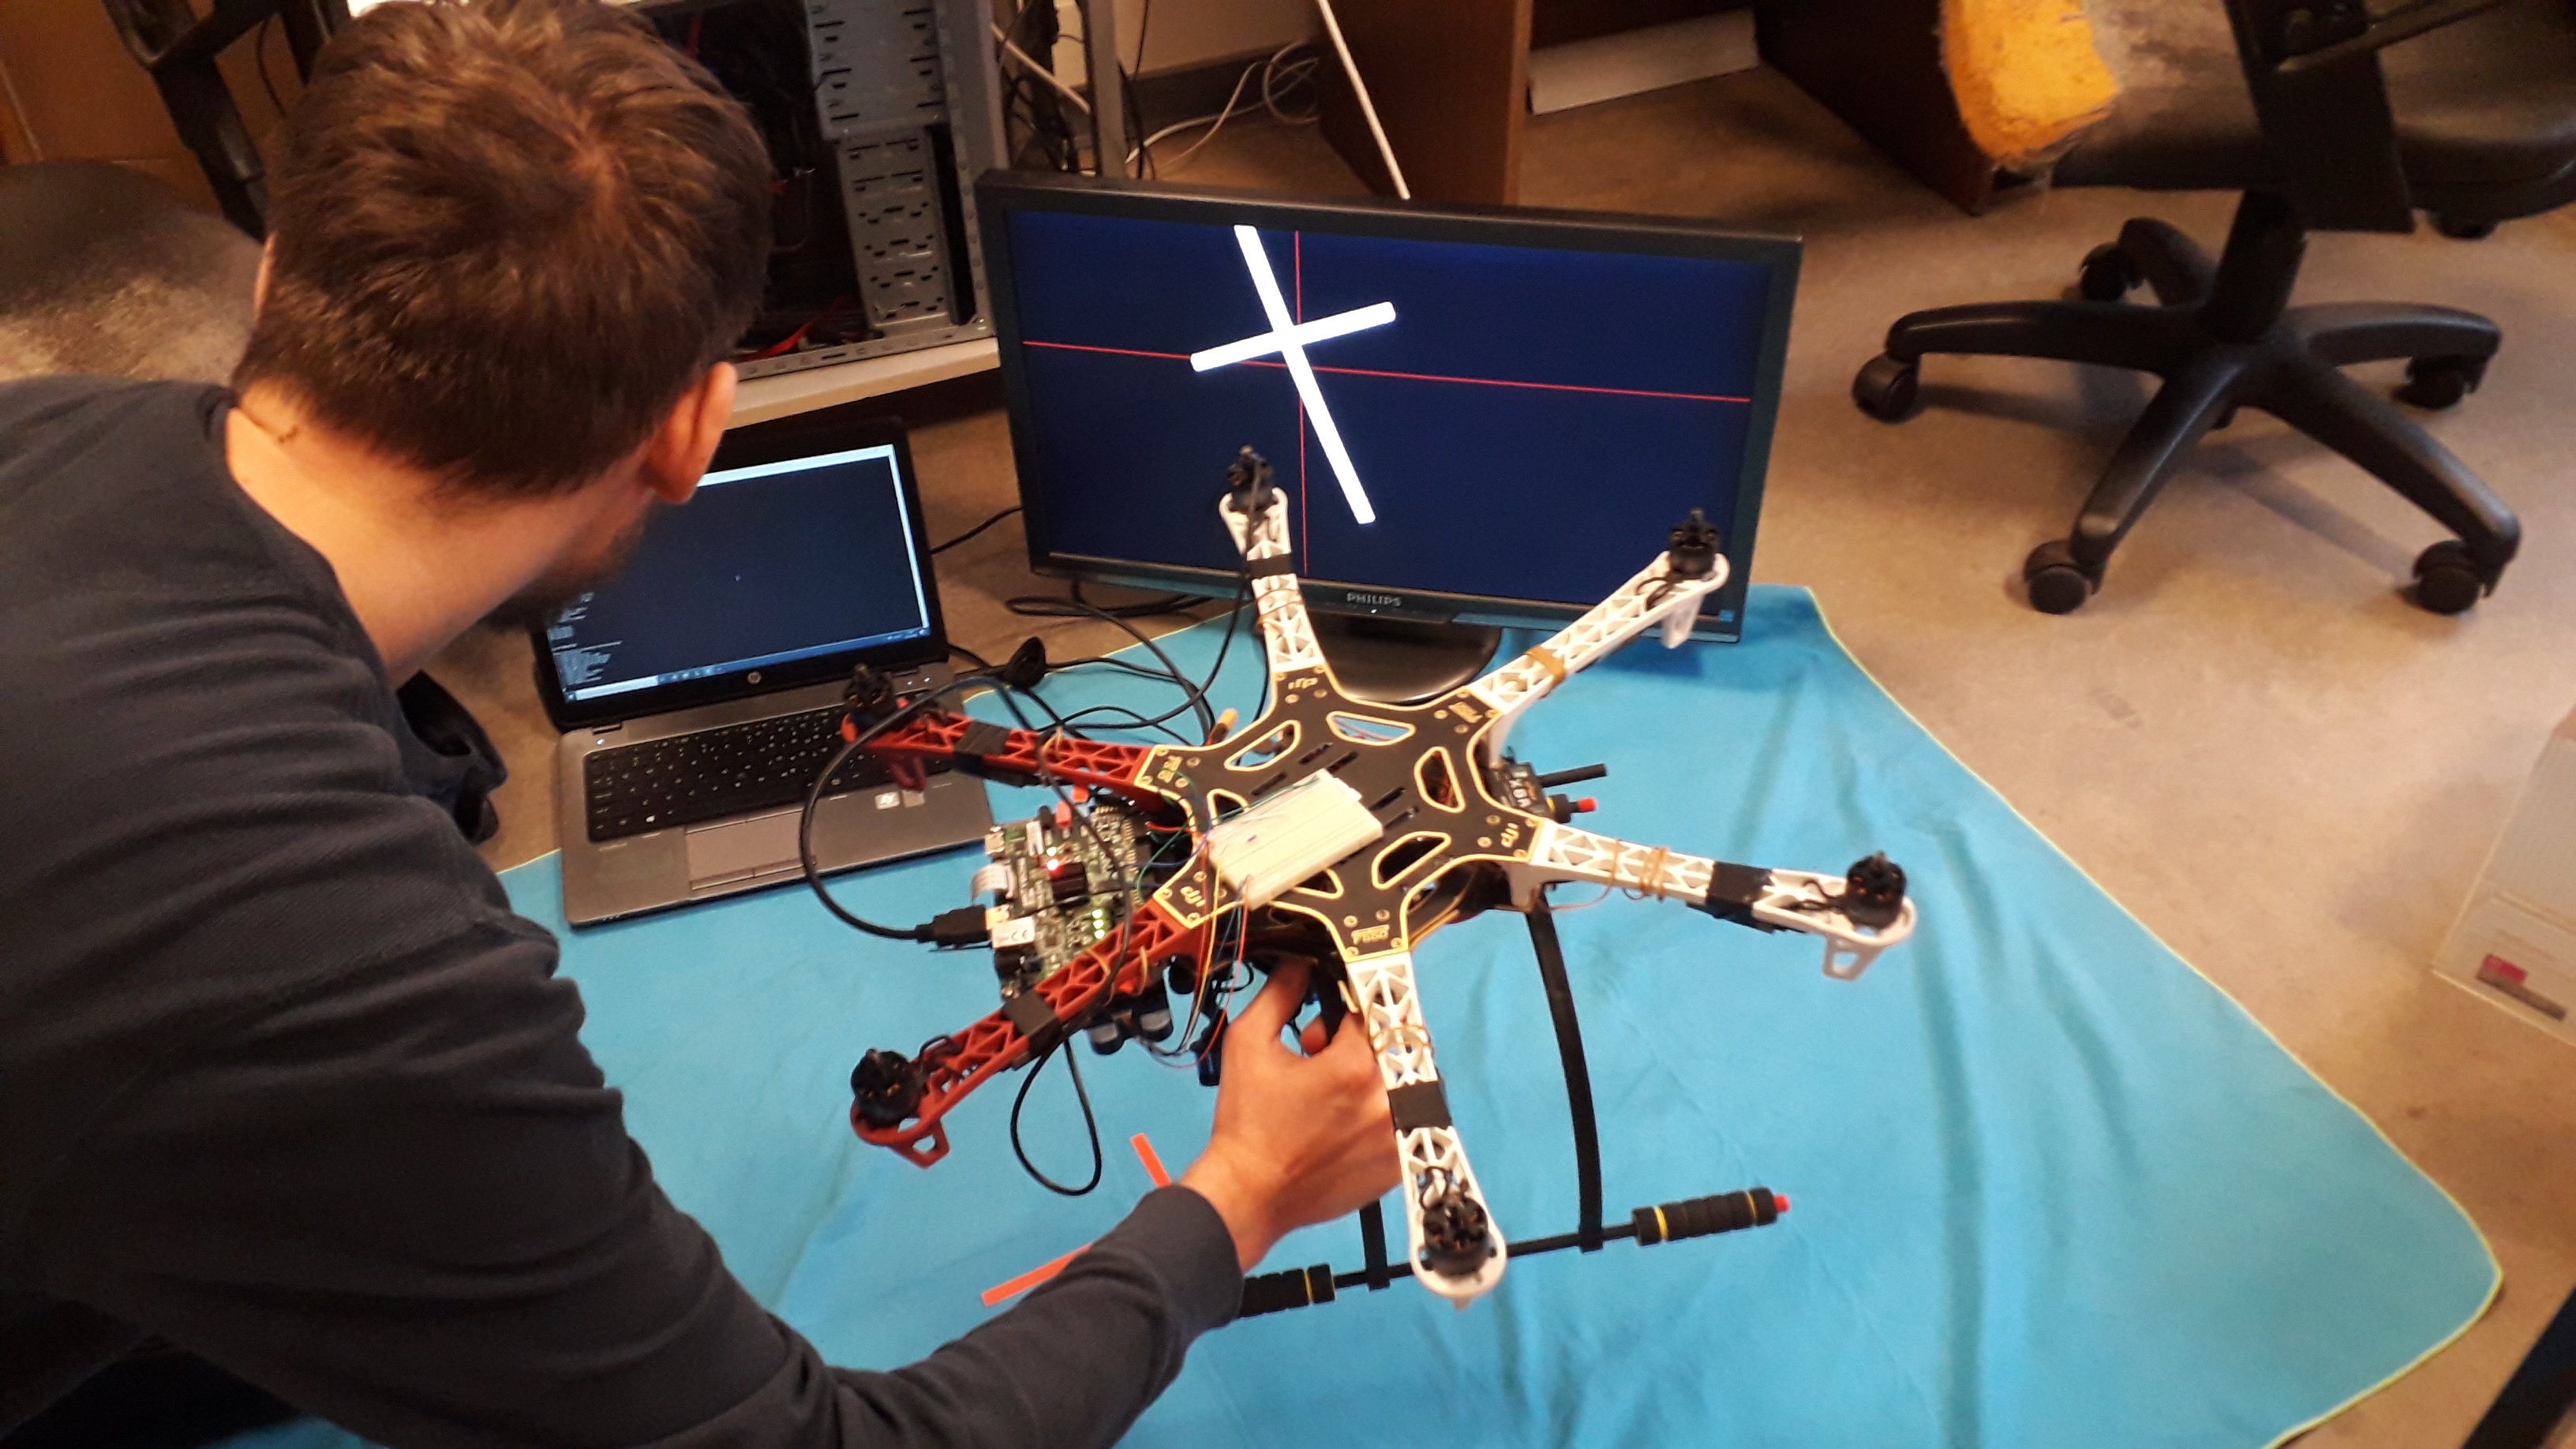
\includegraphics[width=\textwidth]{eksperyment.jpg}
	\caption{Zdjęcie z~eksperymentu. Kartę ZYBO~Z7-20 zamontowano z~przodu platformy. Poniżej umieszczono kamerę i~Lidar. Na~górze znajduje się płytka prototypowa do~łatwego łączenia komponentów.}
	\label{fig:eksperyment}
\end{figure}
\subsection{Test reakcji autopilota na zadawane komendy}
\label{sec:test_autopilota}
Test polegał na~wysyłaniu do~autopilota komend z~karty ZYBO~Z7-20. %TODO2 ZYBO to karta, układ to Zynq - proszę na to zwrócić uwagę.(wykonane)
Podczas eksperymentu śmigła drona były zdjęte. 
Wewnątrz budynku, możliwe było wysłanie komendy uzbrojenia silników w~trybie \textit{Stabilize}. 
Jak opisano w~rozdziale \ref{sec:autopilot}, nie jest to jednak tryb pozwalający na~wysyłanie komend ruchu.
Aby możliwe było kierowanie dronem, należało przeprowadzić eksperyment na~zewnątrz, w~celu utrzymania dostatecznie silnego sygnału GPS. 
Po~uaktywnieniu trybu \textit{Guided} wysłano kolejno komendy uzbrojenia silników, startu i~lotu z~określoną prędkością. 
Silniki reagowały na~wysyłane rozkazy.

Po~eksperymencie można było wysnuć wniosek o~poprawnej konfiguracji komunikacji pomiędzy kartą ZYBO, a~sterownikiem Pixhawk.

\section{Podsumowanie}
%TODO2 kilka słów o testach + jeszcze o komunikacji RF - nawet jak nie zadziałała
Test sterowania pokazał możliwość wykrycia lądowiska i~obliczania takiego sterowania dronem, aby lądowanie odbyło się w~wyznaczonym miejscu. Test komunikacji ze~sterownikiem pozwolił natomiast potwierdzić, że poprawnie utworzone zostało połączenie między platformą obliczeniową, a~autopilotem. 
\chapter{Podsumowanie}
\label{cha:Podsumowanie i kierunki dalszych prac}

W~pracy przedstawiono sprzętowo-programową realizację systemu wspomagającego autonomiczne lądowanie drona.
System zrealizowano w~układzie Zynq SoC na karcie ZYBO Z7-20. 
Część rekonfigurowalna pozwoliła na~szybkie przetwarzanie obrazu, natomiast system procesorowy umożliwił sprawną realizację algorytmu sterowania i~wysyłanie komend do~sterownika drona. 

Zaimplementowano dwie wersje systemu wizyjnego: z~indeksacją jednoprzebiegową i identyfikacją znacznika na podstawie koloru i~współczynnika kształtu oraz z~wyznaczaniem środka ciężkości i~identyfikacją markera przy użyciu jego barwy. 
Poprawną segmentację na~podstawie koloru przy niewielkiej zależności od~oświetlenia umożliwiła binaryzacja w~przestrzeni barw YCbCr, w~oparciu o~składowe Cb i~Cr. 
Zaprojektowano również taki znacznik, aby ułatwić jego wykrycie. 
Zaimplementowanie modułów mediany i~otwarcia pozwoliło na~filtrację obrazu.

Wprowadzenie do~układu sygnału z~czujnika lidar umożliwiło dokładną kontrolę wysokości.
%TODO radip
Zaimplementowano także regulację PID, której celem jest ustawienie drona nad znacznikiem. 
Eksperymenty pokazały możliwość wykonania symulowanego lotu testowego składającego się ze~startu, regulacji położenia i~lądowania w~wyznaczonym miejscu.
Przeprowadzone testy dowiodły również możliwości wysyłania do~sterowanika komend, między innymi dotyczących zmiany kierunku i~szybkości lotu. 

Kolejnym celem powinno być wykonanie lotu testowego (start -- regulacja położenia -- lądowanie) przy sterowaniu na~podstawie wizyjnego sprzężenia zwrotnego. 
Etapem pośrednim powinno być przeprowadzenie testu pozwalającego ustalić, jaką najmniejszą prędkość akceptuje autopilot, jaka największa prędkość powoduje ruch drona bez wyraźnego przechylenia i~pochylenia oraz z~jaką częstotliwością mogą być wysyłane komendy. 
Te~informacje pozwoliłyby na~dobór nastaw regulatora. 
W~przypadku niemożliwości realizacji komend z~odpowiednią częstotliwością rozważyć można inną koncepcję: na~podstawie wysokości i~aktualnej pozycji znacznika na~obrazie można byłoby wyznaczać od~razu przesunięcie (zamiast prędkości), które doprowadziłoby dron ponad znacznik. Zadawanie przesunięcia również jest wspierane przez oprogramowanie ArduPilot. Takie podejście wymagałoby przeprowadzenia testów odległości od~znacznika w~terenie, w~zależności od~tej odległości na~obrazie. %TODO2 Nie bardzo to rozumiem... (doprecyzowane)

Powyższe działania możliwe są~przy zastosowaniu komponentów użytych w~projekcie. 
Użycie kamery o~większym kącie widzenia pozwoliłoby jednak na~detekcję lądowiska z~większej odległości.
Innym kierunkiem dalszych pracach może być próba wykonania lądowania na~poruszającej się platformie. 
Analiza literatury naukowej dostarczyła informacji co~do~niezbędnych działań, jakie musi wykonywać taki system. 
Są~to: śledzenie lądowiska, predykcja ruchu lądowiska, generacja trajektorii pozwalających dotrzeć do~celu, wybór jednej z~dopuszczalnych oraz realizacja odpowiedniego sterowania.

%TODO + Dodatek A. Spis zawartości CD, która będzie dla mnie (nie dziekanatu).
\appendix
\chapter{Spis zawartości płyty CD}
Na dołączonej do~pracy płycie CD znajdują się następujące foldery:
\begin{itemize}
	\item Matlab -- zawiera pliki modeli programowych, testów, obróbki obrazów oraz zdjęcia niezbędne do ich uruchomienia,
	\item Vivado -- zawiera projekt główny oraz testowy, wykorzystywany do~komunikacji z~autopilotem,
	\item Tex -- zawiera pliki tekstowe \LaTeX wraz z~rysunkami pojawiającymi się w~tekście.
\end{itemize}
%---------------------------------------------------------------------------

%\chapter{Przykłady elementów pracy dyplomowej}

\section{Liczba}

Pakiet \texttt{siunitx} zadba o to, by liczba została poprawnie sformatowana: \\
\begin{center}
	\num{1234567890.0987654321}
\end{center}


\section{Rysunek}

Pakiet \texttt{subcaption} pozwala na umieszczanie w podpisie rysunku odnośników do ,,podilustracji'': \\

\begin{figure}[h]
	\centering
	\begin{subfigure}{0.35\textwidth}
		\centering
		\framebox[2.0\width]{A}
		\subcaption{\label{subfigure_a}}
	\end{subfigure}
	\begin{subfigure}{0.35\textwidth}
		\centering
		\framebox[2.0\width]{B}
		\subcaption{\label{subfigure_b}}
	\end{subfigure}
	
	\caption{\label{fig:subcaption_example}Przykład użycia \texttt{\textbackslash subcaption}: \protect\subref{subfigure_a} litera A, \protect\subref{subfigure_b} litera B.}
\end{figure}

\section{Tabela}

Pakiet \texttt{threeparttable} umożliwia dodanie do tabeli adnotacji: \\

\begin{table}[h]
	\centering
	
	\begin{threeparttable}
		\caption{Przykład tabeli}
		\label{tab:table_example}
		
		\begin{tabularx}{0.6\textwidth}{C{1}}
			\toprule
			\thead{Nagłówek\tnote{a}} \\
			\midrule
			Tekst 1 \\
			Tekst 2 \\
			\bottomrule
		\end{tabularx}
		
		\begin{tablenotes}
			\footnotesize
			\item[a] Jakiś komentarz\textellipsis
		\end{tablenotes}
		
	\end{threeparttable}
\end{table}

\section{Wzory matematyczne}

Czasem zachodzi potrzeba wytłumaczenia znaczenia symboli użytych w równaniu. Można to zrobić z użyciem zdefiniowanego na potrzeby niniejszej klasy środowiska \texttt{eqwhere}.

\begin{equation}
E = mc^2
\end{equation}
gdzie
\begin{eqwhere}[2cm]
	\item[$m$] masa
	\item[$c$] prędkość światła w próżni
\end{eqwhere}

Odległość półpauzy od lewego marginesu należy dobrać pod kątem najdłuższego symbolu (bądź listy symboli) poprzez odpowiednie ustawienie parametru tego środowiska (domyślnie: 2 cm).

%\chapter{Wprowadzenie}
\label{cha:wprowadzenie}

\LaTeX~jest systemem składu umożliwiającym tworzenie dowolnego typu dokumentów (w~szczególności naukowych i technicznych) o wysokiej jakości typograficznej (\cite{Dil00}, \cite{Lam92}). Wysoka jakość składu jest niezależna od rozmiaru dokumentu -- zaczynając od krótkich listów do bardzo grubych książek. \LaTeX~automatyzuje wiele prac związanych ze składaniem dokumentów np.: referencje, cytowania, generowanie spisów (treśli, rysunków, symboli itp.) itd.

\LaTeX~jest zestawem instrukcji umożliwiających autorom skład i wydruk ich prac na najwyższym poziomie typograficznym. Do formatowania dokumentu \LaTeX~stosuje \TeX a (wymiawamy 'tech' -- greckie litery $\tau$, $\epsilon$, $\chi$). Korzystając z~systemu składu \LaTeX~mamy za zadanie przygotować jedynie tekst źródłowy, cały ciężar składania, formatowania dokumentu przejmuje na siebie system.

%---------------------------------------------------------------------------

\section{Cele pracy}
\label{sec:celePracy}


Celem poniższej pracy jest zapoznanie studentów z systemem \LaTeX~w zakresie umożliwiającym im samodzielne, profesjonalne złożenie pracy dyplomowej w systemie \LaTeX.

\subsection{Jakiś tytuł}
Przykład
\subsubsection{Jakiś tytuł w subsubsection}


\subsection{Jakiś tytuł 2}

%---------------------------------------------------------------------------

\section{Zawartość pracy}
\label{sec:zawartoscPracy}

W rodziale~\ref{cha:pierwszyDokument} przedstawiono podstawowe informacje dotyczące struktury dokumentów w \LaTeX u. Alvis~\cite{Alvis2011} jest językiem 



















%\chapter{Pierwszy dokument}
\label{cha:pierwszyDokument}

W rozdziale tym przedstawiono podstawowe informacje dotyczące struktury prostych plików \LaTeX a. Omówiono również metody kompilacji plików z zastosowaniem programów \emph{latex} oraz \emph{pdflatex}.

%---------------------------------------------------------------------------

\section{Struktura dokumentu}
\label{sec:strukturaDokumentu}

Plik \LaTeX owy jest plikiem tekstowym, który oprócz tekstu zawiera polecenia formatujące ten tekst (analogicznie do języka HTML). Plik składa się z dwóch części:
\begin{enumerate}%[1)]
\item Preambuły -- określającej klasę dokumentu oraz zawierającej m.in. polecenia dołączającej dodatkowe pakiety;

\item Części głównej -- zawierającej zasadniczą treść dokumentu.
\end{enumerate}


\begin{lstlisting}
\documentclass[a4paper,12pt]{article}      % preambuła
\usepackage[polish]{babel}
\usepackage[utf8]{inputenc}
\usepackage[T1]{fontenc}
\usepackage{times}

\begin{document}                           % część główna

\section{Sztuczne życie}

% treść
% ąśężźćńłóĘŚĄŻŹĆŃÓŁ

\end{document}
\end{lstlisting}

Nie ma żadnych przeciwskazań do tworzenia dokumentów w~\LaTeX u w~języku polskim. Plik źródłowy jest zwykłym plikiem tekstowym i~do jego przygotowania można użyć dowolnego edytora tekstów, a~polskie znaki wprowadzać używając prawego klawisza \texttt{Alt}. Jeżeli po kompilacji dokumentu polskie znaki nie są wyświetlane poprawnie, to na 95\% źle określono sposób kodowania znaków (należy zmienić opcje wykorzystywanych pakietów).


%---------------------------------------------------------------------------

\section{Kompilacja}
\label{sec:kompilacja}


Załóżmy, że przygotowany przez nas dokument zapisany jest w pliku \texttt{test.tex}. Kolejno wykonane poniższe polecenia (pod warunkiem, że w pierwszym przypadku nie wykryto błędów i kompilacja zakończyła się sukcesem) pozwalają uzyskać nasz dokument w formacie pdf:
\begin{lstlisting}
latex test.tex
dvips test.dvi -o test.ps
ps2pdf test.ps
\end{lstlisting}
%
lub za pomocą PDF\LaTeX:
\begin{lstlisting}
pdflatex test.tex
\end{lstlisting}

Przy pierwszej kompilacji po zmiane tekstu, dodaniu nowych etykiet itp., \LaTeX~tworzy sobie spis rozdziałów, obrazków, tabel itp., a dopiero przy następnej kompilacji korzysta z tych informacji.

W pierwszym przypadku rysunki powinny być przygotowane w~formacie eps, a~w~drugim w~formacie pdf. Ponadto, jeżeli używamy polecenia \texttt{pdflatex test.tex} można wstawiać grafikę bitową (np. w formacie jpg).



%---------------------------------------------------------------------------

\section{Narzędzia}
\label{sec:narzedzia}


Do przygotowania pliku źródłowego może zostać wykorzystany dowolny edytor tekstowy. Niektóre edytory, np. GEdit, mają wbudowane moduły ułatwiające składanie tekstów w LaTeXu (kolorowanie składni, skrypty kompilacji, itp.).

Jednym z bardziej znanych środowisk do składania dokumentów  \LaTeX a jest {\em TeXstudio}, oferujące kompletne środowisko pracy. Zobacz: \url{http://www.texstudio.org}


Bardzo dobrym środowiskiem jest również edytor gEdit z wtyczką obsługującą \LaTeX a. Jest to standardowy edytor środowiska Gnome. Po instalacji wtyczki obsługującej \LaTeX~ zamienia się w wygodne i szybkie środowisko pracy.

\textbf{Dla testu łamania stron powtórzenia powyższego tekstu.}


Do przygotowania pliku źródłowego może zostać wykorzystany dowolny edytor tekstowy. Niektóre edytory, np. GEdit, mają wbudowane moduły ułatwiające składanie tekstów w LaTeXu (kolorowanie składni, skrypty kompilacji, itp.).
Jednym z bardziej znanych środowisk do składania dokumentów  \LaTeX a jest {\em TeXstudio}, oferujące kompletne środowisko pracy. Zobacz: \url{http://www.texstudio.org}
Bardzo dobrym środowiskiem jest również edytor gEdit z wtyczką obsługującą \LaTeX a. Jest to standardowy edytor środowiska Gnome. Po instalacji wtyczki obsługującej \LaTeX~ zamienia się w wygodne i szybkie środowisko pracy.
Po instalacji wtyczki obsługującej \LaTeX~ zamienia się w wygodne i szybkie środowisko pracy.

Do przygotowania pliku źródłowego może zostać wykorzystany dowolny edytor tekstowy. Niektóre edytory, np. GEdit, mają wbudowane moduły ułatwiające składanie tekstów w LaTeXu (kolorowanie składni, skrypty kompilacji, itp. itd. itp.).
Jednym z bardziej znanych środowisk do składania dokumentów  \LaTeX a jest {\em TeXstudio}, oferujące kompletne środowisko pracy. Zobacz: \url{http://www.texstudio.org}
Bardzo dobrym środowiskiem jest również edytor gEdit z wtyczką obsługującą \LaTeX a. Jest to standardowy edytor środowiska Gnome. Po instalacji wtyczki obsługującej \LaTeX~ zamienia się w wygodne i szybkie środowisko pracy.

Do przygotowania pliku źródłowego może zostać wykorzystany dowolny edytor tekstowy. Niektóre edytory, np. GEdit, mają wbudowane moduły ułatwiające składanie tekstów w LaTeXu (kolorowanie składni, skrypty kompilacji, itp.).
Jednym z bardziej znanych środowisk do składania dokumentów  \LaTeX a jest {\em TeXstudio}, oferujące kompletne środowisko pracy. Zobacz: \url{http://www.texstudio.org}
Bardzo dobrym środowiskiem jest również edytor gEdit z wtyczką obsługującą \LaTeX a. Jest to standardowy edytor środowiska Gnome. Po instalacji wtyczki obsługującej \LaTeX~ zamienia się w wygodne i szybkie środowisko pracy.

%---------------------------------------------------------------------------

\section{Przygotowanie dokumentu}
\label{sec:przygotowanieDokumentu}

Plik źródłowy \LaTeX a jest zwykłym plikiem tekstowym. Przygotowując plik
źródłowy warto wiedzieć o kilku szczegółach:

\begin{itemize}
\item
Poszczególne słowa oddzielamy spacjami, przy czym ilość spacji nie ma znaczenia.
Po kompilacji wielokrotne spacje i tak będą wyglądały jak pojedyncza spacja.
Aby uzyskać {\em twardą spację}, zamiast znaku spacji należy użyć znaku {\em
tyldy}.

\item
Znakiem końca akapitu jest pusta linia (ilość pusty linii nie ma znaczenia), a
nie znaki przejścia do nowej linii.

\item
\LaTeX~sam formatuje tekst. \textbf{Nie starajmy się go poprawiać}, chyba, że
naprawdę wiemy co robimy.
\end{itemize} 



%\chapter{Rozdział 4}
\label{cha:wprowadzenie}

\LaTeX~jest systemem składu umożliwiającym tworzenie dowolnego typu dokumentów (w~szczególności naukowych i technicznych) o wysokiej jakości typograficznej (\cite{Dil00}, \cite{Lam92}). Wysoka jakość składu jest niezależna od rozmiaru dokumentu -- zaczynając od krótkich listów do bardzo grubych książek. \LaTeX~automatyzuje wiele prac związanych ze składaniem dokumentów np.: referencje, cytowania, generowanie spisów (treśli, rysunków, symboli itp.) itd.

\LaTeX~jest zestawem instrukcji umożliwiających autorom skład i wydruk ich prac na najwyższym poziomie typograficznym. Do formatowania dokumentu \LaTeX~stosuje \TeX a (wymiawamy 'tech' -- greckie litery $\tau$, $\epsilon$, $\chi$). Korzystając z~systemu składu \LaTeX~mamy za zadanie przygotować jedynie tekst źródłowy, cały ciężar składania, formatowania dokumentu przejmuje na siebie system.

%---------------------------------------------------------------------------

\section{Cele pracy}
\label{sec:celePracy}


Celem poniższej pracy jest zapoznanie studentów z systemem \LaTeX~w zakresie umożliwiającym im samodzielne, profesjonalne złożenie pracy dyplomowej w systemie \LaTeX.

\subsection{Jakiś tytuł}
Przykład
\subsubsection{Jakiś tytuł w subsubsection}


\subsection{Jakiś tytuł 2}

%---------------------------------------------------------------------------

\section{Zawartość pracy}
\label{sec:zawartoscPracy}

W rodziale~\ref{cha:pierwszyDokument} przedstawiono podstawowe informacje dotyczące struktury dokumentów w \LaTeX u. Alvis~\cite{Alvis2011} jest językiem 

%\chapter{Testy}

\section{Test URL-a}

Wejdź na stronę \url{https://www.google.pl/} i wpisz szukane zdanie.

\clearpage

\section{Test dzielenia wdów}

Lorem ipsum dolor sit amet, ex est alia dolorem commune. Duo modo errem no. Ea harum doming atomorum mei. Consul animal malorum cu qui, sumo dicta graece an est, vim ei clita regione.

Vel eu quando doming fastidii, mei graeco indoctum an, legere theophrastus in pro. Te mei probatus eleifend interpretaris. Est no autem liber vituperatoribus, cu mea dicam constituto. Ea laudem tritani consectetuer sit, sanctus patrioque expetendis vix in. Duo id fugit adversarium signiferumque, an quot modus molestiae qui.

Ut paulo definiebas pro. Mea an quod esse. Et atomorum facilisis moderatius sit. Graeco iudicabit forensibus in vel. Eam cu lorem aeterno offendit, cu vix nulla congue posidonium. Vel lucilius evertitur vituperata no.

Mea eu graecis prodesset. Et tota eius nec. Ei etiam oratio has, vel ei homero eripuit invenire. Sed ex errem intellegebat, sea et elitr intellegat constituto. Nostro voluptua accusamus eos in, ei sale admodum has. Vim ne consetetur reformidans, ad has malis recusabo persequeris, per etiam virtute invenire in.

Te nihil eruditi eam, sit aperiam accusam mediocritatem at. Nec ne nonumy dictas disputationi, vis ridens sadipscing ex. Harum euripidis ex vix, at consetetur instructior signiferumque mel, at mei elitr honestatis. Id sit congue vituperata. Temporibus eloquentiam no eum.

Pro id esse phaedrum, nostro iudicabit eos ut. Sit ea aperiam alienum, harum audiam voluptua cu usu. Iudico invenire te vel, id suscipit disputando pri. Ut sumo expetenda mea.

Cum at idque nullam aperiam, vis ex aeque ponderum luptatum. Vix soluta graeco dissentiet ut, ut est reque periculis similique, ut dicta dicant repudiare sea. Ne dolor legendos signiferumque ius, at eirmod convenire qui. Suas numquam conceptam mei ex. Autem homero eos et, sea dicta alienum iudicabit ut.

Ea duo consulatu vulputate, id elit perpetua cum. His ei aeque saepe audiam. Prompta laoreet facilisi ne sed, per hinc consetetur te, oratio fuisset ullamcorper mel at. Quis suscipiantur ne nec, agam efficiendi usu in.

Vis eu iuvaret singulis appellantur, usu ex saepe omittantur. Sed possit mnesarchum at, usu illum choro oratio in, et debet dolor vix. Mel aperiri suscipiantur ne, te per illum fuisset, lorem pericula mei ad. Pri id tale lucilius dissentiet, id sea sonet expetenda. Agam sensibus persequeris sed no, eum at tamquam sanctus.

Omnis exerci soleat ut vis. Rebum vidisse sea ex. Ius animal gubergren efficiantur ad, mollis probatus nec ut. Meis platonem ex vel, ut qui tale tritani equidem. Vide meis fuisset mel at, nam an assum delenit gubergren. No illum reprimique vim, te augue nullam per, ludus dicant suscipiantur ne sed.

An pri mediocrem deseruisse, ad sumo audire dissentiet sit. Sit ea civibus lobortis. Etiam ceteros commune ei vis. Pro ei equidem vivendo. Quo ne prima periculis omittantur, ex rebum veritus sit, ei dolor maiestatis mea.

\subsection{Lorem ipsum}

Et mel munere quodsi sapientem. Essent legimus ne pro. Est ornatus definiebas et. No habemus docendi ius, purto sapientem mei at. Tamquam vivendo necessitatibus has at, no habemus praesent nec. No quo modus iudicabit scriptorem. Modus intellegebat ea vim. Cu ius lorem regione offendit, ne accusata sensibus vituperatoribus quo. Sit ut iuvaret indoctum. Ut mea sale justo. Sapientem definitionem ius eu, at sea quem doming. Facete conclusionemque ut nec, vix at duis eius. Eos quot consequuntur et, ornatus liberavisse ne mei.

Per an dicam commodo tractatos, usu in timeam numquam tacimates. Case delectus eu sea, usu audiam eleifend tincidunt id, nec at decore discere mentitum. Ut elit veri eloquentiam his, ceteros tractatos ea has. Duo impetus scribentur et, eu quo errem everti, ad recusabo consulatu ius. Fastidii comprehensam pri ea, ex duo augue quando denique. Eos aeterno deserunt sententiae cu, ius quas tation patrioque ex.

Id autem scripta explicari nec, congue quidam possit te sit. Et usu ipsum bonorum graecis, ferri verear deterruisset eum cu. Purto porro accommodare cu vim. Cum ei tritani pertinacia voluptaria.



% itd.
% \appendix
% \include{dodatekA}
% \include{dodatekB}
% itd.

\printbibliography

%TODO + Dodatek A. Spis zawartości CD, która będzie dla mnie (nie dziekanatu).
\appendix
\chapter{Spis zawartości płyty CD}
Na dołączonej do~pracy płycie CD znajdują się następujące foldery:
\begin{itemize}
	\item Matlab -- zawiera pliki modeli programowych, testów, obróbki obrazów oraz zdjęcia niezbędne do ich uruchomienia,
	\item Vivado -- zawiera projekt główny oraz testowy, wykorzystywany do~komunikacji z~autopilotem,
	\item Tex -- zawiera pliki tekstowe \LaTeX wraz z~rysunkami pojawiającymi się w~tekście.
\end{itemize}

\end{document}
